% main.tex
\documentclass[12pt]{article}

% Load the preamble from the separate file
% Options for packages loaded elsewhere
\usepackage{xcolor}
% In your preamble, open an output file:

\PassOptionsToPackage{unicode}{hyperref}
\PassOptionsToPackage{hyphens}{url}

% Basic packages
\usepackage{amsmath,amssymb}

% Remove section numbering
\setcounter{secnumdepth}{-\maxdimen}

% Font setup depending on engine
\usepackage{iftex}
\ifPDFTeX
  \usepackage[T1]{fontenc}
  \usepackage{textcomp} % provides euro and other symbols
\else % for LuaTeX or XeTeX
  \usepackage{unicode-math} % also loads fontspec
  \defaultfontfeatures{Scale=MatchLowercase}
  \defaultfontfeatures[\rmfamily]{Ligatures=TeX,Scale=1}
\fi

\usepackage{lmodern}

\usepackage[utf8]{inputenc}
\DeclareUnicodeCharacter{03B2}{\ensuremath{\beta}}
\DeclareUnicodeCharacter{1D6FD}{\ensuremath{\beta}}
\DeclareUnicodeCharacter{2248}{\ensuremath{\approx}}
\DeclareUnicodeCharacter{0394}{\ensuremath{\Delta}}
\DeclareUnicodeCharacter{0470}{\ensuremath{\Psi}}

% Use upquote if available (for straight quotes in verbatim)
\IfFileExists{upquote.sty}{\usepackage{upquote}}{}

% Use microtype if available
\IfFileExists{microtype.sty}{%
  \usepackage{microtype}%
  \UseMicrotypeSet[protrusion]{basicmath} % disable protrusion for tt fonts
}{}

% Adjust paragraph spacing for non-KOMA classes
\makeatletter
\@ifundefined{KOMAClassName}{%
  \IfFileExists{parskip.sty}{%
    \usepackage{parskip}%
  }{%
    \setlength{\parindent}{0pt}%
    \setlength{\parskip}{6pt plus 2pt minus 1pt}%
  }%
}{%
  \KOMAoptions{parskip=half}%
}
\makeatother

\usepackage{graphicx}

% Define a macro for scaling images to fit within the text area
\makeatletter
\newsavebox\pandoc@box
\newcommand*\pandocbounded[1]{%
  \sbox\pandoc@box{#1}%
  \Gscale@div\@tempa{\textheight}{\dimexpr\ht\pandoc@box+\dp\pandoc@box\relax}%
  \Gscale@div\@tempb{\linewidth}{\wd\pandoc@box}%
  \ifdim\@tempb\p@<\@tempa\p@\let\@tempa\@tempb\fi
  \ifdim\@tempa\p@<\p@\scalebox{\@tempa}{\usebox\pandoc@box}%
  \else\usebox{\pandoc@box}%
  \fi
}
\makeatother

% Set default figure placement to htbp
\def\fps@figure{htbp}

% Load color and highlighting packages for LuaTeX vs. others
% \ifLuaTeX
%   \usepackage{luacolor}
%   \usepackage[soul]{lua-ul}
% \else
%   \usepackage{soul}
% \fi

% Prevent overfull lines
\setlength{\emergencystretch}{3em}

% Define tight list formatting (from pandoc)
\providecommand{\tightlist}{%
  \setlength{\itemsep}{0pt}%
  \setlength{\parskip}{0pt}%
}

% Hyperlinks and bookmarks
\usepackage{bookmark}
\IfFileExists{xurl.sty}{\usepackage{xurl}}{} % allow URL line breaks
\urlstyle{same}
\hypersetup{
  hidelinks,
  pdfcreator={LaTeX via pandoc}
}

% Page geometry and additional formatting
\usepackage[margin=1in]{geometry}
\usepackage{lineno}   % for line numbering
\usepackage{setspace}

\usepackage[backend=biber, sorting=none,style=numeric-comp]{biblatex} % you can choose a different style if you like
%\usepackage[backend=biber]{biblatex} 
\addbibresource{references.bib} 

\usepackage{booktabs}  % For nicer horizontal lines
\usepackage{graphicx}

\usepackage{hyperref} % For clickable references and \phantomsection

% New counter for supplemental data
\newcounter{datafile}
\renewcommand{\thedatafile}{S\arabic{datafile}}

% Command for supplemental data sections
\newcommand{\datasection}[2]{%
  \refstepcounter{datafile}%
  \phantomsection%
  \noindent\textbf{Data \thedatafile.} #1%
  \label{#2}%
}

\usepackage{etoc}
\usepackage{lineno}

\usepackage{subcaption}
\renewcommand{\thesubfigure}{\Alph{subfigure}}
\captionsetup[subfigure]{
  labelformat=simple,
  labelsep=colon,
  justification=raggedright,
  singlelinecheck=off
}
\usepackage{subcaption}
\usepackage[normalem]{ulem}
\usepackage{longtable}
\usepackage{capt-of}

\usepackage[justification=raggedright, singlelinecheck=false]{caption}
\usepackage[belowskip=0pt]{caption}
\usepackage{float}
\usepackage{seqsplit}

\usepackage{etoc}


\usepackage{geometry}
%\\geometry{margin=.6in}


\begin{document}

\title{ABCA7 Loss-of-Function Variants Impact Phosphatidylcholine Metabolism and Mitochondrial Function in Neurons}

\author{%
  \parbox{\textwidth}{%
    Djuna von Maydell\textsuperscript{1,2,\textdagger}, 
    Shannon Wright\textsuperscript{1,2,\textdagger}, 
    Colin Staab\textsuperscript{1,2}, 
    Ois\'{i}n King\textsuperscript{1,2}, 
    Ping-Chieh Pao\textsuperscript{1,2}, 
    Julia Maeve Bonner\textsuperscript{1,2}, 
    Andrea Spitaleri\textsuperscript{3}, 
    Liwang Liu\textsuperscript{1,2}, 
    Chung Jong Yu\textsuperscript{1,2}, 
    Ching-Chi Chiu\textsuperscript{1,2}, 
    Daniel Leible\textsuperscript{1,2}, 
    Aine Ni Scannail\textsuperscript{1,2}, 
    Mingpei Li\textsuperscript{1,2}, 
    Carles A. Boix\textsuperscript{4,5}, 
    Hansruedi Mathys\textsuperscript{1,2,\textdaggerdbl}, 
    Guillaume Leclerc\textsuperscript{4}, 
    Gloria Suella Menchaca\textsuperscript{1,2}, 
    Gwyneth Welch\textsuperscript{1,2}, 
    Agnese Graziosi\textsuperscript{1,2}, 
    Noelle Leary\textsuperscript{1,2}, 
    George Samaan\textsuperscript{1,2}, 
    Manolis Kellis\textsuperscript{4,5}, 
    Li-Huei Tsai\textsuperscript{1,2,*}
  }%
}

\date{}
\maketitle

\affil{
    \textsuperscript{1}Picower Institute for Learning and Memory, Massachusetts Institute of Technology, Cambridge, MA 02139, USA.\\
    \textsuperscript{2}Department of Brain and Cognitive Sciences, Massachusetts Institute of Technology, Cambridge, MA 02139, USA.\\
    \textsuperscript{3}Department of Biotechnology and Translational Medicine, University of Milan, Via F.lli Cervi, 93 - L.I.T.A., 20054 Segrate, MI, Italy.\\
    \textsuperscript{4}MIT Computer Science and Artificial Intelligence Laboratory, Cambridge, MA 02139, USA.\\
    \textsuperscript{5}Broad Institute of MIT and Harvard, Cambridge, MA 02139, USA.
}

\thanks{\textsuperscript{\textdagger}These authors contributed equally to this work.}
\thanks{\textsuperscript{\textdaggerdbl}Present address: Department of Neurobiology, University of Pittsburgh, Pittsburgh, PA 15261.}
\thanks{\textsuperscript{*}Corresponding author. Email: lhtsai@mit.edu}



 
\newpage
Loss-of-function (LoF) variants in the lipid transporter ABCA7 significantly increase Alzheimer's disease risk (odds ratio $\approx  2$), yet the underlying pathogenic mechanisms and specific neural cell types affected remain unclear. To investigate this, we generated single-nucleus RNA sequencing atlas of 36 human post-mortem prefrontal cortex samples, including 12 ABCA7 LoF carriers and 24 matched non-carriers. ABCA7 LoF was associated with transcriptional changes across all major neural cell types. Excitatory neurons, which expressed the highest levels of ABCA7, showed significant alterations in mitochondrial function, lipid metabolism, DNA damage responses, and synaptic signaling pathways. ABCA7 LoF-associated transcriptional changes in neurons were similarly perturbed in carriers of the common AD missense variant ABCA7 p.Ala1527Gly (n = 240 controls, 135 carriers), indicating that findings from our study may extend to large portions of the at-risk population. Human induced pluripotent stem cell (iPSC)-derived neurons carrying ABCA7 LoF variants closely recapitulated the transcriptional changes observed in human postmortem neurons, particularly those related to mitochondrial function. Biochemical experiments further demonstrated that ABCA7 LoF disrupts mitochondrial membrane potential, increases oxidative stress, and alters phospholipid homeostasis in neurons, notably elevating saturated phosphatidylcholine levels. Supplementation with CDP-choline to enhance de novo phosphatidylcholine synthesis effectively reversed these transcriptional changes, restored mitochondrial function, and reduced oxidative stress. Additionally, CDP-choline normalized amyloid-beta secretion and alleviated neuronal hyperexcitability in ABCA7 LoF neurons. This study provides a detailed transcriptomic profile of ABCA7 LoF-induced changes, highlighting phosphatidylcholine metabolism and mitochondrial dysfunction as key mechanisms in ABCA7-induced risk. Our findings suggest a promising therapeutic approach that may benefit a large proportion of individuals at increased risk for Alzheimer's disease.


Over 50 million people worldwide have dementia, with a large fraction of cases caused by Alzheimer’s disease\cite{Alzheimers_Disease_International2020-xv}. Late-onset Alzheimer’s Disease (AD) affects individuals over the age of 65 and accounts for more than 95\% of all AD cases\cite{Alzheimers_Association2016-vq}. Though AD is a multifactorial disorder, twin studies suggest a strong genetic component (~70\% heritability)\cite{Karlsson2022-vv} contributing to AD disease risk and progression. Large scale genome-wide association studies implicate multiple genes in AD etiology\cite{Lambert2013-km,Marioni2019-os,Jansen2019-ww,Kunkle2019-yo,De_Rojas2021-gu,Wightman2021-km,Bellenguez2022-ao,Belloy2023-kj}. After APOE4, rare loss-of-function (LoF) mutations caused by premature termination codons (PTCs) in ATP-binding cassette transporter A7 (ABCA7), are among the strongest genetic factors for AD (odds ratio $\approx$ 2)\cite{Steinberg2015-mu,De_Roeck2019-te,Reitz2013-eo,Bellenguez2022-ao,Holstege2022-vp,Lyssenko2021-gw}. In addition to LoF variants, several common single nucleotide polymorphisms in ABCA7 - depending on the population - moderately\cite{Steinberg2015-mu,De_Roeck2019-te,Reitz2013-eo,Bellenguez2022-ao,Le_Guennec2016-nl,Hollingworth2011-tr,Naj2011-bs} to strongly\cite{Reitz2013-eo} increase AD risk, suggesting that ABCA7 dysfunction may play a role in a significant proportion of AD cases. Despite the prevalence and potential impact of ABCA7 variants, the mechanism by which ABCA7 dysfunction increases AD risk remains poorly characterized. 

ABCA7 is a member of the A subfamily of ABC transmembrane proteins\cite{Kim2008-zi} with high sequence homology to ABCA1, the primary lipid transporter responsible for cholesterol homeostasis and high-density lipoprotein genesis in the brain\cite{Koldamova2014-kd}. ABCA7 effluxes both cholesterol and phospholipids to APOA-I and APOE \textit{in vitro} studies\cite{Abe-Dohmae2004-wb,Wang2003-wh,Tomioka2017-nv,Picataggi2022-yp,Quazi2013-pe,Fang2025} and has been shown to be a critical regulator of lipid metabolism, immune cell functions, and amyloid processing\cite{Aikawa2018-ek,Tanaka2011-zo,Duchateau2023-ji,Kawatani2023-vf,Tayran2024-bo}. To date, study of ABCA7 LoF has been predominantly pursued in rodent knock-out models or in non-neural mammalian cell lines. These studies show that ABCA7 knock-out or missense variants  cause increased amyloid processing and deposition\cite{Satoh2015-yu,Sakae2016-uy,Chan2008-qu,Bamji-Mirza2018-xt}, reduced plaque clearance by astrocytes and microglia\cite{Kim2013-sv,Fu2016-qe}, and to glial-mediated inflammatory responses\cite{Aikawa2019-hv,Aikawa2021-vz}.  While these studies shed light on potential mechanisms of ABCA7 risk in AD, studies investigating the effects of ABCA7 LoF in human cells and tissue are severely lacking, with only a small number published to date\cite{Kawatani2023-vf,Allen2017-vw,Liu2021-zh,Bamji-Mirza2018-xt}.  These human studies highlight a number of potential LoF-induced defects in human cells, including impacts on lipid metabolism and mitochondrial function\cite{Kawatani2023-vf}. However, comprehensive and unbiased profiling of multiple human neural cell types is needed to elucidate the mechanism by which ABCA7 LoF increases AD risk.

Single-nucleus RNA sequencing (snRNA-seq) of human neural tissue has identified cell type-specific transcriptional changes associated with Alzheimer's disease (AD) risk variants in genes such as APOE and TREM2 \cite{Brase2023-xk,Blanchard2022-cf,Sayed2021-qn,Wamsley2024-zm,Kamath2022-if}, providing insights into disease mechanisms and potential therapies. Here, we generated a cell type-specific transcriptomic atlas of ABCA7 LoF in the human prefrontal cortex (PFC). SnRNA-seq of \textit{postmortem} brain tissue from ABCA7 LoF variant carriers and matched controls revealed widespread transcriptional alterations, particularly in excitatory neurons, which expressed the highest ABCA7 levels. Expression changes in these neurons indicated disruptions in lipid metabolism, mitochondrial respiration, DNA damage response, and synaptic function. Similar transcriptional changes were observed in neurons carrying the common missense variant p.Ala1527Gly, which impairs ABCA7 function based on structural simulations. This overlap indicates that p.Ala1527Gly may exert effects comparable to ABCA7 LoF, extending the relevance of our findings to a broader group of the at-risk population.

To complement our transcriptomic findings, we examined induced pluripotent stem cell (iPSC)-derived neurons harboring ABCA7 LoF variants. These neurons exhibited significant transcriptional overlap with human PFC neurons affected by ABCA7 LoF. Additionally, they demonstrated impaired uncoupled mitochondrial respiration, hyperpolarized mitochondrial membrane potential, elevated reactive oxygen species (ROS) levels, increased secretion of amyloid-beta (Aβ), and hyperexcitability. Consistent with ABCA7's known role in phospholipid transport, we also observed alterations in lipid composition, notably an increase in saturated phosphatidylcholine. Enhancing \textit{de novo} phosphatidylcholine synthesis through CDP-choline supplementation effectively reversed these ABCA7 LoF-induced transcriptional changes and phenotypes. These findings link metabolic disruptions to AD pathology and suggest that neuronal ABCA7 may impact mitochondrial function through phosphatidylcholine imbalance, highlighting a potential mechanism by which ABCA7 variants increase AD risk.

\subsubsection{Single-nuclear transcriptomic profiling of human PFC from ABCA7 LoF-variant carriers} 
To investigate the cell type-specific impact of ABCA7 LoF variants in the human brain, we queried whole genome sequences of >1000 subjects from the Religious Order Study or the Rush Memory and Aging Project (collectively known as ROSMAP) for donors with Alzheimer’s disease diagnoses who are carriers of rare damaging variants in ABCA7 that result in a PTC. We identified 12 heterozygous carriers of ABCA7 LoF variants, including splice region variants (c.4416+2T>G and c.5570+5G>C), frameshift variants (p.Leu1403fs and p.Glu709fs), and nonsense ‘stop gained’ variants (p.Trp1245* and p.Trp1085*) (Figure~\ref{fig:main_atlas}A; Figure~\ref{fig:snRNA_cohort}A,B; Data~\ref{data:ptc_variants}). These variants have previously been associated with increased AD risk in genetic association studies (Table~\ref{tab:annotation_abca7})\cite{Steinberg2015-mu,Holstege2022-vp} and are presumed to induce risk via ABCA7 haploinsufficiency\cite{Duchateau2024-rf}. Analysis of published proteomic data\cite{Johnson2020-ip} confirmed that ABCA7 PTC-variant carriers indeed had lower ABCA7 protein levels in the human postmortem PFC compared to non-carriers (p=0.018; N = 180 Controls, 5 ABCA7 LoF; Figure~\ref{fig:main_atlas}B; Figure~\ref{fig:snRNA_cohort}C). 

We then performed snRNAseq on postmortem PFC samples from the 12 ABCA7 LoF variant carriers and 24 ABCA7 PTC non-carrier controls that were matched based on a number of potentially confounding variables, including AD pathology, age at death, post-mortem intervals, sex, APOE genotype, and cognition (Figure~\ref{fig:main_atlas}C;D; Figure~\ref{fig:snRNA_cohort}D,E; Figure~\ref{fig:snRNA_quality_annotation}A,B; Data~\ref{data:cohort_metadata}; Supplementary Text). We verified that none of the 36 selected subjects carried damaging variants in other AD risk genes (TREM2, SORL1, ATP8B4, ABCA1, and ADAM10)\cite{Holstege2022-vp} and we confirmed ABCA7 genotypes in a subset of ABCA7 LoF carriers and controls in the cohort by Sanger sequencing (Figure~\ref{fig:snRNA_cohort}A) and verified that all single-cell libraries matched their whole genome sequencing counterparts to ensure all samples were appropriately assigned to their respective genotypes (Figure~\ref{fig:snRNA_cohort}B).
For each individual, we obtained fresh frozen tissue from the BA10 region of the PFC and performed snRNAseq using the 10x Genomics Chromium platform, resulting in a total of 150,456 cells (102,710 cells after multiple rounds of quality control) (Figure~\ref{fig:main_atlas}E). After quality control (qc; dimensionality reduction, batch correction, and multiple rounds of clustering; Figure~\ref{fig:snRNA_quality_annotation}C-E; Methods) and cell type annotation with curated marker lists, we identified heterogeneous populations of inhibitory neurons (In, SYT1 & GAD1+), excitatory neurons (Ex, SYT1 & NRGN+), astrocytes (Ast, AQP4+), microglia (Mic, CSF1R+), oligodendrocytes (Oli, MBP & PLP1+), and oligodendrocyte precursor cells (OPCs, VCAN+) (Figure~\ref{fig:main_atlas}E; Figure~\ref{fig:snRNA_quality_annotation}F-I). The putative vascular cell cluster was small and did not meet qc cutoffs (Methods) and was therefore not considered for downstream analysis. After qc, individual-level gene expression profiles correlated well within cell types (mean correlation circa 0.95) and were well represented across individuals (Figure~\ref{fig:snRNA_quality_annotation}J-M).  

\subsubsection{Cell type-specific perturbations in the presence of ABCA7 LoF}
To explore ABCA7-LoF related gene expression changes across all major cell types, we filtered genes based on evidence for transcriptional perturbation in ABCA7 LoF (p<0.05, linear model, total \#genes passing this cutoff = 2,389) in at least one cell type (Ex, In, Ast, Mic, Oli, or OPC), while controlling for known and unknown covariates in the model and considering only genes with cell type-specific detection rates >10\% (see Methods; Data~\ref{data:degs}). Next, we projected perturbed genes from higher dimensional gene score space (where each dimension corresponds to cell type-specific ABCA7 LoF perturbation scores S, where S=sign(log(FC))*-log10(p-value))) into two dimensions for visualization and clustering (Figure~\ref{fig:snRNAseq_gene_scores}A; Methods). 
The 2D visual representation captured the transcriptional landscape of ABCA7 LoF gene changes across all major cell types (Fig1F; Figure~\ref{fig:snRNAseq_gene_scores}B,C). To summarize this landscape in terms of biological pathways, we assigned genes to clusters based on their projections in 2D space and quantified their enrichment for specific biological pathways (Figure~\ref{fig:main_atlas}G; Gene Ontology Biological Process database; Methods). This analysis indicated a number of biological pathways whose perturbation was broadly associated with ABCA7 LoF in postmortem human PFC, including pathways related to heat shock response, inflammation, cell dynamics and adhesion, synaptic function, DNA repair, and cellular metabolism (Figure~\ref{fig:main_atlas}G; Data~\ref{data:pathway_enrichments}). 

Decomposing the ABCA7 LoF transcriptional signature into cell type-specific patterns indicated which ABCA7 LoF-associated gene clusters were commonly or uniquely perturbed across major cell types in the PFC (Figure 1H; Figure~\ref{fig:snRNAseq_gene_scores}D; Data~\ref{data:degs}-5; Methods). For example, microglia exhibited a down-regulated heat shock response (cluster 4), also present to a lesser extent in neurons and OPCs (FDR-adjusted permutation p-value<0.01 & |score|>0.25; Figure~\ref{fig:main_atlas}H). Microglia and astrocytes displayed up-regulated inflammatory clusters, such as cluster 5 and cluster 10, respectively (Figure~\ref{fig:main_atlas}H). OPCs demonstrated perturbed cell motility and endocytic-associated clusters (clusters 1 and 0; Figure~\ref{fig:main_atlas}H). Both neuronal subtypes showed up-regulation of DNA repair-associated cluster 9 (e.g., NUP205, POLD3, VCP; Figure~\ref{fig:main_atlas}H) and down-regulation of clusters 6 and 14, characterized by cell adhesion and synaptic genes (e.g., SYT11, SHANK3, IFT56, GABRA3, NLGN1; Figure~\ref{fig:main_atlas}H). In addition, excitatory neurons exhibited uniquely perturbed clusters, including up-regulated cluster 8 (mitochondrial complex genes, e.g., COX7A2, antioxidant response e.g., PARK7) and down-regulated cluster 2 (lipid synthesis and transport genes, e.g., LDLR, APOL2, NR1H3, ACLY, FITM2; Figure~\ref{fig:main_atlas}H).

Together, these findings indicate that ABCA7 LoF variants may induce widespread, cell type-specific transcriptional changes in the human PFC. This single-cell atlas provides a rich resource for future studies aiming to elucidate the contributions of individual neural cell types to ABCA7 LoF-driven forms of AD risk. This resource will be made available for exploration via the UCSC Single Cell Browser and for further analysis via Synapse (accession ID: syn53461705).

\subsubsection{ABCA7 is expressed most highly in excitatory neurons}
Our snRNAseq data suggest that excitatory neurons expressed the highest levels of ABCA7, compared to other major cell types in the brain (Figure~\ref{fig:main_excitatory}A).  ABCA7 transcripts were detected (count>0) in ~ 30\% of excitatory neurons and ~ 15\% of inhibitory neurons, while the detection rate was considerably lower (<10\%) for microglia and astrocytes and an order of magnitude lower (<3\%) for oligodendrocytes and OPCs (Figure~\ref{fig:abca7_expression}A, B). We validated this expression pattern in an independent published dataset from\cite{Welch2022-ef} (Table~\ref{tab:external_datasets}), where bulk RNA sequencing of NeuN- (glial) and NeuN+ (neuronal) cell populations derived from six human postmortem temporal cortex samples showed significantly higher ABCA7 levels in the neuronal population versus the glial cell population (p=0.021, paired t-test; Figure~\ref{fig:abca7_expression}C). Several control genes, whose expression patterns in glial versus neuronal cells are well established (ABCA1, APOE, and NEUROD1), had expected expression patterns that matched those in the snRNAseq data (Figure~\ref{fig:abca7_expression}B,C). These results indicate that neurons, particularly excitatory neurons, are the primary ABCA7-expressing cell type in the aged human PFC. Given the relatively higher expression of ABCA7 in excitatory neurons and the evidence of transcriptional perturbations by ABCA7 LoF in this cell type, we focused our subsequent analysis specifically on excitatory neurons.

\subsubsection{ABCA7 LoF perturbations in excitatory neurons}
As an alternative approach to the unsupervised clustering of gene perturbation scores among all cell types, we next used prior knowledge of biological pathway structure to perform an in-depth characterization of perturbed biological processes specifically in ABCA7 LoF excitatory neurons. To this end, we first estimated statistical overrepresentation of biological gene sets (WikiPathways, N pathways = 472) among up and down-regulated genes in ABCA7 LoF excitatory neurons vs controls (by GSEA; Methods). We observed a total of 34 pathways with evidence for transcriptional perturbation at p<0.05 in excitatory neurons (Data~\ref{data:kl_clusters}). Enrichments of these pathways were driven by 268 unique genes (“leading edge” genes\cite{Subramanian2005-pu}; Data~\ref{data:kl_clusters}).   

To extract unique information from leading-edge genes and limit pathway redundancy, we next separated these genes and their associated pathway annotations into non-overlapping groups, formalized as a graph partitioning problem (Figure~\ref{fig:main_excitatory}B; Figure~\ref{fig:benchmarking_clustering}; Methods; Supplementary Text). Establishing gene-pathway groupings of approximately equal size revealed eight biologically interpretable “clusters” associated with ABCA7 LoF in excitatory neurons (Figure~\ref{fig:main_excitatory}B-D; Data~\ref{data:kl_clusters}). Predominantly, these gene clusters centered around two themes: (1) energy metabolism and homeostasis (C2, C7) and (2) DNA damage (C1, C4, C5), cell stress (C3, C6), and synaptic dysfunction (C0).

Clusters C2 and C7 were primarily defined by genes involved in cellular energetics, including genes related to lipid metabolism, mitochondrial function, and  OXPHOS (Figure~\ref{fig:main_excitatory}C,D). Cluster 2, characterized by transcriptional regulators of lipid homeostasis (e.g. NR1H3, ACLY, PPARD), exhibited evidence for down-regulation in ABCA7 LoF and featured pathways related to "SREBP signaling" and "lipid metabolism" (Figure~\ref{fig:main_excitatory}C,D; Data~\ref{data:kl_clusters}). Cluster 7 comprised multiple mitochondrial complex genes (e.g. COX7A2, NDUFV2) responsible for ATP generation from carbohydrate and lipid catabolism and showed up-regulation in ABCA7 LoF (Figure~\ref{fig:main_excitatory}C,D; Data~\ref{data:kl_clusters}).The remaining clusters C0, C1, and C3-C6 were characterized by DNA damage and proteasomal, inflammatory, and apoptotic mediators. Clusters C1, C3, C4, and C5 were up-regulated in ABCA7 LoF excitatory neurons and characterized by pathway terms such as "DNA damage response," "Parkin-Ubiquitin Proteasomal system,” "Signaling pathways in glioblastoma," and "Nucleotide metabolism," respectively (Figure~\ref{fig:main_excitatory}C,D; Data~\ref{data:kl_clusters}). They included up-regulated DNA damage/repair and proteasomal genes (e.g. RECQL, TLK2, BARD1, RBL2, MSH6, PSMD5, PSMD7) and were accompanied by increased expression of inflammatory mediators (e.g. C2, C1S, CLU, PIK3CD in C0, C4, C6) and down-regulated gene signatures related to synaptic function (C0), cytoskeletal function (C3), and apoptosis-related genes (C6) (Figure~\ref{fig:main_excitatory}C,D; Data~\ref{data:kl_clusters}). 

Together, these data suggest that ABCA7 LoF may disrupt energy metabolism in excitatory neurons and that these disruptions coincide with a state of increased cellular stress, characterized by genomic instability and neuronal dysfunction.

\subsubsection{ABCA7 LoF and common missense variants lead to overlapping neuronal perturbations}
ABCA7 LoF variants substantially increase AD risk (Odds Ratio = 2.03)\cite{Steinberg2015-mu} but are rare and therefore only contribute to a small portion of AD cases\cite{Duchateau2024-rf}. To evaluate whether ABCA7 LoF transcriptomic effects in neurons would generalize to more common, moderate-risk genetic variants in ABCA7, we examined the ROSMAP WGS cohort for carriers of the prevalent ABCA7 missense variant p.Ala1527Gly (rs3752246: Minor Allele Frequency ≈ 0.18; \% carriers >= 1 allele  ≈  30\%; Figure~\ref{fig:main_excitatory}E), which has risen to genome-wide significance for increased AD risk (Odds Ratio = 1.15 [1.11-1.18])\cite{Kunkle2019-yo,Holstege2022-vp,Naj2011-bs}, but whose molecular effects are unexplored. We identified 133 individuals carrying at least one copy of the p.Ala1527Gly risk variant and 227 non-carriers (Figure~\ref{fig:main_excitatory}F) for whom snRNAseq data of the post-mortem PFC were available\cite{Mathys2023-rs}. We ensured that none of these 360 individuals were part of our earlier ABCA7 LoF snRNAseq cohort as control samples and that none carried ABCA7 LoF variants. Using this cohort, we investigated whether excitatory neurons from p.Ala1527Gly carriers exhibited evidence of transcriptomic perturbations in the ABCA7 LoF-associated clusters C0-C7.

Remarkably, all clusters displayed directional trends in p.Ala1527Gly neurons consistent with the mean effect sizes observed in ABCA7 LoF neurons (Figure~\ref{fig:main_excitatory}C,G), while controlling for pathology, age, sex, and other covariates (Methods). Notably, 4 out of 8 clusters exhibited substantial evidence of perturbation in p.Ala1527Gly variant carriers, with perturbation directions aligning with predictions for ABCA7 LoF (Figure~\ref{fig:main_excitatory}G,H). Specifically, we observed an up-regulation in the DNA damage cluster C1 and the proteasomal cluster C3 in p.Ala1527Gly carriers compared to controls, suggesting a similar cell stress and genomic instability signature to ABCA7 LoF carriers (Figure~\ref{fig:main_excitatory}G,H), and a borderline significant up-regulation of the mitochondrial cluster C7, again consistent with ABCA7 LoF (Figure~\ref{fig:main_excitatory}G,H). Intriguingly, the most significantly perturbed cluster was the lipid cluster C2, which exhibited down-regulation (Figure~\ref{fig:main_excitatory}G,H) similar to our observations in ABCA7 LoF carriers. 

Because a missense variant can alter the dynamic structure of a protein, and mutations to glycine are known to introduce significantly greater local flexibility compared to alanine, we evaluated whether the convergent transcriptional signature could be attributed to changes in ABCA7 protein structure. Leveraging recent advances in protein structure simulation and the newly crystallized structures of ABCA7 in its closed (ATP-bound)  (Figure~\ref{fig:main_excitatory}I) and open (ATP-unbound) (Figure~\ref{fig:md_simulations}A) conformations\cite{Le_Thi_My2022-dp,Jumper2021-na} , we conducted molecular dynamics simulations of a 239 residue region with and without the p.Ala1527Gly substitutions over a 300ns simulation time (Figure~\ref{fig:main_excitatory}J; Figure~\ref{fig:md_simulations}A; Methods; Supplementary Text). These simulations revealed that the AD risk-associated G1527 mutation in the ATP-bound closed form induced local flexibility, evidencing large structural fluctuations over time, while the A1527 variant had a stabilizing effect on the ATP-bound closed conformation with only minor structural fluctuations (Figure~\ref{fig:main_excitatory}K-M). Both variants displayed stable conformational behavior in the unbound-open conformation (Figure~\ref{fig:md_simulations}A-F). Since the closed ATP-bound conformation is thought to mediate lipid extrusion to the plasma membrane and apolipoproteins\cite{Le_Thi_My2022-dp}, our data indicate that the p.Ala1527Gly substitution significantly impacts local secondary structure  stability and conformational dynamics of ABCA7, potentially affecting its lipid extrusion function.  

Together, our molecular dynamics simulations indicate that the p.Ala1527Gly substitution likely increases AD risk by perturbing ABCA7 structure, and therefore function. As such, our findings imply that rare and common ABCA7 LoF variants may mediate AD risk via similar, ABCA7-dependent mechanisms  and that findings from an in-depth study of ABCA7 LoF may extend to larger portions of the at-risk population. Moreover, the pronounced lipid signature associated with both LoF and the common missense variant in excitatory neurons, which aligns with ABCA7's functional role as a lipid transporter, suggests a potential upstream role of lipid disruptions in ABCA7-mediated risk.  

\subsubsection{Lipid disruptions in ABCA7 LoF PFC}
Our findings revealed a notable downregulation of various genes and pathways involved in fatty acid biosynthesis in ABCA7 LoF neurons from postmortem human PFC (Figure~\ref{fig:main_atlas}G,H; Figure~\ref{fig:main_excitatory}B-D; Figure~\ref{fig:lipid_mitochondrial_perturbations}A,B), while pathways related to lipid breakdown, particularly OXPHOS involving the tricarboxylic acid (TCA) cycle via lipid oxidation, were upregulated (Figure~\ref{fig:lipid_mitochondrial_perturbations}C,D). We validated a subset of these gene expression changes by RNAscope on postmortem human brain samples, including down-regulation of ACLY, a converter of mitochondria-derived citrate into acetyl-CoA for fatty acid synthesis, and up-regulation of SCP2, a lipid transfer protein involved in lipid β-oxidation (Figure~\ref{fig:lipid_mitochondrial_perturbations}E,F). These findings suggest that ABCA7 LoF may impact the balance between lipid synthesis and catabolism through mitochondrial carbon flux.

Since ABCA7 is known to function as a lipid transporter with an affinity for phospholipids, including phosphatidylcholines\cite{Tomioka2017-nv,Picataggi2022-yp}, we next performed unbiased mass spectrometry-based lipidomics on a subset of post-mortem human brains from the snRNAseq cohort with and without ABCA7 LoF variants (N=8 individuals per group, matched on multiple covariates; Data~\ref{data:pfc_lipidome}; Methods) to explore the effects of ABCA7 LoF on lipid composition. We noted a modest decrease of multiple phospholipid species, including a significant decrease in cardiolipin and phosphatidylcholine (p<0.05) (Figure~\ref{fig:main_lipids}A) and a trend towards increased  abundance of triglycerides (Figure~\ref{fig:main_lipids}A). Notably, phospholipids (decreased) and triglycerides (increased) share a common precursor, diacylglycerol (Figure~\ref{fig:main_lipids}A). 

\subsubsection{Deriving human neurons with ABCA7 LoF variants}
To complement the correlative analyses in ABCA7 LoF human tissue, we next used CRISPR-Cas9 genome editing to generate two isogenic iPSC lines, each homozygous for ABCA7 LoF variants, from a parental line without ABCA7 variants (WT). The first LoF variant, ABCA7 p.Glu50fs*3, was generated by a single base-pair insertion in ABCA7 exon 3, resulting in a PTC early in the ABCA7 gene (Figure~\ref{fig:main_lipids}B; Figure~\ref{fig:differentiating_iPSC_neurons}A,C). This 5’-proximal PTC limits the possibility of producing a truncated protein with partial functionality, generating a near-complete knockout. The second LoF variant, ABCA7 p.Tyr622*, was generated by a single base-pair mutation in ABCA7 exon 15 (Figure~\ref{fig:main_lipids}B; Figure~\ref{fig:lipid_mitochondrial_perturbations}B,C). This PTC re-creates a variant previously observed in patients as associated with AD \cite{Steinberg2015-mu} and is meant to provide clinical context to ABCA7 dysfunction. 

We differentiated the isogenic iPSCs into neurons (iNs) through lentiviral delivery of a doxycycline-inducible NGN2 expression cassette as previously described\cite{Ho2016-kz} (Figure~\ref{fig:main_lipids}C; Figure~\ref{fig:differentiating_iPSC_neurons}D). At 2 and 4 weeks post-NGN2 induction, cells were immunoreactive for neuronal markers TUJ1 and MAP2 and showed robust neuronal processes by pan-axonal staining (Figure~\ref{fig:main_lipids}D; Figure~\ref{fig:differentiating_iPSC_neurons}E). Both WT and ABCA7 LoF lines had the ability to fire action potentials upon current injections (Figure~\ref{fig:main_lipids}E,F; Figure~\ref{fig:differentiating_iPSC_neurons}F-J). Though the ABCA7 genotype did not affect resting membrane potential (Figure~\ref{fig:differentiating_iPSC_neurons}H), ABCA7 LoF iNs fired more action potentials and with lesser magnitude of current injection than WT iNs (Figure~\ref{fig:differentiating_iPSC_neurons}I,J), indicating an ABCA7 LoF hyperexcitability phenotype. 

Previous studies suggest that ABCA7 dysfunction affects amyloid processing\cite{Satoh2015-yu,Sakae2016-uy,Bamji-Mirza2018-xt,Chan2008-qu,De_Roeck2018-zx}. To verify that this was the case in our ABCA7 LoF lines, we examined Aβ42 levels - considered the most toxic species\cite{Pauwels2012-ul,Fraser1991-tj,Pike1993-xs,Pettegrew2001-sm,Phillips2019-ev} - and observed  increased intracellular Aβ42 by immunohistochemistry in the p.Glu50fs*3 iNs (p = 0.016), and a similar trend of borderline significance in p.Tyr622* iNs (p = 0.069) when compared to control iNs (Figure~\ref{fig:quantification_Abeta42_iPSC_neurons}A,B). Together, these data (1) confirm successful neuronal differentiation from iPSCs, and (2) show that ABCA7 LoF iNs recapitulate key AD-associated phenotypes of hyperexcitability and amyloid pathology.

\subsubsection{ABCA7 LoF impacts the neuronal lipidome}
Lipidomics on postmortem brain tissue with and without ABCA7 LoF had suggested decreases in phospholipids and increases in triglycerides (Figure~\ref{fig:main_lipids}A). To investigate the effects of ABCA7 LoF variants on lipid homeostasis specifically in neurons, we performed untargeted LC-MS lipidomics on two independent iN differentiation batches containing the p.Glu50fs*3 ABCA7 mutation (N=3 p.Glu50fs*3 and N=3 WT for each batch), selecting the more severe mutation to maximize phenotypic effects. As lipidomic profiles across differentiation batches correlated well (Figure~\ref{fig:snRNA_cohort}0A,B), we pooled samples from each batch to increase statistical power and reduce the impact of potential outliers. Overall, we observed that the lipid profiles of ABCA7 p.Glu50fs*3 iNs differed substantially from their WT counterparts and were linearly separable when projected on the second principal component (Figure~\ref{fig:main_lipids}G). We observed strong evidence (p<5e-3) for perturbation of sphingolipids (specifically, ceramides; (Cer), phospholipids (including phosphatidylcholine (PC), cardiolipin (CL), phosphatidylserine (PS), and phosphatidylglycerol (PG)), and neutral lipids (specifically, triglycerides (TGs) and monoglycerides (MGs)), in ABCA7 p.Glu50fs*3 vs WT iNs (Figure~\ref{fig:main_lipids}H,I). 
Triglycerides were in absolute and relative terms the most frequently perturbed lipid species (N=31; 56\% of all detected TG species; hypergeometric enrichment p-value = 3.9e-15)(Data~\ref{data:ngn2_lipidome}; Figure~\ref{fig:main_excitatory}I). All differentially detected triglyceride species were up-regulated in ABCA7 LoF iNs (Figure~\ref{fig:main_lipids}I, J), indicating increased levels of neutral lipid accumulation in these cells. While none of the remaining lipid classes were significantly enriched (hypergeometric p<0.05) among the differentially detected species (Figure~\ref{fig:main_lipids}I), we did note that phosphatidylcholine species emerged as the second most frequently altered lipid class in absolute terms, including a total of 21 perturbed species (p<5e-3; 16\% of all detected PC species)(Figure~\ref{fig:main_lipids}I, K). These changes were followed by a smaller number of perturbations to other lipid species, such as ceramides (N=5 changes) and cardiolipin (N=2 changes). Together, these data indicate a striking triglyceride accumulation accompanied by bi-directional changes for different phosphatidylcholine species, as well as a number of changes to other phospho- and sphingolipid species. 

\subsubsection{ABCA7 LoF induces a compositional shift from phospatidylcholines towards triglycerides}
Phosphatidylcholines, which represent a major constituent of cellular membranes and the phospholipid envelope of lipid droplets (LDs), and triglycerides, which store fatty acids inside of lipid droplets, share diglycerides (DGs) as a common precursor\cite{Tomioka2017-nv,Picataggi2022-yp}. Importantly, diglycerides are not only converted into but can also be derived from phospholipids or triglycerides and then broken down into first monoglycerides and finally fatty acids for energy (Figure~\ref{fig:main_lipids}L). Breakdown of triglycerides is believed to be impacted by the phosphatidylcholine to triglyceride (PC:TG) ratio, which affects lipid droplet size and lipase access to their triglyceride core\cite{Krahmer2011-xy,Guo2008-xt,Fei2011-bl,Schott2019-zq}. Therefore, the relative abundance of phosphatidylcholines and triglycerides serves as an important indicator of metabolic state in the cell. We observed a dramatically altered PC:TG ratio (Figure~\ref{fig:main_lipids}M) in the ABCA7 LoF iN that was accompanied by a ~80\% increase (log2FC = 0.86) in the fraction of triglycerides relative to total lipid content (Figure~\ref{fig:main_lipids}N) and a circa 81\% decrease (log2FC = -2.3 in the fraction of monoglycerides (Figure~\ref{fig:main_lipids}O). These changes suggest an ABCA7 LoF-induced metabolic shift away from triglyceride breakdown into monoglycerides and towards triglyceride accumulation. Furthermore, the steep increase in the relative triglyceride abundance together with a more moderate change in the relative diglyceride abundance (log2FC = 0.14; +10\%) (Figure~\ref{fig:main_lipids}P) and a decrease in the relative phosphatidylcholine abundance (log2FC = -0.65; -36\%) (Figure~\ref{fig:main_lipids}Q) suggest that diglycerides are less often converted into phosphatidylcholine and more often into triglycerides in the presence of ABCA LoF (Figure~\ref{fig:main_lipids}R). Notably, we observed a similar trend related to relatively increased triglyceride and decreased phosphatidylcholine abundance in the postmortem human PFC of ABCA7 LoF carriers (Figure~\ref{fig:quantification_Abeta42_iPSC_neurons}C). 

\subsubsection{ABCA7 LoF alters the neuronal metabolome}
To understand if these lipid changes were associated with global perturbations to the neuronal metabolome in ABCA7 LoF iNs, we performed untargeted metabolomic analysis on the aqueous fraction acquired during lipidomics preparations. Again, we observed consistency between batches and pooled the results for further analysis (Figure~\ref{fig:snRNA_cohort}0D). Projection of metabolite levels onto the first principal component completely separated samples by genotype (Figure~\ref{fig:main_mitochondrial}A), suggesting that the metabolomes between WT and ABCA7 LoF iNs differ substantially. 
We observed 10 increased and 49 decreased metabolites in ABCA7 LoF vs WT iN (p-value < 0.05 & |log2FC|>1; Data~\ref{data:ngn2_metabolome}; Figure~\ref{fig:main_mitochondrial}B). Nine of these differentially abundant metabolites could be annotated with high confidence and were not detected in the background media (Methods). Annotated species with differential abundance included a number of carnitine species, glutamine-glutamate, inosine-inositol, and hypoxanthine, all of which were less abundant in ABCA7 LoF vs WT iNs (Figure~\ref{fig:main_mitochondrial}B). Together, these data implicate a number of perturbed metabolic processes in ABCA7 LoF including lipid catabolism, TCA cycle, and OXPHOS (via carnitine\cite{Virmani2022-uc}, glutamine-glutamate\cite{Yoo2020-lh,noauthor_2023-sp}), cellular redox state (via inosine-inositol\cite{Chatree2020-qn,Basile2022-dd}, hypoxanthine\cite{Furuhashi2020-oi,Lee2018-tk}), and excitatory synaptic signaling (via glutamine-glutamate\cite{Morland2022-dk,noauthor_2021-cn,noauthor_2022-jz} and carnitine\cite{Inazu2008-wg,noauthor_2016-gp,Janiri1991-sx}). 
ABCA7 LoF decreases carnitine abundance

We were particularly intrigued by the down-regulation of carnitine and its esterified forms, acetylcarnitine and propionylcarnitine, which were consistently and strongly reduced in p.Glufs50*3 vs WT iNs  (log2FC -1.35, -1.32, -3.55,, respectively) (Figure~\ref{fig:main_mitochondrial}B, C). Carnitine and its derivatives mediate the rate-limiting transfer of medium and long chain free fatty acids across the mitochondrial membrane for β-oxidation \cite{noauthor_2016-la,noauthor_2004-tm}. Reduced amounts of carnitines in the ABCA7 LoF iN therefore suggest a decrease in neuronal β-oxidation of lipids relative to WT iN. While the primary substrates for neuronal OXPHOS are lactate and glucose\cite{Dienel2018-dt,Trigo2022-ym,Yellen2018-kr}, a recent study indicates that up to 20\% of basal neuronal OXPHOS may be fueled by lipid β-oxidation\cite{Morant-Ferrando2023-va} Indeed, our snRNAseq data from postmortem human PFC show that excitatory neurons express several regulators of β-oxidation at detectable levels (>10\%), including HADHA, which catalyzes the ultimate steps in β-oxidation, and carnitine palmitoyltransferases (CPT1C, CPT1B), which mediate the carnitine-dependent transport of fatty acids into mitochondria for oxidation (Figure~\ref{fig:snRNA_cohort}0E). We also observed a significant positive correlation between carnitine abundance and monoglycerides, an intermediate in the hydrolysis of triglycerides into free fatty acids, in both WT and ABCA7 LoF iNs (Figure~\ref{fig:main_mitochondrial}D). Together with the transcriptional changes to mitochondrial-related genes (Figure~\ref{fig:main_excitatory}C; Figure~\ref{fig:lipid_mitochondrial_perturbations}C,D), the observed decrease in carnitines  points to altered mitochondrial bioenergetics in ABCA7 LoF neurons and suggests a possible connection to the lipid disruptions detected in these cells.

\subsubsection{ABCA7 LoF impairs mitochondrial uncoupling in neurons}
To directly assess mitochondrial function in ABCA7 LoF neurons, we next measured the oxygen consumption rate (OCR) of WT and ABCA7 LoF iNs over time using the live-cell Seahorse metabolic flux assay (Agilent). The mitochondrial membrane potential (ΔѰm) is maintained via the oxygen-dependent movement of protons across the inner mitochondrial membrane during OXPHOS and dissipated through the membrane-bound ATP synthase and by regulated proton leakage along the gradient (Figure~\ref{fig:main_mitochondrial}E). The OCR, in the presence of various mitochondrial inhibitors, therefore allows several readouts of mitochondrial function\cite{Divakaruni2014-eq}.

Since measures of oxygen consumption are sensitive to differences in viable cell number and mitochondrial abundance\cite{Divakaruni2014-eq,Gu2021-ms}, parameters which may be affected by ABCA7 LoF mutations, we report internally-normalized measures of mitochondrial function derived from the OCR curves\cite{Divakaruni2022-rj} of WT, ABCA7 p.Glu50fs*30, and ABCA7 p.Tyr622* iNs (Figure~\ref{fig:snRNA_cohort}1A,B).  First, we  report the measured increase in oxygen consumption upon pharmacologically collapsing the proton gradient, which indicates the cellular spare respiratory capacity \cite{Divakaruni2022-rj}(Figure~\ref{fig:snRNA_cohort}1C).  Secondly, we report the proportion of basal oxygen consumption attributed to ATP synthesis vs proton leak across the membrane  (i.e. “relative uncoupling”; colored panels in Figure~\ref{fig:main_mitochondrial}F) \cite{Divakaruni2014-eq}. 

While we did not observe a significant difference in spare respiratory capacity between WT and ABCA7 LoF iNs (Figure~\ref{fig:snRNA_cohort}1D), we did observe a substantial decrease in relative uncoupling in ABCA7 LoF vs WT iNs (Figure~\ref{fig:main_mitochondrial}G; Figure~\ref{fig:snRNA_cohort}1E). Levels of relative uncoupling observed in our WT iNs (circa 20\%) (Figure~\ref{fig:main_mitochondrial}G) are in line with previous reports under basal conditions in neurons and other cell types\cite{Divakaruni2011-uj,Jekabsons2004-fn}, indicating that ABCA7 LoF neurons have abnormally low levels of uncoupling. Impaired mitochondrial uncoupling is generally associated with a hyperpolarized mitochondrial membrane potential, ΔѰm\cite{Demine2019-qj,Zorov2021-dq}. To verify that this was also the case in ABCA7 LoF iNs, we incubated iNs with a fluorescent dye that accumulates in mitochondria proportionally to ΔѰm. Indeed, we observed an increase in ΔѰm assessed by mean fluorescence intensity per NeuN+ surface in ABCA7 LoF vs WT iNs (Figure~\ref{fig:main_mitochondrial}H; Figure~\ref{fig:snRNA_cohort}1F). 

Cells actively control their ΔѰm through expression of mitochondrial uncoupling proteins\cite{noauthor_2021-tx,noauthor_2021-im}, which limit the formation of damaging reactive oxygen species induced by high ΔѰm\cite{Suski2012-zo} (Figure~\ref{fig:main_mitochondrial}E). Free fatty acids, in particular, are known to promote mitochondrial uncoupling\cite{Hoang2015-vm,noauthor_1999-dt,Ardalan2022-bk}, perhaps allowing cells to safely metabolize lipids through mitochondrial β-oxidation. Together, these data suggest that ABCA7 LoF neurons may have decreased ability to dissipate their ΔѰm and maintain basal levels of carbon oxidation via regulated uncoupling. 

\subsubsection{Treatment with CDP-choline rescues lipid and mitochondrial defects}
Our data indicate a relative metabolic shift away from phosphatidylcholines towards triglycerides in ABCA7 LoF neurons, accompanied by changes in mitochondrial metabolites and function. Decreasing phosphatidylcholine synthesis can indirectly increase triglyceride levels, given their common precursor\cite{Farese2023-bb}.  In addition, deficient phosphatidylcholine at the mitochondrial membrane may directly impair mitochondrial lipid breakdown, perhaps further compounding the triglyceride accumulation\cite{Schuler2016-tr,Szymkowicz2019-be,Mejia2015-tw,Prola2021-uz}. Therefore, enhancing phosphatidylcholine synthesis in ABCA7 LoF neurons may rescue triglyceride accumulation and mitochondrial function in these neurons.

To test this, we treated ABCA7 p.Tyr622* iNs with CDP-choline, the rate-limiting precursor for phosphatidylcholine synthesis through the Kennedy pathway \cite{Zeisel2009-xv,Son2024-tu}, for 2 weeks and then evaluated neutral lipid accumulation and mitochondrial bioenergetics. Because triglycerides are stored primarily in the form of neutral lipid droplets\cite{noauthor_2024-sd}, we measured neutral lipid accumulation by staining with a lipid-droplet specific dye, LipidSpot. Fluorescence intensity of  LipidSpot and an antibody against perilipin 2 (PLIN2), a protein embedded in lipid-droplet envelopes\cite{Olzmann2019-qv}, correlated well, indicating that the LipidSpot stain labels bonafide lipid droplets in iNs (Figure~\ref{fig:main_choline}A; Figure~\ref{fig:snRNA_cohort}2A). Treatment of ABCA7 p.Tyr622* iNs with CDP-choline reduced the neutral lipid burden per NeuN+ surface, as measured by LipidSpot fluorescence intensity, compared to vehicle treatment (Figure~\ref{fig:main_choline}A; Figure~\ref{fig:snRNA_cohort}2B). 

By measuring the oxygen consumption rate in ABCA7 p.Tyr622* iNs with and without CDP-choline, we found that CDP-choline increased relative uncoupling in p.Tyr622* iNs back to WT levels (Figure~\ref{fig:main_choline}B; Figure~\ref{fig:snRNA_cohort}2C,D), with no significant effect on SRC (Figure~\ref{fig:snRNA_cohort}2E). In line with this increased uncoupling, CDP-choline supplementation decreased ΔѰm in p.Tyr622* iNs vs vehicle treated cells, as shown by reduced MitoHealth dye accumulation (Figure~\ref{fig:main_choline}C). These data indicate that supplementation with CDP-choline rescued both triglyceride accumulation and re-established control of the mitochondrial membrane potential. 

\subsubsection{Treatment with CDP-choline decreases amyloid-β production}
Changes in membrane phospholipid content influence membrane properties including curvature and fluidity\cite{Van_der_Veen2017-pj}. Because changes to membrane fluidity are important regulators of amyloid precursor protein (APP) processing\cite{Bharadwaj2018-yu,Yang2014-vl}, we wondered whether phosphatidylcholine defects in ABCA7 LoF iNs were also responsible for increased levels of Aβ42 processing described earlier (Figure~\ref{fig:quantification_Abeta42_iPSC_neurons}A,B) and in previous literature\cite{Satoh2015-yu,Sakae2016-uy,Chan2008-qu,Bamji-Mirza2018-xt}. To test this, we measured intracellular Aβ42 levels in p.Tyr622* iNs treated with CDP-choline. Indeed we found a significant reduction in Aβ42 fluorescence per NeuN+ volume after treatment with CDP-choline (Figure~\ref{fig:main_choline}D). Other studies suggest that the activity of secretases, which cleave APP to produce amyloid, is also modulated by membrane fluidity or by phospholipid binding\cite{Walter2013-qu,Takasugi2011-iq,Kalvodova2005-kb}. CDP-choline treatment also decreased fluorescence intensity of the β-amyloid secretase enzyme BACE (Figure~\ref{fig:main_choline}E), indicating reduced amyloidogenic processing in treated p.Tyr622* iNs. Together, our data suggest that treatment with CDP-choline rescues increased amyloid processing in ABCA7-LoF iNs, linking the aforementioned ABCA7 LoF-induced metabolic defects in neurons (Figure~\ref{fig:main_choline}F) to AD pathology.  



Loss-of-function (LoF) mutations in the lipid transporter ABCA7 are among the strongest genetic risk factors for late-onset AD. Here, we generated a transcriptional atlas of ABCA7 LoF effects across all major brain cell types in the human prefrontal cortex. Our dataset showed the highest levels of ABCA7 expression in excitatory neurons and strong evidence that ABCA7 LoF led to transcriptional perturbation in pathways related to lipid biosynthesis, mitochondrial respiration, and cellular stress, including up-regulation of DNA repair pathways, and changes to inflammatory and synaptic genes. Using iPSC-derived isogenic neuronal lines with and without ABCA7 LoF variants, we show that ABCA7 LoF leads to intracellular triglyceride accumulation, decreased phosphatidylcholine levels, and a reduction in mitochondrial uncoupling.

Multiple lines of evidence highlight a causal relationship between lipid metabolism and  mitochondrial uncoupling\cite{Prola2021-uz,Tseng2010-ly,Rossmeisl2005-yi,Goedeke2021-gt,Amorim2022-zf}. While neurons rely on astrocytes to help metabolize excess  lipids\cite{Ralhan2021-kq,Islimye2022-av}\cite{Ioannou2019-hl,Moulton2021-ft}, neurons can also perform endogenous lipid breakdown through β-oxidation\cite{McFadden2014-ri,noauthor_2004-nu}. Rates of β-oxidation are tightly linked to mitochondrial uncoupling; Cells that specialize in fatty acid oxidation have among the highest uncoupling ratios (e.g. Brown adipose tissue)\cite{Jastroch2017-ve,Giralt_undated-jw,Fedorenko2012-oq} and pharmacologically stimulating mitochondrial uncoupling increases lipid catabolism\cite{Prola2021-uz,Tseng2010-ly,Rossmeisl2005-yi,Goedeke2021-gt}. We find that treatment with CDP-choline, a phosphatidylcholine precursor that bypasses the rate limiting step in phosphatidylcholine synthesis through the Kennedy pathway\cite{noauthor_1997-th}, reverts uncoupling to normal levels and reverses triglyceride accumulation,  suggesting that in addition to increasing the availability of triglyceride precursors, phosphatidylcholine deficiency may exacerbate triglyceride accumulation by impairing mitochondrial lipid catabolism in these cells (Figure~\ref{fig:main_choline}G). Further studies will be needed to distinguish if increased phosphatidylcholine synthesis restores mitochondrial uncoupling directly by modifying the mitochondrial membrane, in line with a recent study \cite{Prola2021-uz}, or indirectly by increasing the release of free fatty acids from lipid droplets\cite{Krahmer2011-xy,Guo2008-xt,Fei2011-bl,Schott2019-zq}.

While mitochondrial dysfunction is associated with aging, AD, and other neurodegenerative diseases - mitochondrial uncoupling was recently linked to frontotemporal dementia variants\cite{noauthor_2022-os} -, little is known about the role of mitochondrial uncoupling in AD etiology \cite{Bano2023-qz,Zong2024-tn,Demine2019-qj,noauthor_2013-rt,Picca2023-gt}. Neurons maintain very high levels of mitochondrial OXPHOS to meet their energy demands\cite{Morant-Ferrando2023-va,Trigo2022-ym} . Mitochondrial uncoupling, which is actively regulated by mitochondrial proteins\cite{Park2023-fa,noauthor_2016-fg}, may help sustain this high aerobic capacity by actively controlling the mitochondrial membrane potential, managing associated levels of reactive oxygen species\cite{Demine2019-qj,Shadel2015-kt}, and promoting mitochondrial biogenesis\cite{Korshunov1997-aj,Wisloff2005-ho,Andrews2005-yy,noauthor_2022-vx}. Impaired uncoupling can be neurotoxic\cite{Korshunov1997-aj,Wisloff2005-ho,Andrews2005-yy,noauthor_2022-vx}, for example, by impairing synaptic and calcium signaling, or increasing  oxidative stress, a phenotype observed recently in ABCA7 LoF neurospheroids\cite{Kawatani2023-vf}. Oxidative stress has multiple toxic downstream consequences, including the induction of DNA damage and inflammation, as suggested by ABCA7 LoF transcriptomic signatures\cite{Robert2020-sc,Volanti2002-mc,Canty1999-oj,Schreck1992-zr}. Neurons afflicted by these phenotypes also impact surrounding glial cells \cite{Byrns2024-id,Welch2022-ef}. 

In line with our findings linking phosphatidylcholine-triglyceride imbalances to mitochondrial impairments in ABCA7 LoF neurons, a recent study in ABCA7 LoF neurospheroids independently revealed a link between phosphatidylglycerol deficiency, observed simultaneously with reduced phosphatidylcholine, and mitochondrial function\cite{Kawatani2023-vf}, further highlighting the importance of lipid-centric therapeutic interventions for ABCA7 LoF. Here, we offer a therapeutic strategy to reverse these dysfunctions through CDP-choline treatment, a readily available and safe dietary supplement\cite{Gavrilova2018-oi,Zeisel2009-xv,Blusztajn2017-nv}. CDP-choline treatment also reduces toxic Aβ42 levels in ABCA7 LoF neurons, indicating that lipid metabolic defects may contribute to Alzheimer’s disease pathology in ABCA7 LoF neurons. This is consistent with previous studies linking membrane lipids and lipid modifications to APP processing \cite{Bhattacharyya2016-rs,Walter2013-qu}. 

Recent work from our lab implicates choline in APOE4 dysfunction\cite{Sienski2021-zt}, and in cognitive resilience to AD pathology (Boix et al, 2024, Nature, in press), suggesting that phosphatidylcholine disruptions may be central to AD risk in large fractions of the population. Indeed, our work suggests that the common missense variant p.Ala1527Gly likely has convergent effects with ABCA7 LoF. Genetic interactions with other risk factors, including APOE4, may exacerbate otherwise subtle ABCA7 dysfunction, and contribute to risk in a significant subset of AD cases\cite{Wang2021-oa,Hemani2013-zr,Haig2011-vs,Zuk2012-uz}. As such, our study supports a growing body of literature, including recent studies on APOE4 \cite{Haney2024-fx,Victor2022-tl}, implicating lipid disruptions in the etiology of AD and pinpoints additional genotypes that may benefit from phosphatidylcholine and triglyceride-targeting interventions. 

%\printbibliography
\printbibliography[
  title={References},
  notkeyword=SI,
  notkeyword=methods
]
\subsubsection{Main figure Legends}
\textbf{Fig. 1: Single-nuclear RNA-sequencing atlas of human post-mortem prefrontal cortex reveals cell-type-specific gene changes in ABCA7 LoF.}\newline  % ← the title
\textbf{a,} ABCA7 gene structure indicating variant locations studied here (average minor allele frequency <1\%). Exons are black rectangles; introns, black lines. Pie chart indicates frequency of ABCA7 PTC-variant carriers in ROSMAP cohort.
\textbf{b,} Overview of human snRNA-seq cohort (created with BioRender.com).
\textbf{c,} Metadata summary of snRNA-seq cohort ($N=36$ individuals).
\textbf{d,} ABCA7 protein abundance in postmortem prefrontal cortex from controls ($N=180$) vs. ABCA7 LoF carriers ($N=5$). Statistical comparison by Wilcoxon rank sum test. Boxes indicate quartiles; whiskers represent data within 1.5× interquartile range.
\textbf{e,} 2D UMAP projection of single-cell gene expression, colored by transcriptionally defined cell type.
\textbf{f,} 2D UMAP projection of ABCA7 LoF gene perturbation scores ($S = -\log_{10}(p)\times\text{sign}(\log_2(\text{FC}))$). Red: $S>1.3$, Blue: $S<-1.3$; point size reflects $|S|$. Up to top 10 genes labeled.
\textbf{g,} 2D UMAP projection colored by gene cluster assignment (Gaussian mixture model; see Methods). Top pathway enrichments per cluster shown (GO BP, hypergeometric enrichment, $p<0.01$).
\textbf{h,} Cell type-specific gene cluster scores ($SC=\text{mean}(S_i)$ for genes $i$ in cluster $c$). * indicates permutation FDR-adjusted $p<0.01$ and $|SC|>0.25$.

\textbf{Fig. 2: Transcriptional Perturbations in Excitatory Neurons in ABCA7 LoF and ABCA7 p.Ala1527Gly Variant Carriers.}\newline
\textbf{a,} (left) 2D UMAP projection of all cell types colored by log-transformed values of log-normalized ABCA7 expression ($\log(\text{Exp})$). (right) Kernighan-Lin (K/L) clustering of leading-edge genes from significantly perturbed pathways ($p<0.05$) in ABCA7 LoF excitatory neurons. Colors indicate distinct K/L clusters (0–7).
\textbf{b,} Gaussian kernel density plots of gene perturbation scores ($S=-\log_{10}(p)\times\text{sign}(\log_2(\text{FC}))$) per K/L cluster. Positive $S$ indicates upregulation in ABCA7 LoF. Solid lines show distribution means. Representative pathways with highest intra-cluster connectivity annotated per cluster.
\textbf{c,} Schematic of ABCA7 gene highlighting the p.Ala1527Gly codon change (purple arrow). Minor allele frequency (MAF) shown at right.
\textbf{d,} Overview of snRNA-seq cohort comparing ABCA7 p.Ala1527Gly carriers (homozygous/heterozygous) to non-carrier controls (MAF $\approx18\%$).
\textbf{e,} Perturbation (FGSEA scores) of ABCA7 LoF-associated gene clusters from (B) in excitatory neurons from p.Ala1527Gly carriers vs. controls. Top $p$-values ($p<0.1$) indicated. Positive scores represent upregulation in carriers.
\textbf{f,} Distribution of gene perturbation scores ($S$) for each K/L cluster comparing ABCA7 p.Ala1527Gly (no fill) vs. LoF variants (solid fill). Positive $S$ indicates upregulation.
\textbf{g,} Closed-conformation ABCA7 protein structure, highlighting domain (residues 1517–1756, yellow) used for molecular simulations. Lipid bilayer shown in orange. Expanded inset highlights Ala1527 (light grey) and Gly1527 (purple) residues.
\textbf{h,} Expanded inset from (G) with residues of interest indicated.
\textbf{i,} Root mean squared deviations (RMSD) of the closed-conformation ABCA7 domain (G) carrying Ala1527 (light grey) or Gly1527 (purple) during simulation, relative to reference closed conformation. Inset violin plot shows average $C_\alpha$ atom positional fluctuations.
\textbf{j,} Projection of $C_\alpha$ positional fluctuations onto the first two principal components during simulation for Ala1527 (top, light grey) and Gly1527 (bottom, purple).

\textbf{Fig. 3: ABCA7 LoF Impacts Regulation of Mitochondrial Uncoupling in Neurons.}\newline
\textbf{a,} Schematic of iPSC-derived isogenic neuronal lines harboring ABCA7 loss-of-function (LoF) variants. Gene structure shows exons (black rectangles) and introns (black lines). CRISPR-Cas9 introduced premature termination codons in exon 3 (p.Glu50fs3, blue) or exon 15 (p.Tyr622*, orange). Confocal images show MAP2 staining in iNs differentiated for 4 weeks (genotypes indicated).
\textbf{b,} Correlation of gene perturbation scores ($S = -\log_{10}(p)\times\text{sign}(\log_2(\text{FC}))$) by bulk mRNAseq comparing p.Glu50fs3 vs. WT and p.Tyr622* vs. WT iNs cultured for 4 weeks.
\textbf{c,} Kernighan-Lin (K/L) clustering of leading-edge genes from significantly perturbed pathways (Benjamini–Hochberg (BH) FDR-adjusted $p<0.05$) in p.Tyr622* vs. WT iNs. Colors represent distinct K/L clusters.
\textbf{d,} Heatmap of Jaccard index overlap between K/L gene clusters from p.Tyr622* neurons and clusters identified in human postmortem excitatory neurons. Red text denotes clusters with average score $S$ upregulated in ABCA7 LoF; blue text denotes clusters with average $S$ downregulated in ABCA7 LoF.
\textbf{e,} Gaussian kernel density plots of gene perturbation scores ($S$) within each cluster. Positive $S$ indicates upregulation in p.Tyr622*. Solid lines denote cluster means. Top enriched pathways with highest intra-cluster connectivity indicated.
\textbf{f,} Volcano plot of differential expression of genes with mitochondrial-localized protein products (MitoCarta) between p.Tyr622* and WT neurons.
\textbf{g,} Seahorse-measured mitochondrial uncoupled oxygen consumption rate (OCR) in WT and ABCA7 LoF and WT iNs cultured for 4 weeks. Each datapoint represents OCR from a single well. $N=18$ (WT), $17$ (p.Tyr622*), $13$ (p.Glu50fs3) wells, across two differentiation batches. Statistical comparison by independent-sample $t$-test.
\textbf{h,} Mitochondrial membrane potential quantified via HCS MitoHealth dye fluorescence intensity in ABCA7 LoF iNs cultured for 4 weeks. Each datapoint represents average intensity per well (NeuN+ volumes averaged). Statistical comparison via linear mixed-effects model, accounting for well-of-origin random effects. $N=8$ (WT), $11$ (p.Tyr622*), $9$ (p.Glu50fs3) wells; $\approx3000$ cells/condition, from three differentiation batches. Each NeuN/GFP image intensity was scaled relative to its maximum value, followed by gamma correction ($\gamma = 0.5$) for visualization.
\textbf{i,} Baseline mitochondrial membrane potential quantified by average TMRM fluorescence intensity per masked region (thresholded at 75th percentile) in ABCA7 LoF and WT iNs cultured for 4 weeks. Each datapoint represents average intensity per well. $N=4$ (WT), $5$ (p.Tyr622*) wells. Statistical comparison by independent-sample $t$-test.
\textbf{j,} Oxidative stress quantified by average CellROX fluorescence intensity per masked region (thresholded at 75th percentile) in p.Tyr622* and WT iNs cultured for 4 weeks. Each datapoint represents average intensity per well. $N=10$ wells per genotype. Statistical comparison by independent-sample $t$-test.
\textbf{k,} Volcano plot of differentially abundant lipid species between p.Tyr622* and WT iNs cultured for 4 weeks, colored by lipid class. Statistical comparisons by independent-sample $t$-tests followed by BH FDR adjustment. $N=10$ wells (WT) and $8$ wells (p.Tyr622*).

\textbf{Fig. 4: CDP-choline Treatment Rescues ABCA7 LoF-Induced Disruptions in Neurons.}\newline  % ← the title
\textbf{a,} Volcano plot of differentially abundant lipid species in p.Tyr622* iNs cultured for 4 weeks (treated with or without 100 $\mu$M CDP-choline during the final 2 weeks), colored by lipid class.  Statistical comparisons by independent-sample $t$-tests. $N=5$ wells per genotype.
\textbf{b,} Correlation of gene perturbation scores ($S = -\log_{10}(p)\times\text{sign}(\log_2(\text{FC}))$) comparing p.Tyr622* vs. WT and p.Tyr622* $\pm$ CDP-choline iNs.
\textbf{c,} Kernighan-Lin (K/L) clustering of leading-edge genes from significantly perturbed pathways (BH FDR-adjusted $p<0.05$) comparing p.Tyr622* $\pm$ CDP-choline iNs. Colors represent distinct K/L gene clusters, matched to p.Tyr622* vs. WT cluster colors based on Jaccard analysis in (D).
\textbf{d,} Heatmap of Jaccard index overlap between K/L clusters from p.Tyr622* vs. WT and p.Tyr622* $\pm$ CDP-choline iNs.
\textbf{e,} (left) Gaussian kernel density plots of gene perturbation scores ($S$, positive values indicate upregulation with CDP-choline treatment) for each cluster. Solid lines denote cluster means. (right) Representative pathways annotating the most genes per cluster.
\textbf{f,} Volcano plot of differential expression of genes with mitochondrial-localized protein products (MitoCarta) for p.Tyr622* $\pm$ CDP-choline iNs.
\textbf{g,} Mitochondrial uncoupling quantified by Seahorse assay (proportion of basal oxygen consumption due to proton leak) in p.Tyr622* $\pm$ CDP-choline iNs cultured for 4 weeks (treated with or without 100 $\mu$M CDP-choline during the final 2 weeks). Each datapoint represents OCR from a single well. Statistical comparisons via independent-sample $t$-tests. $N=6$ (vehicle), $8$ (CDP-choline) wells.
\textbf{h,} Average TMRM fluorescence intensity per mask (thresholded at 75th percentile) in p.Tyr622* $\pm$ CDP-choline iNs cultured for 4 weeks (treated with or without 100 $\mu$M CDP-choline during the final 2 weeks), under baseline and FCCP-treated conditions. $N=8$ wells in each condition.
\textbf{i,} Average CellROX fluorescence intensity per mask (thresholded at 75th percentile) in p.Tyr622* $\pm$ CDP-choline iNs cultured for 4 weeks (treated with or without 100 $\mu$M CDP-choline during the final 2 weeks). Each datapoint represents average intensity per well. $N=10$ wells in each condition.
\textbf{j,} Quantification of secreted A$\beta$ levels from media of cortical organoids derived from WT or p.Tyr622* iPSCs (cultured for 182 days), treated with or without 1 mM CDP-choline for 4 weeks. Each datapoint represents A$\beta$ levels measured for a single cortical organoid. $N=20$ (WT), $19$ (p.Tyr622*), and $14$ (p.Tyr622* + 1 mM CDP-choline) organoids.
\textbf{k,} Spontaneous action potentials recorded from dissociated cortical organoids derived from p.Tyr622* iPSCs (cultured for 150 days, followed by 2 weeks treatment post-dissociation), treated with or without 100 $\mu$M CDP-choline. Each datapoint represents an individual cell. $N=7$ (WT), $13$ (p.Tyr622*), and $9$ (p.Tyr622* + 100 $\mu$M CDP-choline) cells.

%\subsubsection{Methods}

\subsubsection{Isolation of nuclei from postmortem brain tissue.}
Batch #1 nuclei (BA10 region, frozen tissue) were isolated following an adapted protocol from Mathys et al.\supercite{Mathys2019-wb}, performed entirely at 4°C or on ice. Briefly, tissue was homogenized (700 µl homogenization buffer: 320 mM sucrose, 5 mM CaCl2, 3 mM Mg(CH3COO)2, 10 mM Tris-HCl pH 7.8, 0.1 mM EDTA pH 8.0, 0.1\% IGEPAL CA-630, 1 mM β-mercaptoethanol, 0.4 U/µl recombinant RNase inhibitor (Clontech)) using a Wheaton Dounce tissue grinder (15 strokes, loose pestle), filtered (40 µm cell strainer), then mixed 1:1 with working solution (diluent (30mM CaCl2, 18mM Mg(CH3COO)2, 60mM Tris pH 7.8, 0.6mM EDTA, 6mM β-mercaptoethanol) and OptiPrep density gradient solution (Sigma-Aldrich D1556-250ML), 1:5). The sample was layered onto an OptiPrep density gradient consisting of 750 µl of 30\% OptiPrep (1.5:1 ratio of Working Solution:Homogenization Buffer) above 300 µl of 40\% OptiPrep (4:1 ratio of Working Solution:Homogenization Buffer), centrifuged (10,000 g, 5 min, 4°C), and nuclei collected from the 30/40\% interface (100µl). Nuclei were washed twice (1 ml PBS, 0.04\% BSA, 300 g, 3 min), resuspended (100µl PBS, 0.04\% BSA ), counted (C-Chip hemocytometer), and diluted to 1,000 nuclei/µl (PBS 0.04\% BSA).

Batch #2 nuclei (fresh postmortem PFC BA10 tissue) were prepared as part of a previous study\supercite{Mathys2019-wb}.

Informed consent and Anatomical Gift Act consent were obtained, including repository consent to allow sharing of data and biospecimens. Rush University Medical Center IRB approved protocols (Religious Orders Study, Rush Memory and Aging Project).

\subsubsection{Droplet-based snRNA-sequencing}
Batch #1 libraries were prepared using Chromium Single Cell 3′ Reagent Kits v3 (10x Genomics) and sequenced on a NovaSeq 6000 S2 (paired-end, 28+91 bp, 8-nt index). Each sample was sequenced twice across two lanes to increase depth. Batch #2 libraries were prepared using Chromium Single Cell 3′ Reagent Kits v2 and sequenced with NextSeq 500/550 High Output v2 kits (150 cycles), as previously described\supercite{Mathys2019-wb}. All raw reads were processed together for alignment and gene counting.

\subsubsection{Variant calling and ROSMAP subject selection.}
We selected 36 individuals from the ROSMAP cohort, a longitudinal study of aging and dementia\supercite{Bennett2018-tn}. Whole-genome sequencing (WGS) variant calls (N=1249 available ROSMAP samples) were downloaded from Synapse (accession ID: syn11724057) for genes with rare damaging variants linked to AD: SORL1, TREM2, ABCA7, ATP8B4, ABCA1, and ADAM10\supercite{Holstege2022-vp}. For subjects with multiple WGS samples, the highest-quality sample was chosen (`Genomic Quality Score`). Samples with sex mismatches or genotype inconsistencies were excluded (see accession ID: syn12178037). Only variants passing quality control (`FILTER\_PASS`) were used.

PTC variants flagged as splice, frameshift, nonsense, missense, or premature stop variants annotated as loss-of-function (`LOF`) were identified. For ABCA7, known LoF variants from literature were captured, except c.5570+5G>C, which was manually added. Additional WGS details (library prep, QC, annotations, impact predictions) can be viewed on Synapse (accession ID: syn10901595). 

We selected 12 subjects (`LoF` samples) who carried ABCA7 PTC variants, had no PTC variants in the other candidate genes listed above, and had fresh-frozen tissue available from Rush University. Additionally, we chose 24 matched controls without any PTC variants in ABCA7 or the other listed genes. Controls were matched by age, sex, and pathology.

\subsubsection{Read counting & alignment.}
Libraries were demultiplexed using the MIT BioMicroCenter BMC/BCC 1.8 pipeline (updated 12/09/2020, \url{https://openwetware.org/wiki/BioMicroCenter:Software#BMC-BCC_Pipeline}). Fastq reads were aligned to the human genome (GRCh38) and counted using Cell Ranger (v6.1.2; 10x Genomics) with intron counting enabled and an expected cell count of 5000 per sample. Default parameters were otherwise used. Counts from all samples were aggregated via a custom script, yielding 150,456 total cells.

\subsubsection{Sample swap analysis.}
Sample swap analysis was performed using an established pipeline (MVV; QTLtools v1.1)\supercite{Fort2017-jq}, comparing allelic concordance between genomic (VCF) and transcriptomic (BAM, generated by Cell Ranger) data. We specifically analyzed chromosome 19 variants (location of ABCA7). Each single-cell sample matched the expected WGS sample clearly, showing higher concordance (fewer mismatches) than all other ROSMAP WGS samples (examples shown in Extended Data Fig. 1e).

\subsubsection{Cell filtering metrics.}
Aggregated counts underwent stringent quality control prior to cell annotation. Cells with fewer than 500 or more than 10,000 detected genes (count > 0) were removed. Next, we filtered cells by mitochondrial fraction (total mitochondrial counts divided by total gene counts), a measure of nuclear integrity. We log-transformed mitochondrial fractions and fitted a Gaussian Mixture Model (GMM, sklearn GaussianMixture) to identify and remove cells assigned to the GMM component with the highest mean mitochondrial fraction. This step removed approximately 20,000 low-quality cells.

We next considered cells in marker-gene expression space defined by known major cell-type markers for human PFC: astrocytes (159 markers), excitatory neurons (113), inhibitory neurons (83), microglia (97), oligodendrocytes (179), OPCs (143), and vascular cells (124) (Reference 1; Supplementary Table 3). Marker counts were normalized to total library size, mean-centered, and scaled to unit variance. Incremental PCA (sklearn IncrementalPCA) reduced dimensionality (top 50 PCs). Visually, cells projected onto the first two principal components formed distinct Gaussian-like clusters. Assuming each Gaussian cluster corresponded to a distinct brain cell type, we fitted another GMM to the projected data. The resulting ten clusters aligned clearly with known brain cell types.

Cells poorly modeled by this GMM (log-probability < -100) and two clearly outlying clusters were removed. These excluded cells had lower total counts and higher mitochondrial fractions, suggesting low quality. This step removed approximately 12,000 cells, leaving a final dataset of 118,668 cells.

\subsubsection{Gene filtering metrics.}
Downstream analyses included only nuclear-encoded, protein-coding genes (total 19,384) based on Ensembl GRCh38p12 annotations.

\subsubsection{Cell type annotations.}
We first corrected variance due to sequencing batch and individual-of-origin by applying Harmony\supercite{Korsunsky2019-qz} to the top 50 PCs from the quality-controlled data. Using Harmony-corrected PCs, we computed a neighborhood graph (default Scanpy parameters)\supercite{Wolf2018-jx} and clustered cells with the Leiden algorithm (Scanpy implementation)\supercite{Traag2019-xu}.

Major cell types (Ex, In, Ast, Mic, Oli, Opc, Vascular) were assigned to Leiden clusters by computing cell-type-specific marker gene enrichment. Specifically, we calculated enrichment scores as the average log-ratio of expression for marker genes inside versus outside each cluster and assigned labels based on the highest enrichment.

We then sub-clustered each major cell type with the Leiden algorithm and removed subclusters with excessively high mitochondrial fraction or extreme total counts. Thresholds were set at two standard deviations above the mean for these metrics within each major cell type. Removed clusters were small, poorly represented across individuals, and weakly connected upon manual inspection.

\subsubsection{Individual-level filtering.}
Following all previous quality-control steps, six individuals with fewer than 500 cells were excluded from further analyses, leaving 24 control and 12 ABCA7 LoF individuals. None of these excluded individuals carried ABCA7 PTC variants, and their removal did not substantially affect clinical variable distributions across genotypes.

\subsubsection{Differential gene expression.}
Pseudo-bulk gene expression values were generated by summing cell-level counts per gene per individual (matrix multiplication). For each major cell type, we considered genes detected in >10\% of cells. Counts were normalized by TMM (edgeR), and residual mean-variance trends were removed using Limma-Voom. Unknown variance was modeled via surrogate variable analysis (SVA). Differential expression analysis (Limma: lmFit, eBayes, topTable) was performed separately for each major cell type using the following linear model for each gene ($G_i$):

$ G_i = \beta_0 \times \text{ABCA7LoF} + \beta_1 \times \text{msex} + \beta_2 \times \text{nft} + \beta_3 \times \text{amyloid} + \beta_4 \times \text{age\_death} + \beta_5 \times \text{PMI} + \beta_6 \times \text{batch} + \beta_7 \times \text{APOE4} + \sum_{j=1}^{n} \beta_{\text{SV}_j} \times \text{SV}_j$

where $n$ is the number of surrogate variables determined by num.sv() per cell type and  ABCA7LoF indicates individuals carrying ABCA7 loss-of-function variants. Additional covariates (defined in Supplementary Note 1) include sex, NFT, amyloid burden, age at death, PMI, sequencing batch, and APOE4 status.

\subsubsection{Gene perturbation projections across cell types.}
We computed cell type-specific gene perturbation scores summarizing differential expression significance and direction associated with ABCA7 LoF as $S = \operatorname{sign}(\log_2 \text{FC}) \times -\log_{10}(\text{p-value})$, where positive log2FC indicates upregulation in ABCA7 LoF. Scores for genes not detected in >10\% of cells per cell type were set to zero. Genes with $|S|>1.3$ in at least one of six major cell types (Ex, In, Ast, Mic, Oli, OPC) were projected from 6D perturbation-score space into 2D using UMAP (Python umap).

Genes were clustered in the resulting 2D embedding using Gaussian mixture modeling (Python sklearn). Clusters were annotated by hypergeometric enrichment (Python gseapy) for Gene Ontology Biological Process pathways (Supplementary Table 3), using all genes in the embedding as background. Pathways with enrichment p-values <0.01 were selected for naming each cluster. Per-cell-type perturbation scores for each cluster were calculated as the mean gene score within clusters. Statistical significance was assessed by permuting cluster assignments (100,000 permutations).

\subsubsection{Gene-set enrichment and K/L pathway clustering.}
Genes were ranked by perturbation scores S (see Gene perturbation projections). Fast gene set enrichment analysis (fGSEA; R implementation\supercite{Subramanian2005-gt}) with 10,000 permutations tested enrichment of WikiPathways gene sets (Supplementary Table 3) among differentially expressed genes. Only gene sets with 5-1000 genes were considered.

To simplify gene-pathway associations, we constructed a bipartite graph using genes from the fGSEA Leading Edge (LE) subset (268 genes, enriched at p<0.05 in ABCA7 LoF excitatory neurons) and WikiPathways associated with ≥4 LE genes. We treated gene-pathway grouping as a graph partitioning problem. Among three graph-partitioning algorithms tested (Supplementary Note 2), METIS and Kernighan-Lin (K/L) showed the lowest loss and highly comparable performance (within 1.8\% loss; Rand index = 0.98 after $5.0 \times 10^4$ \text{ random initiations}). We selected K/L because it consistently outperformed METIS across a wider range of graph sizes. The K/L algorithm was implemented in Python based on Kernighan and Lin\supercite{Kernighan1970-zl} with parameters C=0, KL\_modified=True, random\_labels=True, unweighted=True, and K=50 to partition the graph into 8 groups. We performed $5.0 \times 10^4$ random initiations and selected the lowest-loss solution.

Graph layouts were computed using the spring layout algorithm (networkx, 10,000 iterations) and visualized using matplotlib. Representative pathways for each cluster were identified by averaging ABCA7 LoF perturbation scores (S) of genes in the cluster connected directly to each pathway. Pathways with ≥5 intra-cluster gene connections were highlighted in figures.

\subsubsection{Gene-set enrichment and K/L pathway clustering.}
Genes were ranked by perturbation scores S (see Gene perturbation projections). Fast gene set enrichment analysis (fGSEA; R implementation\supercite{Subramanian2005-gt}) with 10,000 permutations tested enrichment of WikiPathways gene sets (Supplementary Table 3) among differentially expressed genes. Only gene sets sized between 5 and 1000 genes were considered.

To simplify gene-pathway associations, we constructed a bipartite graph from genes in the fGSEA Leading Edge (LE) subset (268 genes, enriched at p<0.05 in ABCA7 LoF excitatory neurons) and WikiPathways associated with ≥4 LE genes. We treated gene-pathway grouping as a graph partitioning problem. Of three graph partitioning algorithms tested (Supplementary Note 2), METIS and Kernighan-Lin (K/L) showed lowest loss and near-identical performance (within 1.8\% loss, Rand index=0.98, after $5.0 \times 10^4$ random initiations). We selected K/L as it consistently outperformed METIS across varied graph sizes. The K/L algorithm was implemented in Python (see GitHub Repository) based on its original paper \supercite{Kernighan1970-zl} and run with parameters set as C=0, KL\_modified=True, random\_labels=True, unweighted=True, and K=50 to partition the graph into 8 groups. We performed $5.0 \times 10^4$ random initiations and report the partitioning with the lowest loss among all initiations.

Graph layouts were computed using the spring layout algorithm (networkx, 10,000 iterations) and visualized with Python's matplotlib. Representative pathways for each cluster were identified by averaging ABCA7 LoF perturbation scores (SSS) of genes in the cluster connected directly to each pathway. Only pathways with at least 5 intra-cluster gene connections and manually selected subsets of genes with high perturbation scores (∣S∣>1|S| > 1∣S∣>1) were highlighted in the figures.

\subsubsection{Excitatory neuronal layer annotation.}
Excitatory neurons were annotated by cortical layer using published marker gene sets\supercite{He2017-dq} (Supplementary Table 3), following the procedures described in “Cell type annotations.” Briefly, the normalized expression matrix was filtered to include only layer-specific marker genes and cells expressing ≥15\% of these genes. Dimensionality was reduced using iterative PCA, followed by batch-effect correction using Harmony. A neighborhood graph was constructed, and cells were clustered using the Leiden algorithm. Clusters enriched for layer-specific markers (average log-fold-change >0.1) were labeled accordingly, while ambiguous clusters were excluded. Layers 5 and 6 were combined into a single ‘L5/6’ category. Annotations were validated using independent marker genes\supercite{Maynard2021-mz} (Supplementary Table 3). Layer-specific differential expression analysis was performed as described (“Differential gene expression”), followed by gene-set enrichment analysis (fGSEA, as described in “Gene-set enrichment and K/L pathway clustering”) testing enrichment of ABCA7 LoF-associated gene clusters identified by K/L clustering (as described in “Gene-set enrichment and K/L pathway clustering”).

\subsubsection{ABCA7 p.Ala1527Gly variant calling and gene-pathway clustering comparisons.}
Subjects carrying the ABCA7 p.Ala1527Gly variant with available PFC snRNA-seq data from a previous study (Supplementary Table 3) were identified using methods described in “Variant calling and ROSMAP subject selection.” Differential expression was computed as described (“Differential gene expression”), followed by gene-set enrichment analysis (fGSEA) to test enrichment of ABCA7 LoF-associated gene clusters identified by K/L clustering (“Gene-set enrichment and K/L pathway clustering”).

\subsubsection{Culture and generation of human isogenic iPSCs.}
A control parental iPSC line (AG09173; 75-year-old female, APOE3/3 genotype) was generated previously by the Picower Institute iPSC Facility\supercite{Lin2018-ma}. Two ABCA7 LoF isogenic lines were derived from AG09173: ABCA7 p.Glu50fs*3, containing a novel premature stop codon in exon 3 (generated by Synthego), and ABCA7 p.Tyr622*, containing a patient-derived mutation (Y622*)\supercite{De_Roeck2019-bs} generated in-house by CRISPR-Cas9 editing.

For the ABCA7 p.Tyr622* line, an sgRNA targeting ABCA7 (oligos: forward, 5’- CACCGCCCCTACAGCCACCCGGGCG -3’; reverse, 5’- AAACCGCCCGGGTGGCTGTAGGGGC -3’; designed at \url{http://crispr.mit.edu}) was cloned into pSpCas9-2A-GFP (PX458, Addgene #48138) as previously described \supercite{Ran2013-sf}. The plasmid was confirmed by Sanger sequencing, then nucleofected (Amaxa, Lonza Human Stem Cell Nucleofector Kit I, program A-23) along with 15 μg of a single-strand oligodeoxynucleotide (ssODN) template \seqsplit{(5'-GGTGCGCGCCCCCAGGCCAATCCAGGAGCTGCACCCTAAGCTCCCGTTGCCTCTCACAGCTGGGAGACATCCTCCCCTAGAGCCACCCGGGCGTCGTCTTCCTGTTCTTGGCAGCCTTCGCGGTGGCCACGGTGACCCAGAGCTTCCTGCTCAGCGCCTTCTTCTCCCGCGCCAACCTGG-3')} into dissociated AG09173 iPS cells (Accutase, Thermo Fisher; 10 μM ROCK inhibitor, Tocris). Cells ($\sim 5 \times 10^6$) were sorted (BD FACS Aria IIU, Whitehead Institute), plated at single-cell density in media supplemented with Penicillin-Streptomycin (Gemini Bio-products) and ROCK inhibitor. Colonies were expanded, screened by genomic DNA extraction (DNeasy Blood & Tissue Kit, Qiagen, #69504) and Sanger sequencing to confirm the Y622* mutation.

All iPSC lines were regularly tested for karyotypic normality (Cell Line Genetics) and cultured at 37°C, 5\% CO2, in feeder-free conditions using mTeSR-1 medium (STEMCELL Technologies, #85850) on Matrigel-coated plates (Corning; hESC-qualified, #354277). Cells were passaged at 60-80\% confluence using ReLeSR (STEMCELL Technologies, #05872) onto Matrigel-coated plates at a 1:6 to 1:24 split ratio.

\subsubsection{rTTA and NGN2 virus production.}
HEK293T cells were seeded at $5 \times 10^6$ cells per 10 cm plate and transfected using a 3rd-generation lentiviral system. Per plate, transfection mixtures contained 10 µg plasmid DNA (EF1a-rtTA-Hygro, Addgene #66810, or pLV-TetO-hNGN2-eGFP-Puro, Addgene #79823), 5 µg pMDL g/pRRE, 2.5 µg pRSV-Rev, 2.5 µg MD2.G, and 48 µL polyethyleneimine (1 mg/mL) diluted in 600 µL OptiMEM (Fisher, #51-985-034). Mixtures were incubated 20 min at room temperature, added dropwise to cells, and replaced with fresh media after 16 hours. Virus-containing supernatant collected 72 hours post-transfection was clarified ($3000 \times $g, 5 min, 4°C) and supernatant ultracentrifuged (Beckman Optima L-90K Ultracentrifuge, SW32Ti rotor, 25,000 rpm, 2 hours), resuspended in 1 mL PBS per 10 cm plate, and stored at -80°C.

\subsubsection{Lentivirus-mediated NGN2 induction in iPSCs and drug treatments.}
iPSCs were dissociated into single-cell suspensions (Cell Dissociation Buffer, Life Technologies, #13151-014), resuspended in mTeSR1 media with ROCK inhibitor (Rockout; Abcam, ab285418), and plated onto Matrigel-coated 6-well plates at 50-60\% confluence after 24 hours. After one day, cells were co-transduced overnight with 80 µL each of pLV-TetO-hNGN2-eGFP-Puro and EF1a-rtTA-Hygro lentivirus per well. NGN2 expression was induced 24 hours later with doxycycline (DOX, 1 µg/mL) and ROCK inhibitor . puromycin selection was performed 24 hours post viral transduction. Immature neurons were replated on PDL/laminin-coated plates ($1 \times 10^6$ cells per well in 6-well plates, or $5 \times 10^4$ cells per well in 96-well plates), and maintained in BrainPhys Neuronal Media (STEMCELL Technologies, #05793) with Neurocult SM1 Neuronal Supplement (STEMCELL Technologies, #05711), (N2-supplement-A STEMCELL Technologies, #07152), laminin (1 µg/mL), and DOX (1 µg/mL). Half-media changes were performed every 3-4 days, and cultures matured for 28 days before experiments.

Neurons were treated with cytidine 5'-diphosphocholine (CDP-choline, Millipore Sigma, #30290) at a final concentration of 100 µM starting at day 14, continuing with each media change until day 28. Choice of treatment concentration and duration was based on a previous study by our lab \supercite{Sienski2021-zt}.

\subsubsection{Cortical organoid generation.}
Dorsal cortical organoids were generated as previously described\supercite{Sloan2018-ja}. Briefly, iPSCs at 80-90\% confluence were dissociated into single-cell suspensions ($1 \times 10^5$ cells/mL) in mTeSR with ROCK inhibitor, seeded at 100 µL/well in PrimeSurface® 96 Slit-well plates (S-Bio, #MS9096SZ), and induced to differentiate using Neural Induction Media (DMEM/F12, Life Technologies #11330-032, KnockOut serum replacement (Life Technologies, #10828-028), GlutaMAX, 2-Mercaptoethanol, Penicillin-Streptomycin, and SMAD inhibitors SB-431542 and dorsomorphin) with daily media changes (days 0-5). Media was then switched (days 6-16) to Neural Differentiation Media (Neurobasal A, B27 supplement, GlutaMAX, Penicillin-Streptomycin, human recombinant EGF and FGF2, 20 ng/mL each), with daily changes until day 16, then every other day until day 25. From day 25 onwards, EGF and FGF2 were replaced with 20 ng/mL each of BDNF and NT3, with media changes twice weekly after day 45.

\subsubsection{Confocal imaging experiments.}
All confocal images were acquired on a Zeiss LSM900 microscope using ZEN software.

For mitochondrial health staining, live cells were incubated with MitoHealth dye (ThermoFisher, # H10295) according to manufacturer's protocols for 30 min at 37°C, fixed (4\% paraformaldehyde/4\% sucrose, 15 min, room temperature), permeabilized (0.1\% Triton-X, 5 min), blocked (2\% BSA, Fisher Bioreagents, BP9703), and incubated overnight at 4°C with NeuN antibody (1:500), followed by incubation with secondary antibodies (1:1000) for 2 hours and Hoechst (1:2000, Invitrogen, H3570) for 10 minutes. Images were captured as z-stacks (1 µm intervals).

Live imaging of mitochondrial membrane potential used TMRM (0.1 µM, 30 min at 37°C; ThermoFisher, # I34361), followed by imaging before and immediately after adding FCCP (1 µM; Cayman Chemical, #15218). Reactive oxygen species were assessed by live staining with CellROX Orange (5 µM, 30 min at 37°C; ThermoFisher, # C10443). TMRM and CellROX images were acquired as single optical sections.

For immunostaining, iNs cultured on coverslips and cortical organoid cryosections (20 µm) were fixed (4\% formaldehyde, 10 min), permeabilized (0.2\% Triton-X) and blocked (10\% BSA, 1 hour), and incubated overnight at 4°C with primary antibodies (MAP2 and NeuN, both 1:1000). Alexa Fluor-conjugated secondary antibodies (1:500) and Hoechst (1:1000) were used for visualization. Coverslips were mounted with Fluoromount-G, and images were captured as single optical sections.

\subsubsection{Confocal image quantification.}
Confocal images (.czi format; 8 or 16 bits; voxel size: $1 \times 0.62 \times 0.62$ µm) were loaded into Python (aicsimageio) and normalized to floating-point format [0,1]. Acquisition settings were consistent within each imaging batch.

For fixed z-stack images, NeuN-positive cell bodies were segmented in 3D using the pre-trained "cyto2" model (Cellpose\supercite{Stringer2021-yn}). Segmentation quality was manually verified (blinded), and low-quality images were excluded. Cell-level fluorescence intensities were computed as probability-weighted sums of voxel intensities, using segmentation-derived voxel probabilities. Measurements from multiple differentiation batches (independent staining and imaging experiments) were combined by uniformly sampling cells per condition per batch, batch-wise z-scaling fluorescence values, and including batch and well-of-origin indicator variables in downstream analyses. Clipping was minimal (<0.1\%), and the confocal microscope response was assumed linear. A linear mixed-effects model (mixedlm() from statsmodels) tested cell-level fluorescence intensities, modeling genotype or treatment as a fixed effect and well-of-origin as a random effect.

For single-plane live imaging (TMRM, CellROX), images were binarized at the 75th percentile intensity threshold per channel to identify regions occupied by neuronal soma or processes, following established methodology\supercite{Esteras2020-md}. Mean fluorescence intensities were quantified within these masked areas. For FCCP time-course imaging, images were spatially aligned by Fourier-based registration (phase cross-correlation), with alignment accuracy confirmed manually. A mask from the baseline (pre-FCCP) TMRM image (75th percentile threshold) was consistently applied across time points. For all live-imaging experiments, masked regions (wells) were treated as individual observations in statistical tests. Batch-wise z-scaling was not required here, as data were not combined across batches for these experiments.

\subsubsection{Aβ enzyme-linked immunosorbent assays (ELISAs).}
Culture media were collected and analyzed for Aβ40 and Aβ42 levels using ELISA kits (ThermoFisher Scientific, KHB3481 and KHB3441, respectively) per the manufacturer's protocols. For 4-week-old iNs, media were flash-frozen before analysis. For cortical organoids (age: 5-6 months; days 176-182), media were analyzed immediately after collection following 3-4 weeks of treatment with 500 µM or 1 mM CDP-choline. 

\subsubsection{Electrophysiological recordings.}
Electrophysiological recordings were performed using an Axon Multiclamp 700B amplifier and Clampex 11.2 software (Molecular Devices). Cells were visualized using infrared differential interference contrast (IR-DIC) imaging (Olympus BX-50WI microscope), placed in a recording chamber, and perfused continuously at 2 mL/min (~32°C) with oxygenated artificial cerebrospinal fluid (ACSF, containing 125 mM NaCl, 2.5 mM KCl, 1.2 mM NaH2PO4•H2O, 2.4 mM CaCl2•2H2O, 1.2 mM MgCl2•6H2O, 26 mM NaHCO3, and 11 mM D-Glucose).

Action potentials were elicited by injecting current steps in current-clamp mode. Whole-cell currents were recorded from a holding potential of -80 mV by stepping to various voltages in voltage-clamp mode. Spontaneous firing was recorded in cell-attached configuration. Recordings were filtered at 1 kHz (four-pole Bessel filter), digitized at 10 kHz with a Digidata 1550B interface (Molecular Devices). Pipette solution contained 120 mM K-gluconate, 5 mM KCl, 2 mM MgCl2•6H2O, 10 mM HEPES, 4 mM ATP, and 0.2 mM GTP. Data were analyzed using pClamp 11.2 and GraphPad Prism 10.

For electrophysiological recordings from cortical organoids, day 150 organoids were dissociated using Accutase (Stem Cell Technologies, #07920, 40 min, 37°C), plated onto #1 glass coverslips (Fisher Scientific, #50-194-4702) coated with PDL, laminin, and Matrigel, and maintained in 2D culture with or without 100 µM CDP-choline for two weeks prior to recordings. 

Spontaneous action potential outliers were identified using the interquartile range (IQR) method (values outside \( Q1 - 2 \times \mathrm{IQR} \) or \( Q3 + 2 \times \mathrm{IQR} \)) and removed, resulting in the exclusion of two data points (values: 9.38 in p.Tyr622*; 6.15 in p.Tyr622*+Choline). Cells recording zero spontaneous potentials (likely glial) were also excluded.

\subsubsection{Seahorse metabolic assays and OCR analysis.}
iPSC-derived neurons were differentiated directly in Seahorse XFe96/XF Pro microplates for 28 days before metabolic assays on a Seahorse XFe96 Analyzer. Seahorse XF Cell Mito Stress and Oxidation Stress Tests were conducted according to manufacturer protocols, using final drug concentrations of 2.5 µM oligomycin, 1 µM FCCP, and 0.5 µM rotenone/antimycin.

Oxygen consumption rates (OCR) were monitored over time, with curves visually inspected (blinded) to exclude those not responsive to drug injections. The following OCR metrics were computed from integrals of OCR curves between specific experimental intervals: (1) Basal respiration (prior to oligomycin injection), (2) Proton leak (post-oligomycin, pre-FCCP), (3) Maximal respiration (post-FCCP, pre-rotenone/antimycin), (4) Relative uncoupling (proton leak divided by basal respiration), and (5) Spare respiratory capacity (maximal respiration divided by basal respiration).


\subsubsection{mRNA sequencing and analysis of iNs.}
Total RNA was extracted from iNs using the RNeasy Mini Kit (Qiagen). RNA quality was assessed (Fragment Analyzer, Agilent), and only samples with RNA Quality Number (RQN) > 9.5 were selected. Full-length cDNA libraries were generated (SMART-seq v4 kit, Takara Bio), and sequencing libraries prepared (Nextera XT DNA Library Preparation Kit, Illumina) for sequencing on an Element AVITI platform (Element Biosciences; 75 bp paired-end reads with dual 8-nucleotide indexes) at the MIT BioMicro Center.

Sequencing data were processed through the MIT BioMicro Center BMC/BCC pipeline v1.8 (updated 06/06/2023; details: \url{https://openwetware.org/wiki/BioMicroCenter:Software#BMC-BCC_Pipeline}). Reads were adapter-trimmed (Trim Galore, Nextera-specific settings, minimum overlap 3 bases), aligned to the human reference genome (GRCh38.p14, GENCODE release 47; STAR aligner), and counted (featureCounts, paired-end settings). Read counts were summarized at the exon level and aggregated by gene identifier.

Differential expression analysis (edgeR, limma-voom) retained protein-coding genes expressed at ≥1 CPM in ≥1 sample, normalized counts, and employed linear modeling with empirical Bayes moderation with contrasts based on experimental conditions (treatment/genotype). Gene set enrichment analysis (FGSEA, 10,000 permutations) of WikiPathways gene sets (Supplementary Table 3) was performed using ranked differentially expressed genes (score: sign(log-fold-change) × −log10(p-value)), as described above (‘Gene-set enrichment and K/L pathway clustering’). Significant pathways (adjusted p-value <0.05) were identified, and leading-edge genes underwent gene-pathway clustering (Kernighan-Lin heuristic, described above).
Gene-pathway cluster similarity was assessed by computing Jaccard indices based on pathways and genes assigned to each K/L cluster. Significance of observed overlaps was determined empirically through comparison to 1,000 random permutations, with p-values adjusted using the Benjamini-Hochberg method to control the false discovery rate.

\subsubsection{LC-MS lipidomics on iNs.}
iPSC-derived neurons were washed in cold PBS, scraped, centrifuged ($2000 \times $g, 5 min), counted, pelleted to equal number, and resuspended in cold methanol (2 mL). Biphasic extraction was performed by sequentially adding cold chloroform (4 mL) and cold water (2 mL), vortexing after each addition, then centrifuging (3000 rcf, 10 min) for phase separation. Samples prepared at the Harvard Center for Mass Spectrometry were similarly processed from provided pellets (in 500 µL methanol), supplemented with additional methanol (1.5 mL) and chloroform (4 mL), sonicated (10 min), mixed with water (2 mL), and centrifuged (800 rcf, 10 min, 4°C). Upper aqueous phases were collected for metabolomics, while chloroform phases were reserved for lipidomics. At least one blank control (no cells) was included in each extraction run. All LC-MS analyses were performed by the Harvard Center for Mass Spectrometry.

Extracted samples were dried under nitrogen, fully evaporated, resuspended in chloroform (scaled by biomass (cell count); ≥60 µL), and split equally for positive and negative ionization analyses (or unsplit if only positive mode). Following centrifugation (18,000 rcf, 20 min, 4°C), supernatants were transferred into microinserts for LC-MS.

LC-MS analyses were performed on an Orbitrap Exactive plus MS (Thermo Scientific) in line with an Ultimate 3000 LC (Thermo Scientific) in both positive and negative ionization modes, in top 5 automatic data-dependent MS/MS mode. Chromatographic separation was performed on a Biobond C4 column (4.6 x 50 mm, 5 µm particle size; Dikma Technologies). The flow rate began at 100 µL/min with 0\% mobile phase B (MB) for the initial 5 minutes, followed by an increase to 400 µL/min over the next 50 minutes with a linear gradient of MB from 20\% to 100\%. The column was subsequently washed at 500 µL/min for 8 minutes with 100\% MB, then re-equilibrated for 7 minutes at 500 µL/min using 0\% MB. For positive ion mode, mobile phases consisted of buffer A (MA: 5 mM ammonium formate, 0.1\% formic acid, and 5\% methanol in water) and buffer B (MB: 5 mM ammonium formate, 0.1\% formic acid, 5\% water, and 35\% methanol in isopropanol). For negative ion mode, buffer A (MA) contained 0.03\% ammonium hydroxide and 5\% methanol in water, and buffer B (MB) contained 0.03\% ammonium hydroxide, 5\% water, and 35\% methanol in isopropanol.

Lipids were identified, and their signals integrated using the Lipidsearch © software (version 4.2.27, Mitsui Knowledge Industry, University of Tokyo). Integrations and peak quality were curated manually. Peak areas were background-corrected (subtracting 3× median blank peak areas; negative values set to zero). Statistical analyses used Welch's t-test (unequal variance) to compare different cell lines, and Student's t-test (equal variance) for treatment comparisons within identical genetic backgrounds.

\subsubsection{LC-MS metabolomics on iNs.}
Samples were dried under nitrogen, evaporated completely, and resuspended in biomass-scaled volumes (≥20 µL) of 50\% acetonitrile in water. Following centrifugation (max speed, 10 min), consistent volumes (12 or 15 µL, depending on batch) of supernatants were transferred to microinserts. The remaining of the sample volumes were combined to create a pool sample used for MS2/MS3 data acquisition.

LC-MS metabolomics analyses were performed at the Harvard Center for Mass Spectrometry using a Vanquish LC system coupled with an ID-X mass spectrometer (Thermo Fisher Scientific). Samples (5 µL injection) were analyzed on a ZIC-pHILIC peek-coated column (150 mm x 2.1 mm, 5 µm particle size; Sigma Aldrich) held at 40°C. Mobile phases comprised buffer A (20 mM ammonium carbonate and 0.1\% ammonium hydroxide in water) and buffer B (97\% acetonitrile in water). The gradient initiated at 93\% B, decreasing linearly to 40\% B over 19 minutes, further decreasing to 0\% B over the subsequent 9 minutes, held at 0\% B for 5 minutes, returned to 93\% B within 3 minutes, and finally re-equilibrated at 93\% B for 9 minutes. The flow rate was held constant at 0.15 mL/min, except for an initial 30-second ramp from 0.05 to 0.15 mL/min. Mass spectrometry data were acquired in polarity-switching mode at 120,000 resolution, with an AGC target of $1 \times 10^5$, covering an m/z range from 65 to 1000. MS1 acquisition employed polarity switching for all samples. MS2 and MS3 analyses were performed on pooled samples using the AcquireX DeepScan method, with five reinjections each in positive and negative ion modes separately. A mixture containing standards of targeted metabolites was prepared and analyzed immediately following the sample runs for targeted metabolite analysis.

Data were analyzed using Compound Discoverer 3.2 (Thermo Fisher Scientific). Metabolite identification was based either on MS2/MS3 spectral matching against a local mzVault library and corresponding retention times from pure standards (Level 1), or spectral matching using mzCloud (Level 2). Each metabolite identification was manually inspected. Peak areas were first background-corrected by subtracting three times the median peak area measured in blank samples; negative values resulting from this correction were set to zero. Median-centered peak areas were scaled to zero-mean and unit variance prior to principal component analysis. The Harvard Center for Mass Spectrometry identified three samples with notably low overall metabolite intensities, which were subsequently excluded from downstream analyses.

\subsubsection{LC-MS metabolomics on media.}
Media samples (100 µL each) were transferred into microcentrifuge tubes containing 1 mL of methanol and incubated at -20°C for 2 hours. Following incubation, samples were centrifuged at 18,000 rcf for 20 min at -9°C, and supernatants were transferred into new tubes and evaporated to dryness under nitrogen flow. The dried samples were resuspended in 50 µL of 30\% acetonitrile in water containing 2 mM medronic acid, centrifuged again at 18,000 rcf for 20 min at 4°C, and the resulting supernatants were transferred into glass microinserts for LC-MS analysis.

Peak areas from targeted metabolite analysis of media samples were compared for CDP, CDP-choline, and choline. To ensure accurate detection, solvent blanks were analyzed: CDP and CDP-choline were not detected in these blanks, while choline was detected at levels several orders of magnitude lower than in media samples.

\subsubsection{Molecular Dynamics Simulations.}
ABCA7 structures (unbound-open and bound-closed conformations; PDB IDs: 8EE6, 8EOP) containing the G1527 variant were retrieved from the Protein Data Bank. The A1527 variant was generated via mutation (Gly→Ala) using PyMOL. ABCA7 residues 1517-1756 were embedded in a DPPC membrane (CHARMM-GUI) and oriented according to the OPM database. Four simulations were performed (GROMACS 2022.3; CHARMM36M force field; Supplementary Table 15).

The protein-membrane system was solvated in a cubic box with a minimum distance of 1.0 nm between the protein and the box edge, using the TIP3P water model. Energy minimization was performed using the steepest descent algorithm with a maximum force threshold of 1000 kJ/mol/nm to relieve any steric clashes or bad contacts. The system was equilibrated in six phases, each 125 ps long, to equilibrate volume (NVT) and pressure (NPT). The production run, 300 ns long, was performed in the NPT ensemble at 323 K using a v-rescale thermostat and 1 bar using the Parrinello-Rahman barostat. A 2 fs time step with h-bonds constraints was used with periodic boundary conditions applied in all directions. Long-range electrostatics were handled using the Particle Mesh Ewald (PME) method with a cutoff of 1.0 nm for non-bonded interactions. 
 
RMSD was calculated to monitor the conformational stability of a given structure over the course of the simulation by comparing the position of $C_\alpha$ at time $t$ under simulation to its reference position (in 8EOP or 8EE6).The $\phi$ and $\psi$ dihedral angles were calculated using the \textit{gmx rama} tool, followed by post-processing. Secondary structure analysis was performed using \textit{gmx dssp -hmode dssp}, with subsequent post-processing using custom Python scripts. Visualization of the trajectories was carried out using VMD software. Principal Component Analysis was conducted on $C_\alpha$ atom positional fluctuations  to identify the major conformational changes during the simulation. 


\subsubsection{Data availability}
The primary post‑mortem human multi‑omics dataset generated in this study is deposited in the AD Knowledge Portal under Synapse ID syn53461705 (https://www.synapse.org/#!Synapse:syn53461705). Because the data contain potentially re‑identifiable human information, access is controlled. Researchers with a Synapse account can request the dataset by submitting a Data Use Certificate (DUC) at https://help.adknowledgeportal.org/apd/Data-Use-Certificates.2623373330.html; requests are reviewed within approximately 1 week, and approved users may download the data for 12 months under the terms of the DUC. The processed data can also be explored via the Single Cell Portal (https://singlecell.broadinstitute.org/). Bulk mRNA‑seq fastq files and count matrices are publicly available in the Gene Expression Omnibus: GSE299277 (https://www.ncbi.nlm.nih.gov/geo/query/acc.cgi?acc=GSE299277). All other data are deposited in Dryad, DOI 10.5061/dryad.zcrjdfnn5. External datasets analysed (but not generated) in this work are listed in Supplementary Table 3 with URLs. 

\subsubsection{Code availability}
All code used in this study is available on GitHub (https://github.com/djunamay/ABCA7lof2).

%\Methods references
\subsubsection{Methods references}
\printbibliography[heading=none, keyword=methods]

\paragraph{Acknowledgments:} We thank the individuals who donated postmortem brain samples, and their families, for enabling this research; Y. Zhou, E. McNamara and T. Garvey for administrative support and animal care; U. Geigenmüller for reviewing and editing the manuscript; J. Davila-Velderrain and R. Firenze for providing input on the manuscript; the MIT SuperCloud and Lincoln Laboratory Supercomputing Center for providing HPC and consultation resources that have contributed to the research results reported within this paper; the Harvard Center for Mass Spectrometry (HCMS) for lipidomic sample runs and Charles Vidoudez (HCMS) for consultation on the lipidomic data analysis. ROSMAP resources can be requested at \url{https://www.radc.rush.edu}. Graphic illustrations were generated using BioRender under agreement \# X25SQ61W7.

\paragraph{Funding:} This work was supported in part by the Cure Alzheimer’s Fund, The JBP Foundation, the Carol and Gene Ludwig Family Foundation, James D. Cook and NIH grants R56-AG081376,RF1-AG062377, RF1-AG054321, RO1-AG054012 (L.-H.T.), andRO1-AG075901 (P.I. Ernest Fraenkel).

\paragraph{Author contributions:} DVM, JMB, and L-HT conceptualized the project. DVM, JMB, HR, and LL performed snRNA-seq experiments. AS performed molecular dynamics simulations. SEW performed Seahorse experiments. SEW, CS, P-CP, and OK differentiated and maintained iPSC lines, iNs, and neurospheroids. SEW, CS, P-CP, and OK performed lipidomic sample prep. P-CP, CS, and OK performed RNA sample prep for iPSC neurons. P-CP performed amyloid ELISAs. OK and CS performed Calcium imaging. LL performed electrophysiology. DVM performed formal analysis and visualization of the data. L-HT and DVM supervised the project. L-HT and MK acquired funding (Table \ref{tab:credit_roles}).


\begin{table}[ht]
    \centering
    \caption{Example CRediT Roles Contributions}
    \begin{tabular}{@{}lcccc@{}}
    \toprule
    \textbf{CRediT Role}               & \textbf{DVM} & \textbf{SEW} & \textbf{MK} & \textbf{LHT} \\ \midrule
    Conceptualization                  & X               &                &                 &  X               \\
    Data Curation                      & X                & X               &                &                 \\
    Formal Analysis                    & X               &                 &                &                 \\
    Funding Acquisition                & x                &                & X                & x               \\
    Investigation                      & X               & X               &                 &                \\
    Methodology                        & X               & X                &                &                 \\
    Project Administration             & X                &                 &                &                \\
    Resources                          &                 &                & X                & X               \\
    Software                           & X               &                 &                &                 \\
    Supervision                        & X                &                 &                &  X               \\
    Validation                         &                &                 &                 &                \\
    Visualization                      & X               & X               &                 &                 \\
    Writing - Original Draft           & X               & X                &                &                 \\
    Writing - Review \& Editing        & X                &                &                & X               \\ \bottomrule
    \end{tabular}
    \label{tab:credit_roles}
\end{table}



\paragraph{Competing interests:} Authors declare that they have no competing interests.


\paragraph{Ethics Statement:} The study protocol involving the use of human stem cells was approved by the Coriell Institutional Review Board (Coriell IRB) in compliance with DHHS regulations (45 CFR Part 46). The initial cell lines were obtained from the Coriell Institute, which ensured that informed consent was received from all donors. Donors were informed that their tissue donations would be used for the creation of cell lines intended for educational and research purposes, and that all biological materials would be anonymized. More information can be found here. For postmortem human brain samples, informed consent was obtained from each subject, and the Religious Orders Study and Rush Memory and Aging Project were approved by an Institutional Review Board (IRB) of Rush University Medical Center.


\paragraph{Data availability:} All postmortem human data can be accessed through the Synapse AD Knowledge Portal (syn53461705), which also includes associated ROSMAP metadata. These data are subject to controlled access in compliance with human privacy regulations. To obtain the data, a data use agreement (DUA) must be completed. This requirement ensures the anonymity of ROSMAP study participants. A DUA can be established with either the Rush University Medical Center (RUMC) or SAGE, the organization that manages Synapse. The necessary forms are available for download on their respective websites. All iPSC-related data are accessible through links provided in our code repositories. For a complete list of data availability and download links, please refer to the code repositories listed below. Additionally, relevant processed datasets are available in the supplementary files of this manuscript.


\paragraph{Code availability:} All code used in this study is available on GitHub. This includes code to replicate the analyses and figure panels presented in the paper (\url{https://github.com/djunamay/ABCA7lof2}), descriptions and code for accessing whole-genome sequencing data (\url{https://github.com/djunamay/ROSMAPwgs}), code for performing gene-pathway clustering (\url{https://github.com/djunamay/geneclusters}), and code for processing confocal images (\url{https://github.com/djunamay/confocalQuant}).

\textbf{Extended Data Figure Legends}\newline\newline
\textbf{Extended Data Fig 1. Overview of Human snRNA-Sequencing Cohort.}\\
\textbf{a,} Protein levels from post-mortem human prefrontal cortex (see Table~\ref{tab:external_datasets} for external dataset used) showing ABCA7 protein levels (left) and NeuN (RBFOX3) levels (middle) for a subset of individuals found to overlap with the snRNA-seq cohort (N=6 control and N=4 ABCA7 LoF carriers). The right panel shows NeuN (RBFOX3) protein levels by genotype in all available control samples (N=180) vs. all available ABCA7 LoF carriers with proteomic data (N=5).
\textbf{b,} Distributions of continuous metadata variables (see Supplementary Text for descriptions) for control individuals (N=24) vs. ABCA7 LoF carriers (N=12). For panels C and D, boxes indicate dataset quartiles per condition, and whiskers extend to the most extreme data points not considered outliers (i.e., within 1.5 times the interquartile range from the first or third quartile). 
\textbf{c,} Distributions of discrete metadata variables for control individuals (N=24) vs. ABCA7 LoF carriers (N=12). Con=control, LoF=ABCA7 loss-of-function. P-values in panels A and B were computed by two-sided Wilcoxon rank sum test. P-values in panel C were computed by two-sided Fisher’s exact test.
\textbf{d,} Sanger sequencing of ABCA7 LoF variants in prefrontal cortex genomic DNA samples from 3 ABCA7 LoF carriers and 3 controls from the snRNA-seq cohort. Sequencing confirmed heterozygosity of the indicated variant in LoF samples, with variant location marked by a black box. 
\textbf{e,} Example plots validating matches between whole genome sequencing (WGS) and snRNA-seq libraries. Each plot shows the concordance of homo- and heterozygous SNP calls between WGS and snRNA-seq data for a single individual. Matches between WGS SNP calls and snRNA-seq BAM inferred SNP calls are indicated by extreme outliers. Expected (i.e., correct) matches are indicated in blue/purple. 

\textbf{Extended Data Fig 2. Annotated Projections of Gene Scores.}\\
\textbf{a,} Enlarged view of the UMAP projection of Figure~\ref{fig:main_atlas}E, showing the top 20 genes by absolute score ($|S|$) for each cell type. 

\textbf{Extended Data Fig 3. Shared Differentially Expressed Genes by Cell Type.}\\
\textbf{a,} Heatmap indicating the overlap of differentially expressed genes between cell types (genes, where p-value < 0.05 in at least three cell types). 
\textbf{b,} Functional annotations of genes in the same order as in the heatmap in A.

\textbf{Extended Data Fig 4. Neuronal Expression of ABCA7 in the Postmortem Human Brain.}\\
\textbf{a,} Per cell type ABCA7 detection rate of major cell types in the \textit{postmortem} PFC as quantified by snRNA-seq. 
\textbf{b,} Normalized expression of indicated gene in glial cells (per-individual mean expression profiles across Oli, Opc, Ast, Mic) vs. neuronal cells (per-individual mean expression profiles across Ex and In) from \textit{postmortem} snRNA-seq data. 
\textbf{c,} Normalized expression of indicated genes in NeuN- vs. NeuN+ cells (N=6 individuals, from \supercite{Welch2022-ef}; Table~\ref{tab:external_datasets}). All p-values are computed by paired two-sided t-test. Boxes indicate per-condition dataset quartiles, and whiskers extend to the most extreme data points not considered outliers (i.e., within 1.5 times the interquartile range from the first or third quartile).

\textbf{Extended Data Fig 5. Annotation of Excitatory Neurons from \textit{postmortem} snRNAseq Dataset by Cortical Layer.}\\
\textbf{a,} UMAP visualization of excitatory neurons annotated by cortical layers based on Leiden clustering. 
\textbf{b,} Heatmap showing enrichment of cortical layer-specific marker genes from \supercite{He2017-dq} across annotated layers. Color indicates average marker gene expression (log2 fold change) for each layer marker gene set with respect to all other clusters.    
\textbf{c,} Heatmap displaying validation of layer annotations using an independent set of cortical layer marker genes from \supercite{Maynard2021-mz}. Color represents average marker gene expression (log2 fold change) for each layer marker gene set with respect to all other clusters.
\textbf{d,} ABCA7 LoF-associated perturbations of excitatory neuronal PM gene clusters by layer (computed by FGSEA, see Methods).

\textbf{Extended Data Fig 6. Molecular Dynamics Simulations of ABCA7 Open Conformations with p.Ala1527Gly Substitution.}\\
\textbf{a,} Open conformation ABCA7 protein structure. ABCA7 domain between residues 1517 and 1756 used for simulations is shown in yellow. Expanded yellow domain (inset from left), with A1527 variant (light grey) and G1527 variant (purple). 
\textbf{b,} Expanded inset from A. 
\textbf{c,} Root mean squared deviations of open conformation domains from B with A1527 (light grey) or G1527 (purple) under simulation. Structural deviations over time were computed with respect to reference open structures from B. 
\textbf{d,} Projection of $C_\alpha$ atom positional fluctuations under simulation onto the first two principal components, for open conformation domain from B with A1527 (top, light grey) or G1527 (bottom, purple). 
\textbf{e,} Violin plot indicating average $C_\alpha$ atom positional fluctuations over time. 

\textbf{Extended Data Fig 7. Analysis of Local Conformational Fluctuations and Secondary Structure Variations Induced by the p.Ala1527Gly Substitution in ABCA7 Open and Closed Conformations.}\\
\textbf{a,} Phi vs. Psi dihedral angle distribution of residue 1527 as a function of simulation time for open and closed conformations.
\textbf{b,} Overall Phi vs. Psi dihedral angle distributions for residue 1527, comparing open and closed conformations throughout the entire simulation period.
\textbf{c,} Time-resolved secondary structure assignments for residues 1517–1537. Alpha-helical structures are highlighted in red; other colors represent distinct secondary structures.
\textbf{d,} Fraction of alpha-helical content observed for residues 1517–1537 during the simulations. A value of 1 indicates uninterrupted preservation of the alpha-helical structure throughout the simulation duration.
\textbf{e,} ABCA1 (cyan) closed structure; PDB ID: 7TBW. ABCA7 (purple) closed structure; PDB ID: 8EOP. Positions of Gly1527 in ABCA7 and V1646 in ABCA1 are indicated as spheres.
\textbf{f,} ABCA4 (green) closed structure; PDB ID: 7LKZ. ABCA7 (purple) closed structure; PDB ID: 8EOP. Positions of Gly1527 in ABCA7 and I1671 in ABCA4 are indicated as spheres.

\textbf{Extended Data Fig 8. Measuring activity of iPSC-derived neurons harboring ABCA7 PTC variants.}\\
\textbf{a,} Representative sweeps show action potentials elisupercited by 800 ms of current injections in patched 4-week-old iNs.
\textbf{b,} Summary of action potential frequency (means ± SEM) elisupercited with different amounts of injected current in 4-week-old iNs. 
\textbf{c,} Representative sweeps of whole-cell current flow of inward (upper panel) and outward (lower panel) current recordings from WT 4-week-old neurons. 
\textbf{d,} Quantification of (C). 
\textbf{e,} Resting membrane potential (mV) of 4-week-old WT, ABCA7 p.Tyr622*, and ABCA7 p.Glufs*3 neurons. 
\textbf{f,} Rheobase (pA) of 4-week-old WT, ABCA7 p.Tyr622*, and ABCA7 p.Glufs*3 neurons. 
\textbf{g,} Action potential frequency of 4-week-old WT, ABCA7 p.Tyr622*, and ABCA7 p.Glufs*3 neurons with indicated current injections. For panels E-G: WT: $n=24$; Y622: $n=13$; G2: $n=23$. For all panels: $P*<0.05$, $P***<0.001$. Graphs are mean ± SEM.

\textbf{Extended Data Fig 9. mRNA-seq analysis of p.Glu50fs* vs. WT iNs.}\\
\textbf{a,} Kernighan-Lin (K/L) clustering of leading-edge genes from significantly perturbed pathways (Benjamini–Hochberg (BH) FDR-adjusted $p<0.05$) in p.Glu50fs*3 vs. WT iNs. Colors represent distinct K/L clusters.
\textbf{b,} Heatmap of Jaccard index overlap between K/L gene clusters from p.Glu50fs*3 neurons and clusters identified in p.Tyr622* vs WT iNs. Red text denotes clusters with average score $S$ upregulated in ABCA7 LoF; blue text denotes clusters with average $S$ downregulated in ABCA7 LoF.
\textbf{c,} Heatmap of Jaccard index overlap between K/L gene clusters from p.Glu50fs*3 neurons and clusters identified in human postmortem excitatory neurons.
\textbf{d,} Gaussian kernel density plots of gene perturbation scores ($S$) within each cluster. Positive $S$ indicates upregulation in p.Glu50fs*3. Solid lines denote cluster means. Top enriched pathways with highest intra-cluster connectivity indicated.
\textbf{e,} Correlation of per-gene perturbation scores ($S = -\log_{10}(\text{p-value}) \times \text{sign}(\log_2(\text{fold change}))$) between p.Glu50fs*3 vs. WT and p.Tyr622* vs. WT iNs for MitoCarta genes.

\textbf{Extended Data Fig 10. Analysis of Oxygen Consumption Rates in ABCA7 LoF vs. Control iNs.}\\
\textbf{a,} Example oxygen consumption rate (OCR) curves from Batch 1 of the two differentiation batches used for analysis in Figure~\ref{fig:main_mitochondrial}. The line plot indicates the per-condition mean estimator, and the error bars indicate the 95\% confidence interval. 
\textbf{b,} Representative per-well traces from (A). 
\textbf{c,} Schematic indicating the relationship between oxygen consumption as a measure of proton current (I), which sustains the proton motive force (voltage, V). Regulation of ATP synthase and uncoupling protein (UCP) activity modifies resistance (R) and depletes the proton motive force.
\textbf{d,} Schematic indicating measurement of maximal and basal oxygen consumption to compute SRC.
\textbf{e,} Schematic indicating measurement of uncoupled oxygen consumption.
\textbf{f,} SRC computed for WT, ABCA7 p.Glu50fs*3, and ABCA7 p.Tyr622* iNs. P-values computed by independent sample t-test. $N$ wells = 18 (WT), 17 (p.Tyr622*), 13 (p.Glu50fs*3) across two independent differentiation batches and Seahorse experiments. 
\textbf{g,} UCP2 mRNA levels by genotype. 
\textbf{h,} Mitochondrial membrane potential quantified by average TMRM fluorescence intensity per masked region (thresholded at 75th percentile) under baseline conditions and after addition of FCCP in ABCA7 LoF and WT iNs cultured for 4 weeks. Each datapoint represents average intensity per well. $N=4$ (WT), $5$ (p.Tyr622*) wells. Statistical comparison by independent-sample t-test. Same plot and images as shown under baseline conditions in Figure~\ref{fig:main_mitochondrial}.

\textbf{Extended Data Fig 11. LC-MS Lipidomics in ABCA7 LoF iNs.}\\
\textbf{a,} Volcano plot of significantly perturbed lipid species identified by LC-MS in p.Glu50fs*3 vs. WT iNs (BH FDR-adjusted $p<0.05$, $|\log_2(\text{FC})|>1$), colored by lipid class. $N=6$ wells per genotype.
\textbf{b,} Significantly perturbed lipid species from (A), summarized by lipid subclass.
\textbf{c,} Distribution of triglyceride fold changes grouped by fatty acid chain length and saturation for p.Glu50fs*3 vs. WT iNs.
\textbf{d,} Volcano plot highlighting significantly perturbed phosphatidylcholine species containing saturated or monounsaturated fatty acids (SFA/MUFA; BH FDR-adjusted $p<0.05$, $|\log_2(\text{FC})|>1$) for p.Glu50fs*3 vs. WT iNs.
\textbf{e,} Volcano plot highlighting significantly perturbed phosphatidylcholine species containing polyunsaturated fatty acids (PUFA; BH FDR-adjusted $p<0.05$, $|\log_2(\text{FC})|>1$) for p.Glu50fs*3 vs. WT iNs.
\textbf{f,} Distribution of phosphatidylcholine fold changes grouped by fatty acid chain length and saturation for p.Glu50fs*3 vs. WT iNs.
\textbf{g,} Table summarizing significantly perturbed lipid species by lipid subclass in p.Tyr622* vs. WT iNs ($N=10$ WT, $8$ p.Tyr622* wells; BH FDR-adjusted $p<0.05$, $|\log_2(\text{FC})|>1$).
\textbf{h,} Volcano plot showing lipid species from (G), colored by lipid class; phosphatidylcholines highlighted in blue, for p.Tyr622* vs. WT iNs.
\textbf{i,} Same analysis as (C,F), but comparing p.Tyr622* vs. WT iNs.
\textbf{j,} Expression changes (mRNA) of LPCAT genes comparing p.Tyr622* vs. WT and p.Glu50fs*3 vs. WT iNs.

\textbf{Extended Data Fig 12. Choline Metabolism in ABCA7 LoF iNs.}\\
\textbf{a,} Choline metabolites detected in media by targeted LC-MS. $N=2$ for media without cells, $N=4$ for cell-conditioned media; N/F indicates not detected.
\textbf{b,} Choline metabolites detected intracellularly by targeted LC-MS. $N=8$ per genotype, $N=4$ blanks.
\textbf{c,} Selected choline synthesis and transport genes differentially expressed in p.Tyr622* $\pm$ CDP-choline iNs (mRNA-seq).
\textbf{d,} LPCAT gene expression changes in p.Tyr622* $\pm$ CDP-choline iNs (mRNA-seq).
\textbf{e,} Distribution of phosphatidylcholine species fold-changes by fatty acid chain length and saturation in p.Tyr622* $\pm$ CDP-choline iNs.
\textbf{f,} PCA plot of untargeted LC-MS metabolite profiles from p.Tyr622* $\pm$ CDP-choline and WT iNs.
\textbf{g,} PCA plot of mRNA-seq data from p.Tyr622* $\pm$ CDP-choline iNs.
\textbf{h,} Correlation of gene perturbation scores ($S$) for mitochondrial-localized genes comparing p.Tyr622* $\pm$ CDP-choline iNs versus p.Glu50fs*3 vs. WT iNs.
\textbf{i,} Example Seahorse oxygen consumption rate (OCR) curves. Lines represent per-condition means; error bars indicate 95\% confidence intervals.
\textbf{j,} Representative per-well OCR traces from (I).
\textbf{k,} Quantification of spare respiratory capacity (SRC) from OCR curves in (I). Statistical comparisons by independent-sample $t$-tests; $N=6$ wells (p.Tyr622* + H$_2$O), $N=8$ wells (p.Tyr622* + CDP-choline). Boxes indicate quartiles; whiskers extend to data within 1.5$\times$IQR from quartiles.
\textbf{l,} Quantification of mitochondrial membrane potential via neuronal HCS MitoHealth dye fluorescence intensity. Statistical comparisons by linear mixed-effects model on per-NeuN+ volume averages, with well-of-origin as random effect. $N=11$ wells (p.Tyr622*), $N=9$ wells (p.Glu50fs*3), $N=8$ wells (WT); $\sim3000$ cells per condition from three differentiation batches. Individual data points represent per-well averages. Right: Representative images shown as mean-intensity projections of NeuN+ staining and corresponding MitoHealth and Hoechst signals within quantified NeuN+ volumes. Each NeuN/GFP image intensity was scaled relative to its maximum value, followed by gamma correction ($\gamma = 0.5$) for visualization.

\textbf{Extended Data Fig 13. CDP-choline Treatment in Cortical Organoids.}\\
\textbf{a,} Amyloid-$\beta$ levels quantified by ELISA from media of 4-week-old iNs.
\textbf{b,} Representative images of cortical organoid slices from indicated genotypes.
\textbf{c,} Amyloid-$\beta$ levels quantified by ELISA from media of cortical organoids (176 days old), grouped by genotype and treated with 500~$\mu$M or 1~mM CDP-choline for 3 weeks. Samples correspond to organoids in Figure~\ref{fig:main_choline}K, analyzed one week prior to assays presented there.

\subsubsection{Extended Data table legends}
\subsubsection{Supplementary Table 1.} 
Annotation of ABCA7 loss-of-function variants identified in this study.\newline
\subsubsection{Supplementary Table 2.} 
Rare ABCA7 loss-of-function variants identified in the ROSMAP cohort (all on chromosome 19).\newline
\subsubsection{Supplementary Table 3.} 
External datasets used. \newline
\subsubsection{Supplementary Table 4.} 
Metadata for ROSMAP cohort individuals analyzed.\newline
\subsubsection{Supplementary Table 5.} 
Technical parameters from Cell Ranger analysis for snRNA-seq samples.\newline
\subsubsection{Supplementary Table 6.} 
Differential gene expression statistics by cell type \newline
\subsubsection{Supplementary Table 7.} 
Summary of gene clusters identified from the UMAP projection of ABCA7 LoF-associated differential expression scores across cell types.\newline
\subsubsection{Supplementary Table 8.} 
Enriched pathways identified by fGSEA (WikiPathways database; cutoff p<0.05) comparing ABCA7 LoF to control excitatory neurons.\newline
\subsubsection{Supplementary Table 9.} 
Differential expression analysis results from mRNA-seq comparing WT, p.Tyr622*+/- CDP-choline-treated, and p.Glu50fs*3 iNs.\newline
\subsubsection{Supplementary Table 10.} 
Enriched pathways identified by fGSEA (WikiPathways database; cutoff adj.p<0.05) comparing WT, p.Tyr622*+/-CDP-choline-treated, and p.Glu50fs*3 iNs.\newline
\subsubsection{Supplementary Table 11.} 
Enriched mitochondrial pathways (MitoCarta) comparing WT vs. p.Tyr622* mRNA.\newline
\subsubsection{Supplementary Table 12.} 
Differential lipid abundance results comparing WT, p.Tyr622*+/- CDP-choline-treated, and p.Glu50fs*3 iNs.\newline
\subsubsection{Supplementary Table 13.} 
Targeted metabolomics of p.Tyr622* iNs and culture media comparing CDP-choline-treated and untreated conditions.\newline
\subsubsection{Supplementary Table 14.} 
Enriched mitochondrial pathways (MitoCarta) comparing p.Tyr622* + H\textsubscript{2}O vs. p.Tyr622* + CDP-choline mRNA.\newline
\subsubsection{Supplementary Table 15.} 
Experimentally determined 3D ABCA7 structures used in molecular dynamics simulations.\newline
\subsubsection{Supplementary Table 16.} 
Primers used for PCR and Sanger sequencing (SS).\newline
\subsubsection{Supplementary Table 17.} 
Antibodies used.\newline



\clearpage

% \usepackage[scaled]{helvet}
% \renewcommand\sfdefault{phv}
% … later, where your SI begins …
\begingroup
  % 1) Switch to the phv (Helvetica) family and normal weight:
  \renewcommand{\familydefault}{\sfdefault}
  % 2) …and actually switch to “normal” shape (so headings see it)…
  \normalfont
  % 3) …then pick 11pt with a 13pt baseline
  \fontsize{11}{13}\selectfont

  \pagenumbering{arabic}
  \setcounter{page}{1}

  \section*{Supplementary Information}
  \addcontentsline{toc}{section}{Supplementary Information}

  % tell etoc to show only section‐level entries (adjust to subsection if needed)
  \etocsettocdepth{subsubsection}

  % now print the local TOC of everything that follows
  \localtableofcontents
  \clearpage
  \renewcommand{\thefigure}{S\arabic{figure}}
\setcounter{figure}{0}

\clearpage

% Cohort metadata
\begin{figure}[ht]
    \begin{subfigure}[t]{.5\textwidth}
        \caption{}
        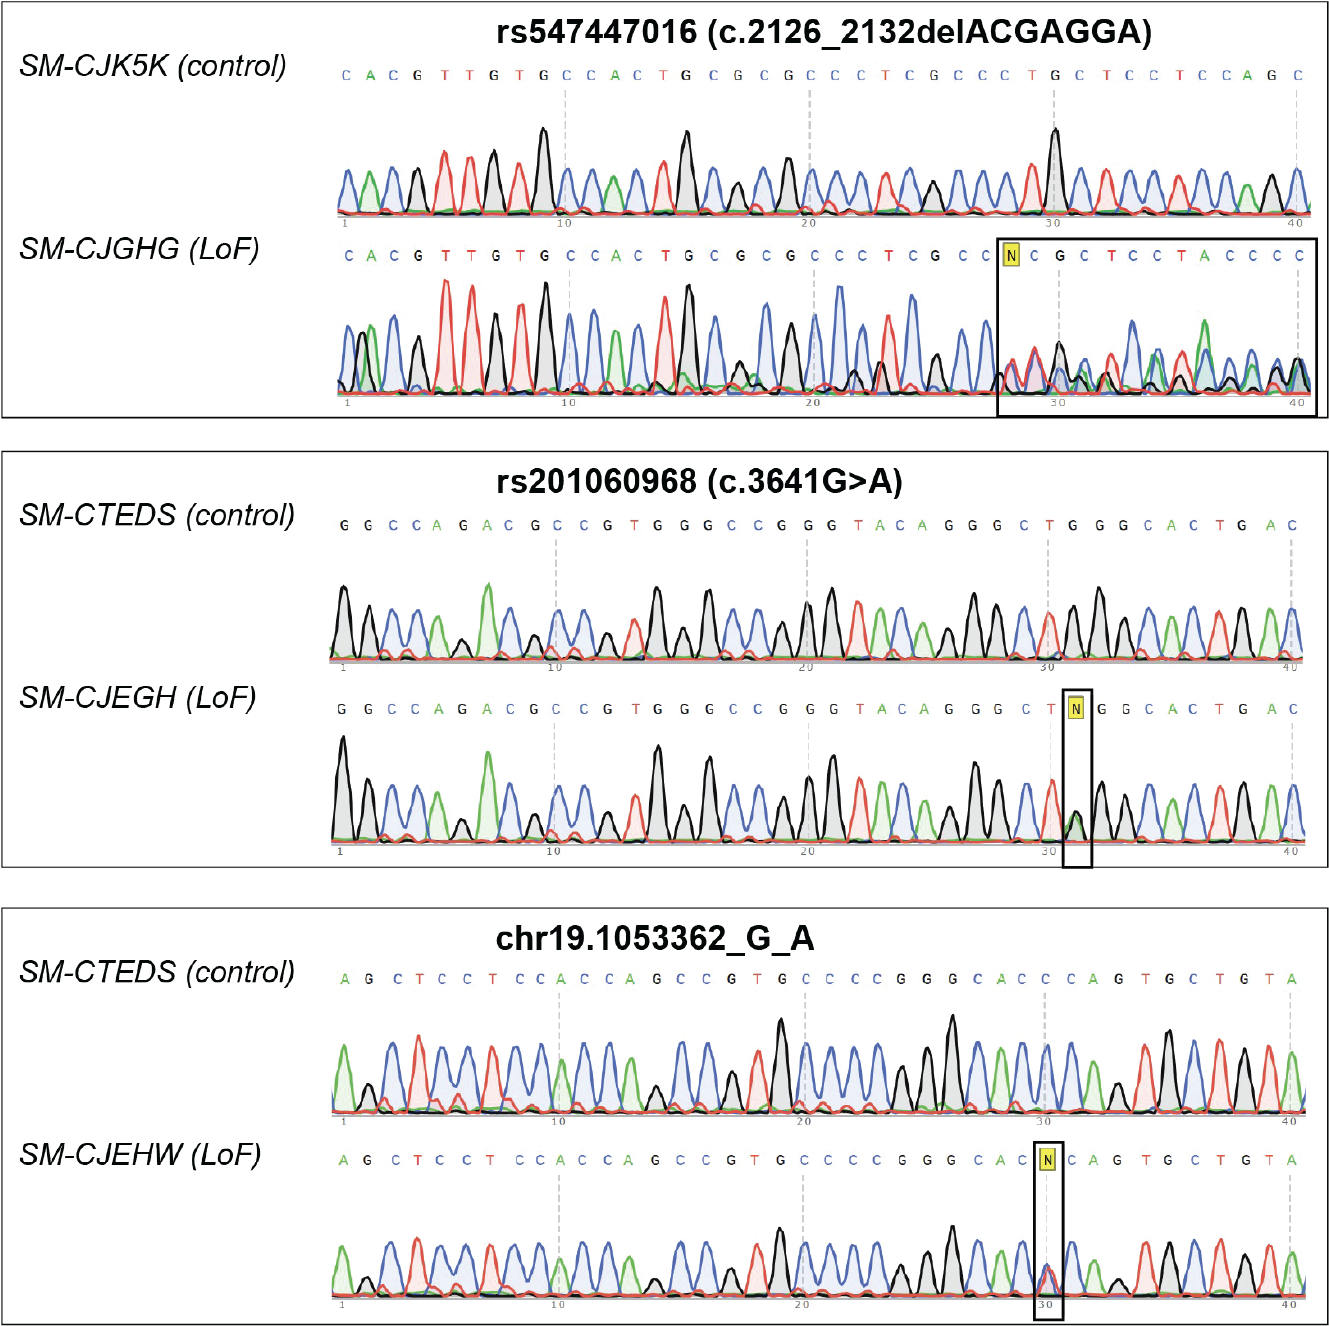
\includegraphics[width=\textwidth]{./extended_plots/sanger_seq.png}        
    \end{subfigure}  
    \begin{subfigure}[t]{.5\textwidth}
        \begin{subfigure}[t]{\textwidth}
            \caption{}
            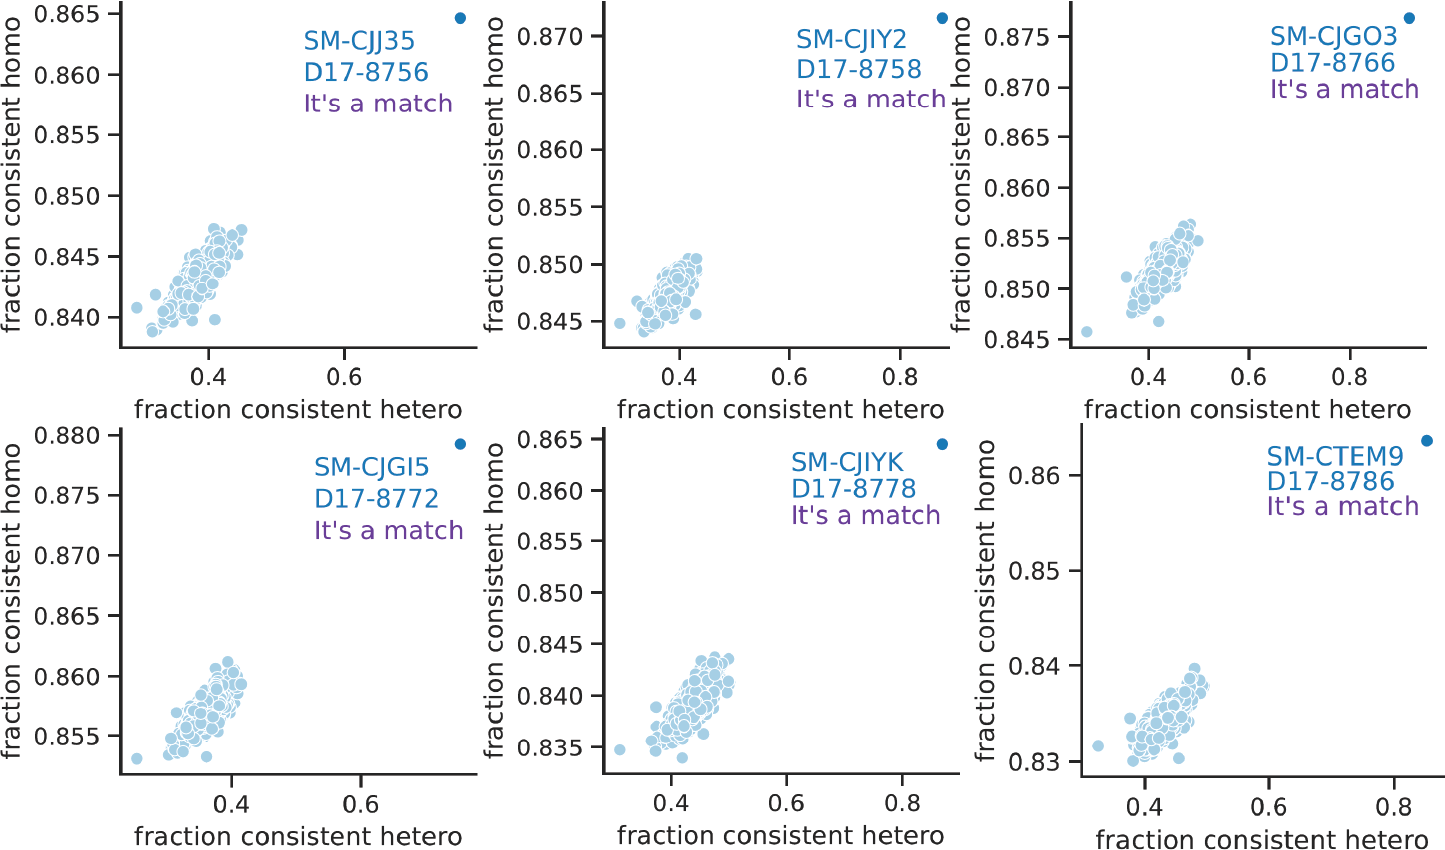
\includegraphics[width=\textwidth]{./extended_plots/sample_swap.png}        
        \end{subfigure}  
        \begin{subfigure}[t]{\textwidth}
            \caption{}
            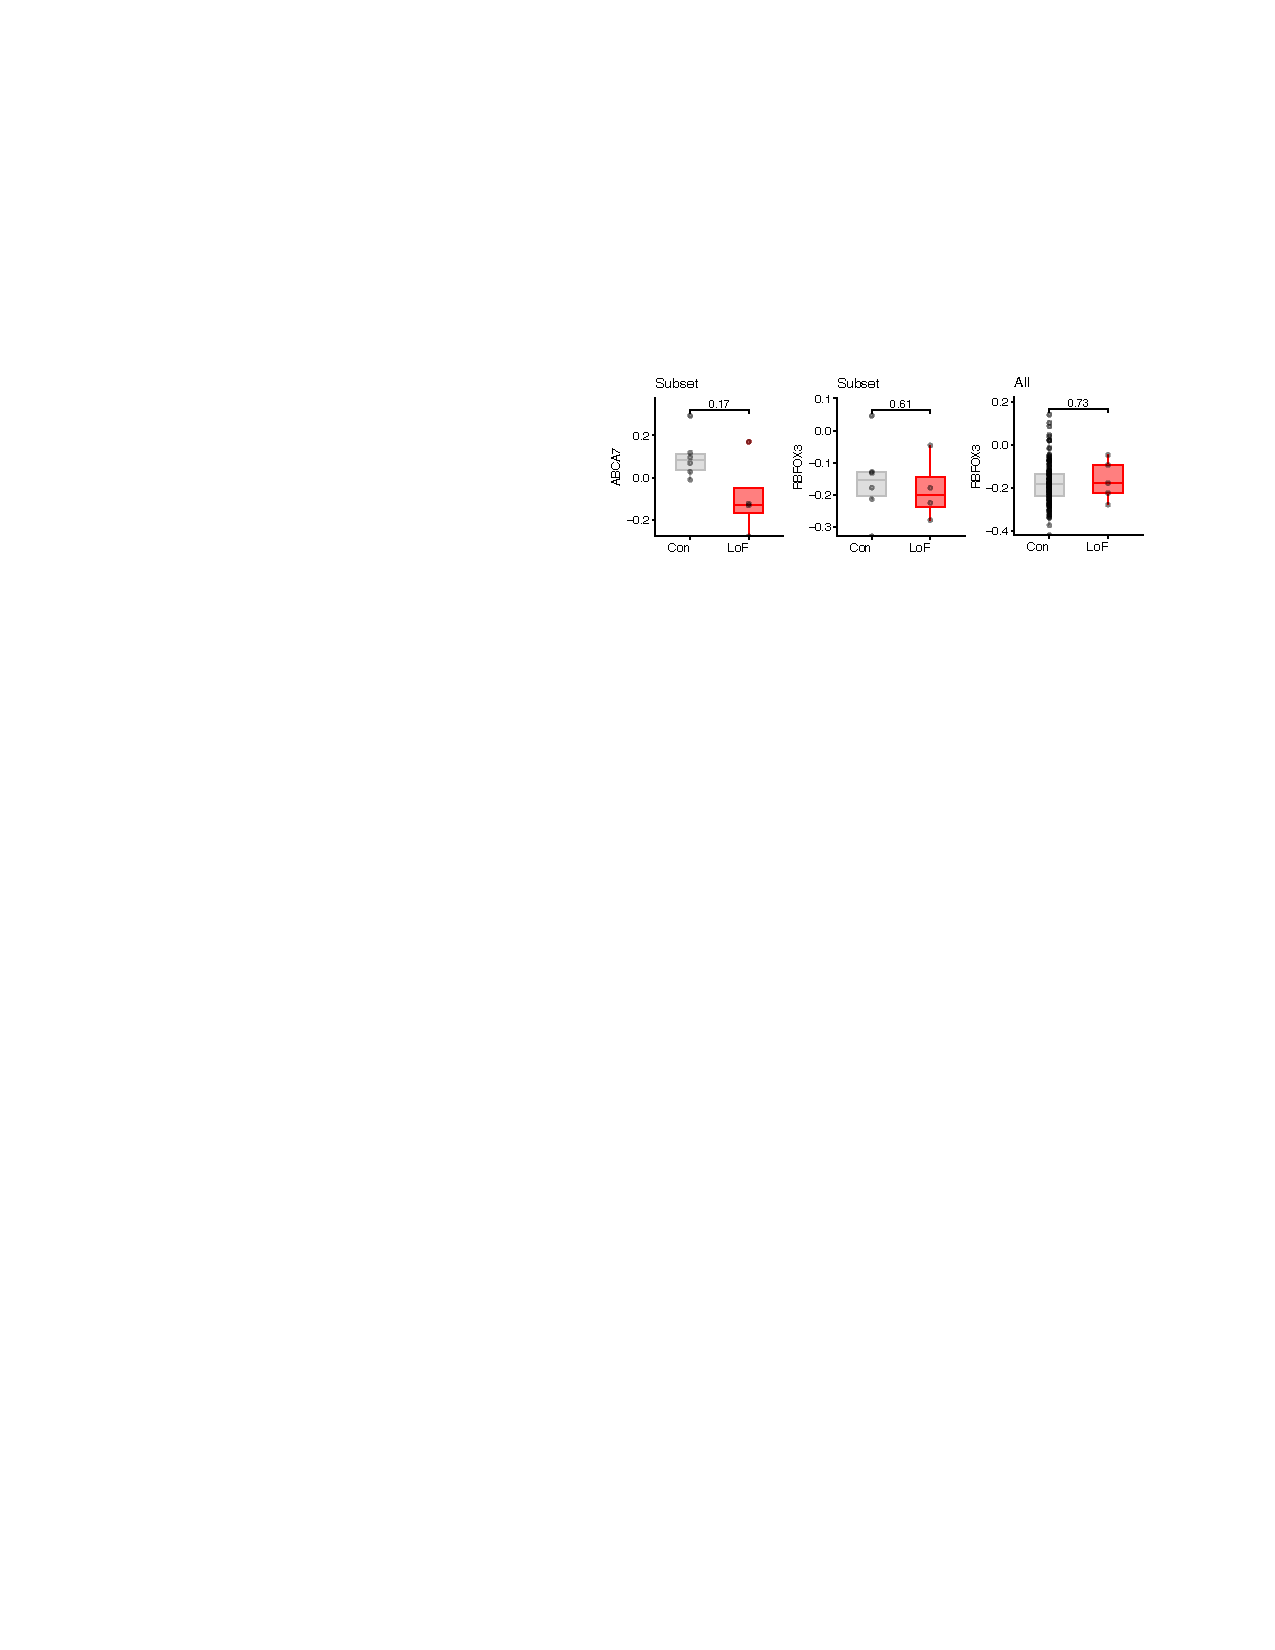
\includegraphics[width=\textwidth]{./extended_plots/protein_levels_extended.pdf}        
        \end{subfigure}  
    \end{subfigure}  
    \begin{subfigure}[t]{\textwidth}
        \caption{}
        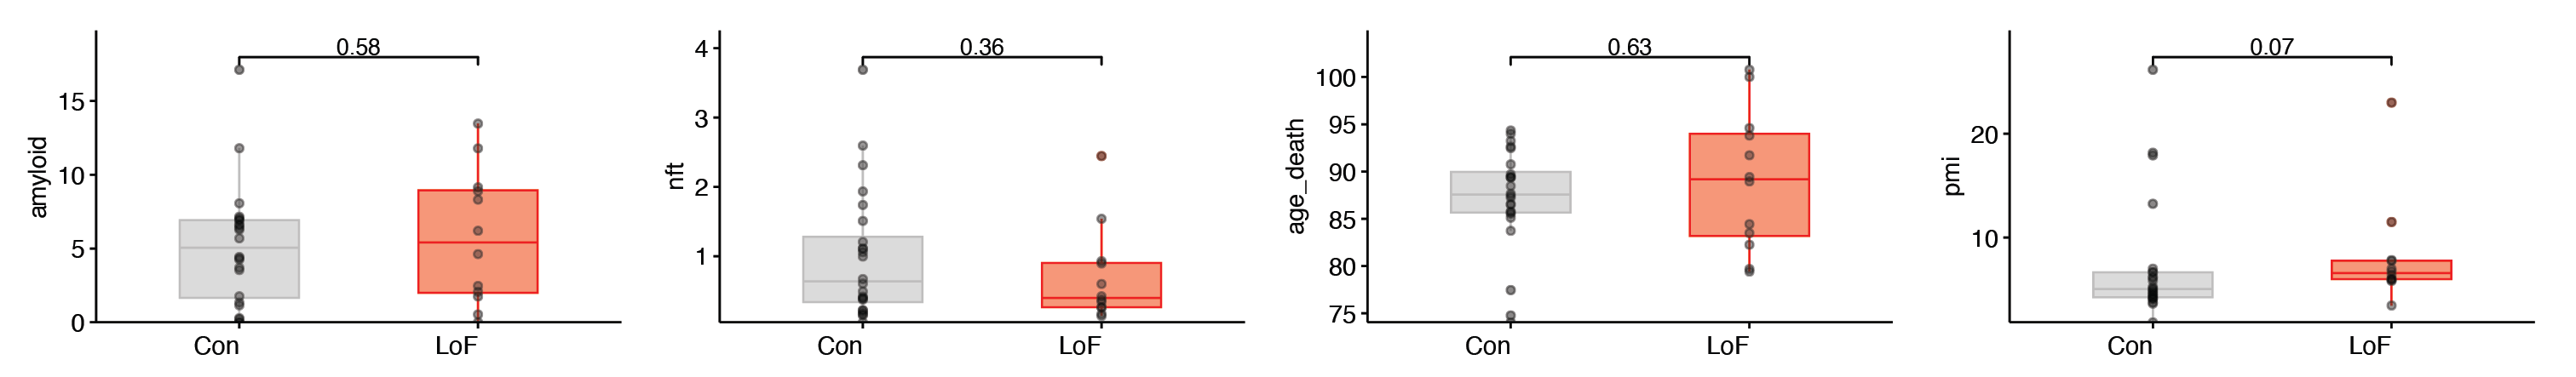
\includegraphics[width=\textwidth]{./extended_plots/batch_cont_var.png}        
    \end{subfigure}  
    \begin{subfigure}[t]{\textwidth}
        \caption{}
        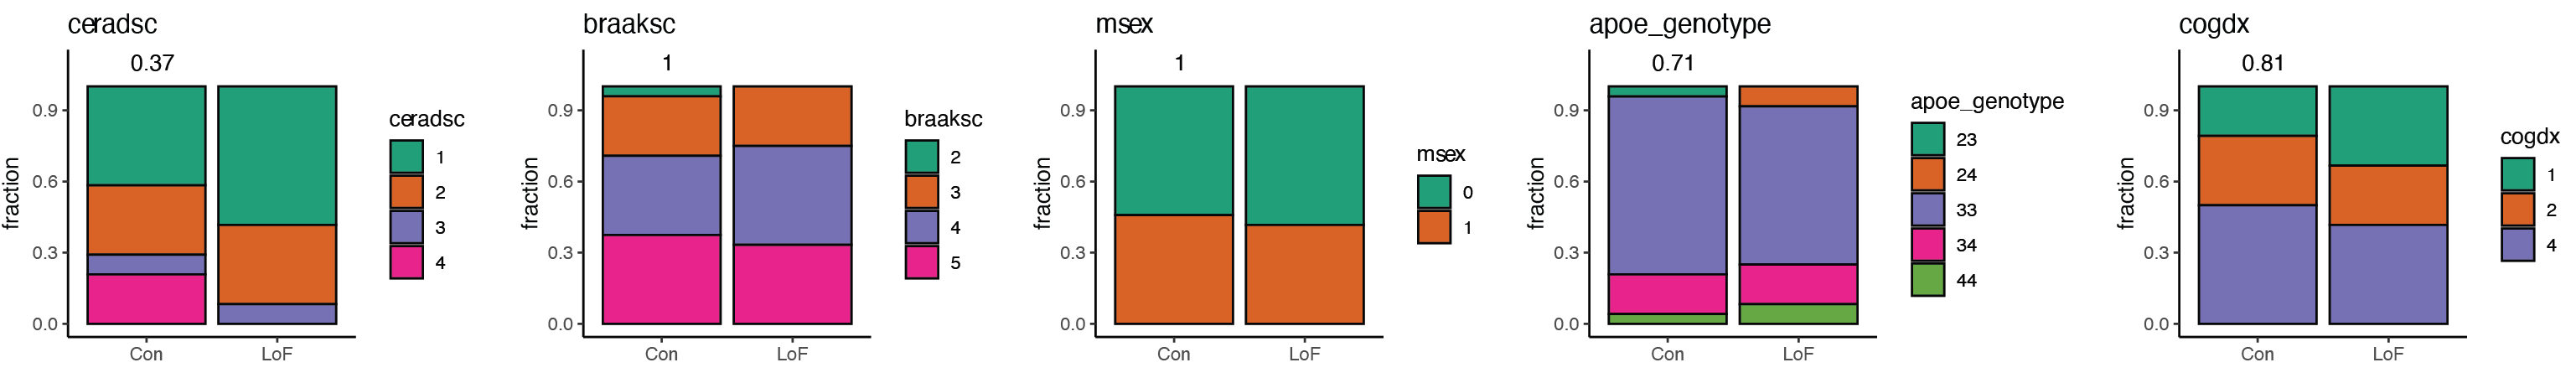
\includegraphics[width=\textwidth]{./extended_plots/batch_categorical_vars.png}        
    \end{subfigure}  
    \caption{
        \textbf{Overview of Human snRNA-Sequencing Cohort.}\\[1ex]
        (A) Sanger sequencing of ABCA7 LoF variants in prefrontal cortex genomic DNA samples from 3 ABCA7 LoF carriers and 3 controls from the snRNA-seq cohort. Sequencing confirmed heterozygosity of the indicated variant in LoF samples, with variant location marked by a black box. 
        (B) Example plots validating matches between whole genome sequencing (WGS) and snRNA-seq libraries. Each plot shows the concordance of homo- and heterozygous SNP calls between WGS and snRNA-seq data for a single individual. Matches between WGS SNP calls and snRNA-seq BAM inferred SNP calls are indicated by extreme outliers. Expected (i.e., correct) matches are indicated in blue/purple. 
        (C) Protein levels from post-mortem human prefrontal cortex (see Table~\ref{tab:external_datasets} for external dataset used) showing ABCA7 protein levels (left) and NeuN (RBFOX3) levels (middle) for a subset of individuals in the snRNA-seq cohort (N=6 control and N=4 ABCA7 LoF carriers). The right panel shows NeuN (RBFOX3) protein levels by genotype in all available control samples (N=180) vs. ABCA7 LoF carriers (N=5). 
        (D) Distributions of continuous metadata variables (see Supplementary Text for descriptions) for control individuals (N=24) vs. ABCA7 LoF carriers (N=12). For panels C and D, boxes indicate dataset quartiles per condition, and whiskers extend to the most extreme data points not considered outliers (i.e., within 1.5 times the interquartile range from the first or third quartile). 
        (E) Distributions of discrete metadata variables for control individuals (N=24) vs. ABCA7 LoF carriers (N=12). Con=control, LoF=ABCA7 loss-of-function. P-values in panels C and D were computed by two-sided Wilcoxon rank sum test. P-values in panel E were computed by two-sided Fisher’s exact test.
    }
    \label{fig:snRNA_cohort}
\end{figure}
\clearpage
% Batch quality
\begin{figure}[H]
    \begin{subfigure}[t]{\textwidth}
        \caption{}
        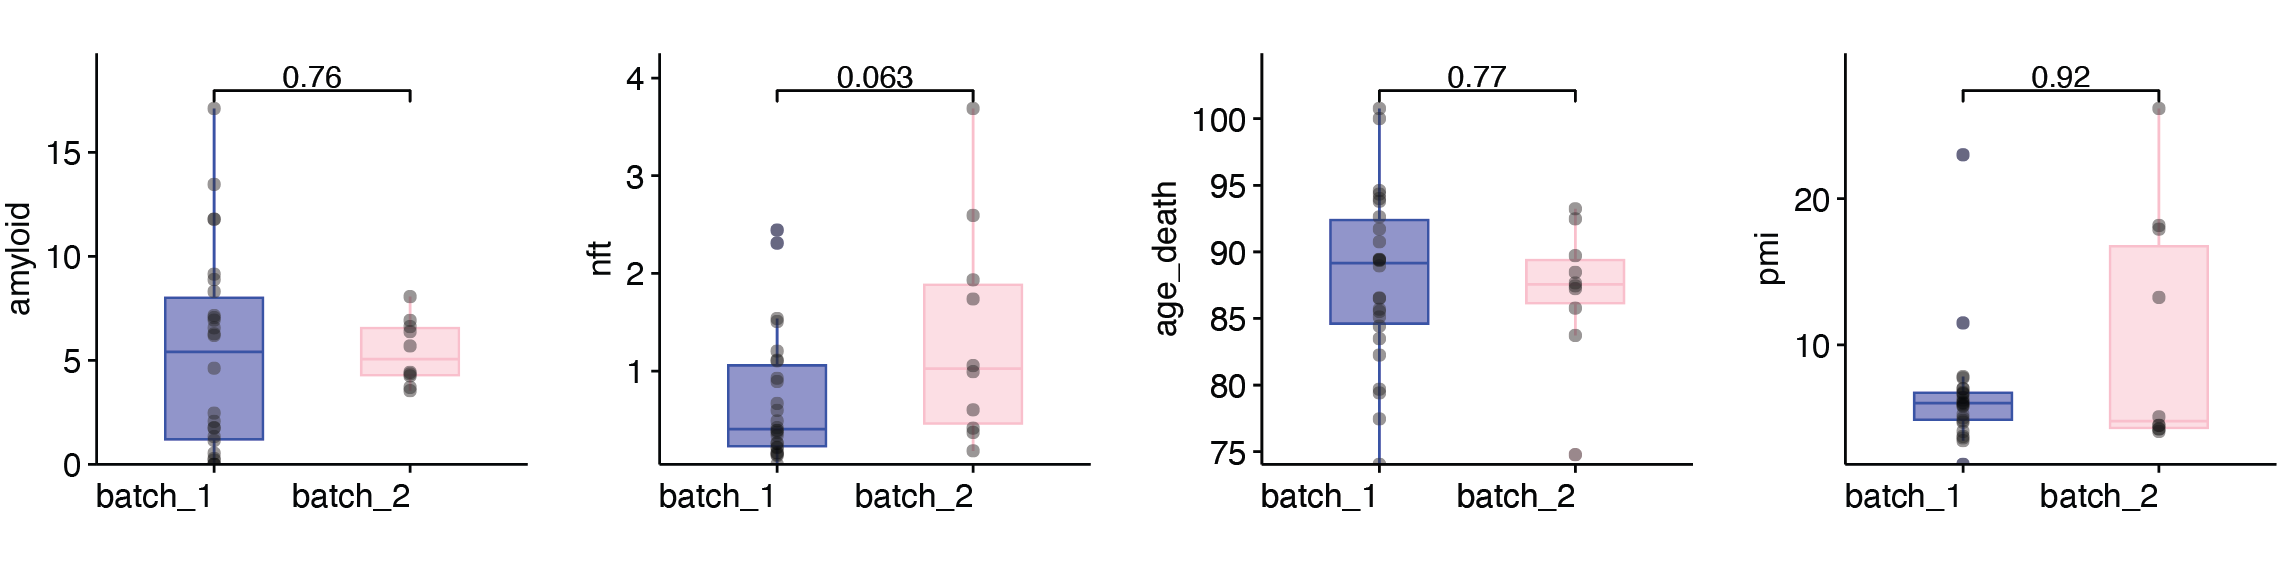
\includegraphics[width=\textwidth]{./extended_plots/seq_batch_cont.png}        
    \end{subfigure}
    \begin{subfigure}[t]{\textwidth}
        \caption{}
        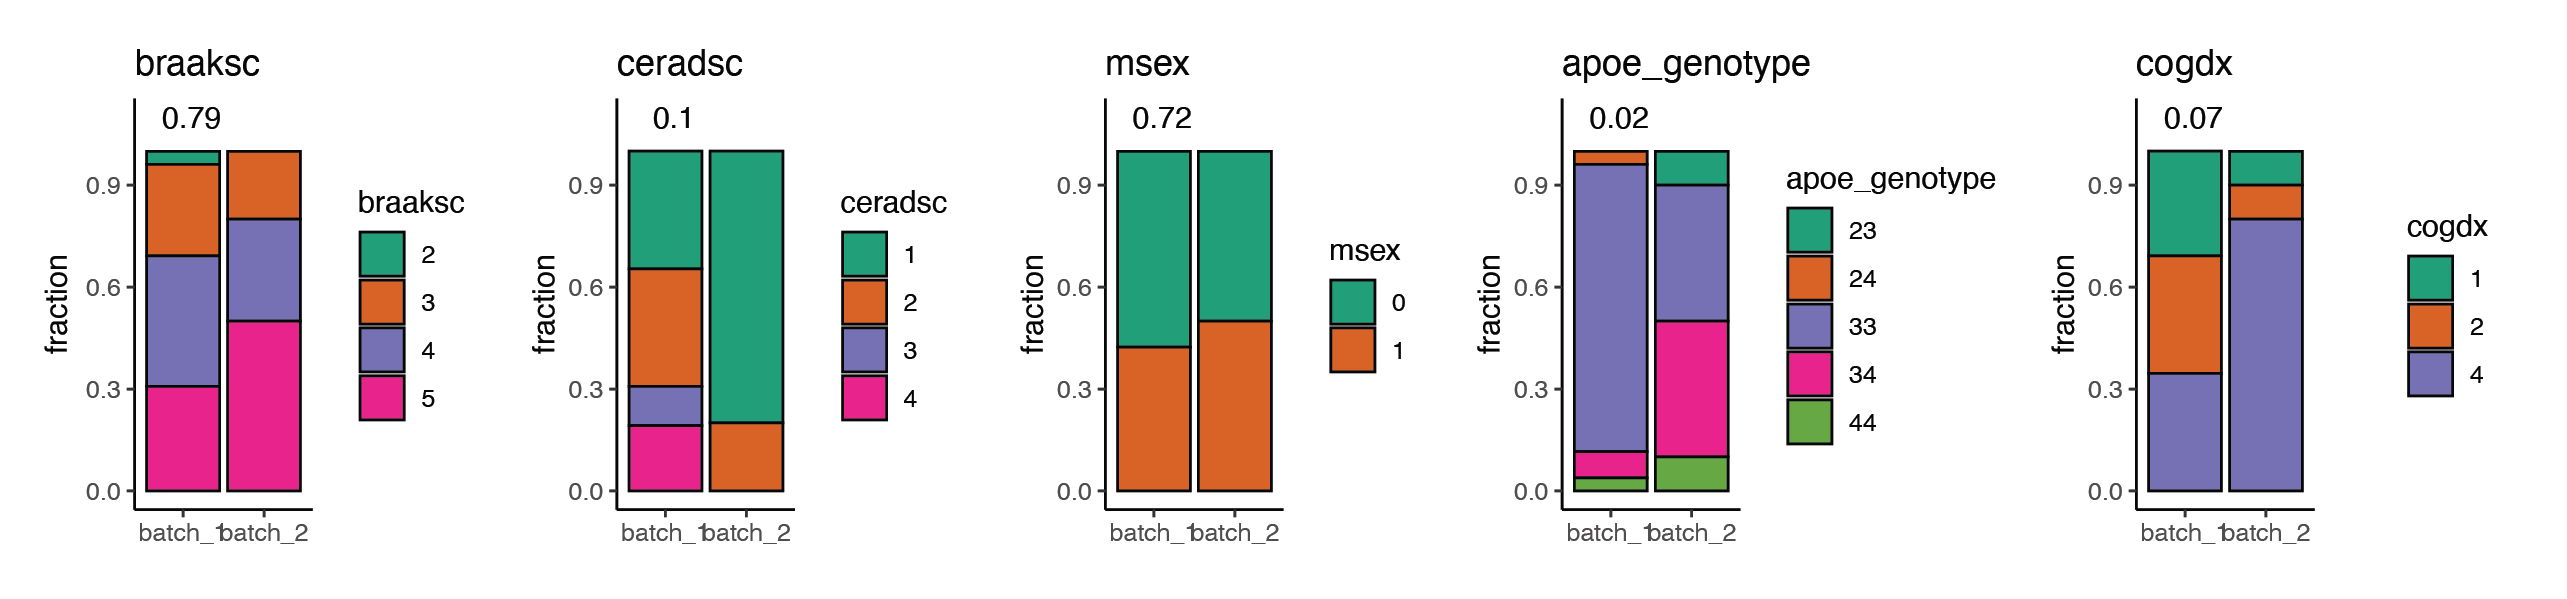
\includegraphics[width=\textwidth]{./extended_plots/seq_batch_cat.png}        
    \end{subfigure}  
    \begin{subfigure}[t]{\textwidth}
        \caption{}
        \includegraphics[width=\textwidth]{./extended_plots/additional_projections.png}        
    \end{subfigure}   
    \caption{
        \textbf{Overview of snRNA-sequencing Batch Correction and Data Quality.}\\
    }
    \label{fig:snRNA_quality_annotation}
\end{figure}
\begin{itemize}
    \item[\textbf{(A,B)}] Distributions of continuous (A) and discrete (B) metadata variables by sequencing batch. 
    \item[\textbf{(C)}] Two-dimensional UMAP projection of snRNA-seq single cells from gene expression space, colored by selected variables after all rounds of quality control. 
\end{itemize}
\clearpage
% Annotation
\begin{figure}[H]
    \begin{subfigure}[t]{.5\textwidth}
        \begin{subfigure}[t]{.45\textwidth}
            \caption{}
            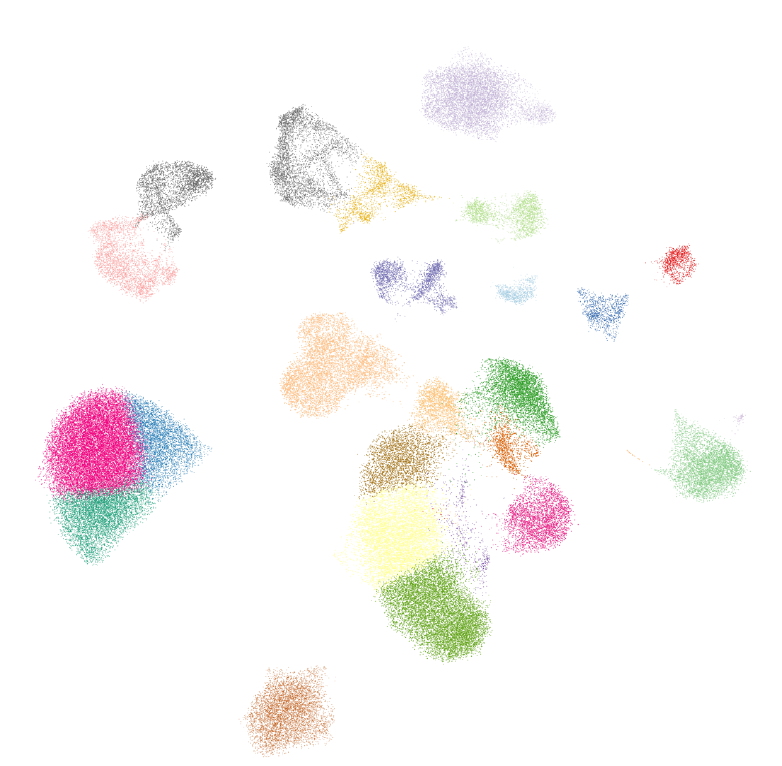
\includegraphics[width=\textwidth]{./extended_plots/cell_proj_with_leiden.png}        
        \end{subfigure}
        \hspace{0.5cm}  
        \begin{subfigure}[t]{.45\textwidth}
            \caption{}
            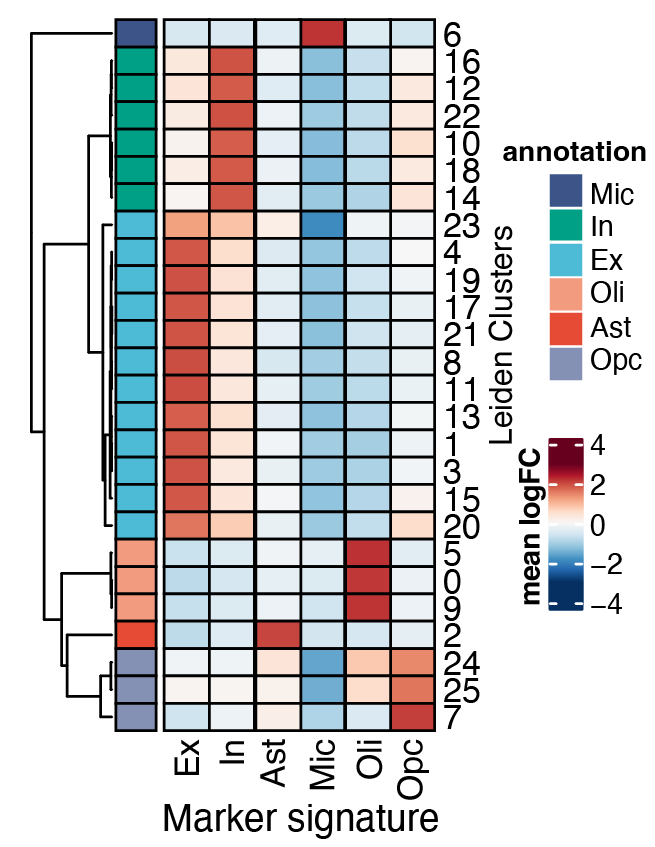
\includegraphics[width=\textwidth]{./extended_plots/leiden_heatmap.png}        
        \end{subfigure}   
        \begin{subfigure}[t]{.3\textwidth}
            \caption{}
            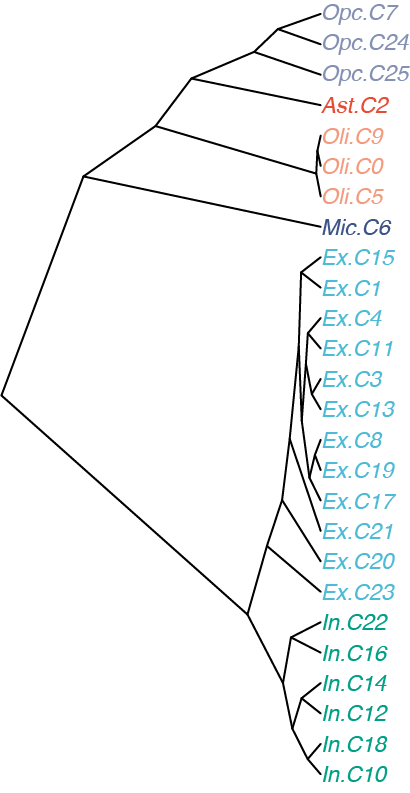
\includegraphics[width=\textwidth]{./extended_plots/hierarchical_tree.png}        
        \end{subfigure}  
        \hspace{1cm}
        \begin{subfigure}[t]{.45\textwidth}
            \caption{}
            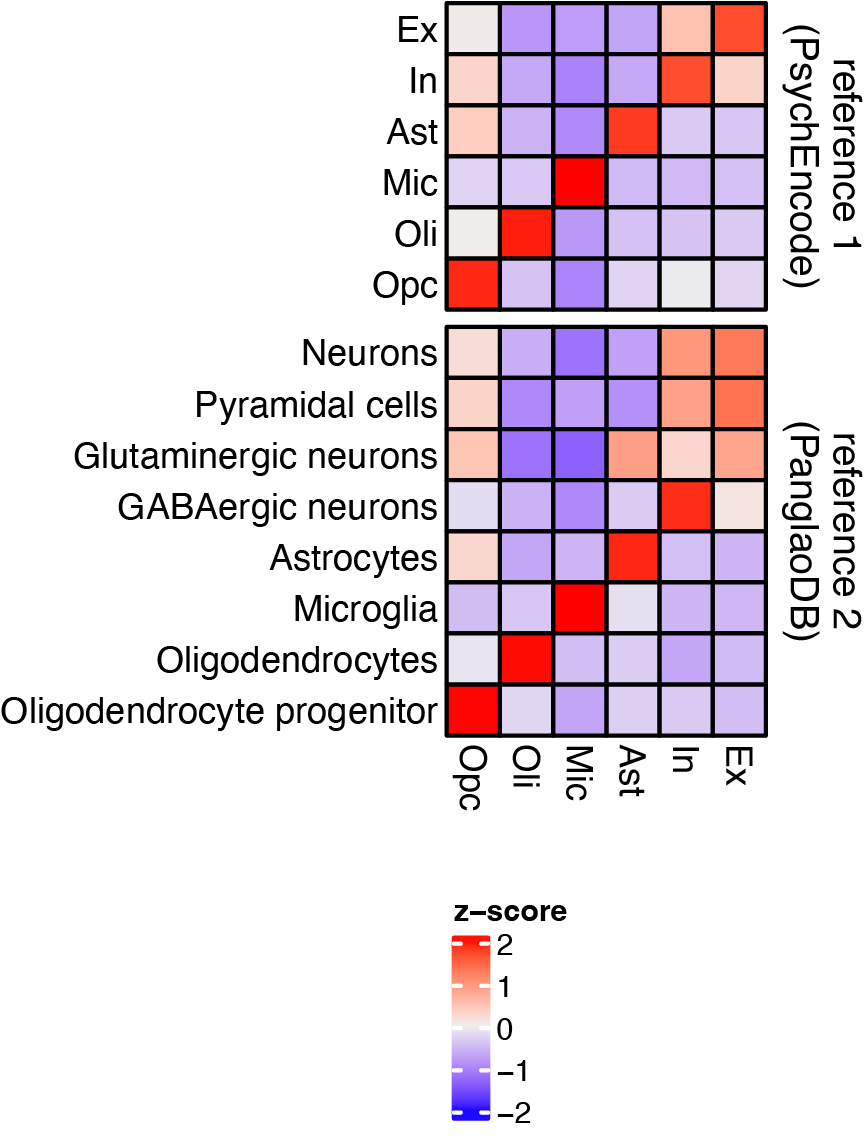
\includegraphics[width=\textwidth]{./extended_plots/marker_hmap.png}        
        \end{subfigure}  
    \end{subfigure}
    \hspace{2cm}  
    \begin{subfigure}[t]{.25\textwidth}
        \caption{}
        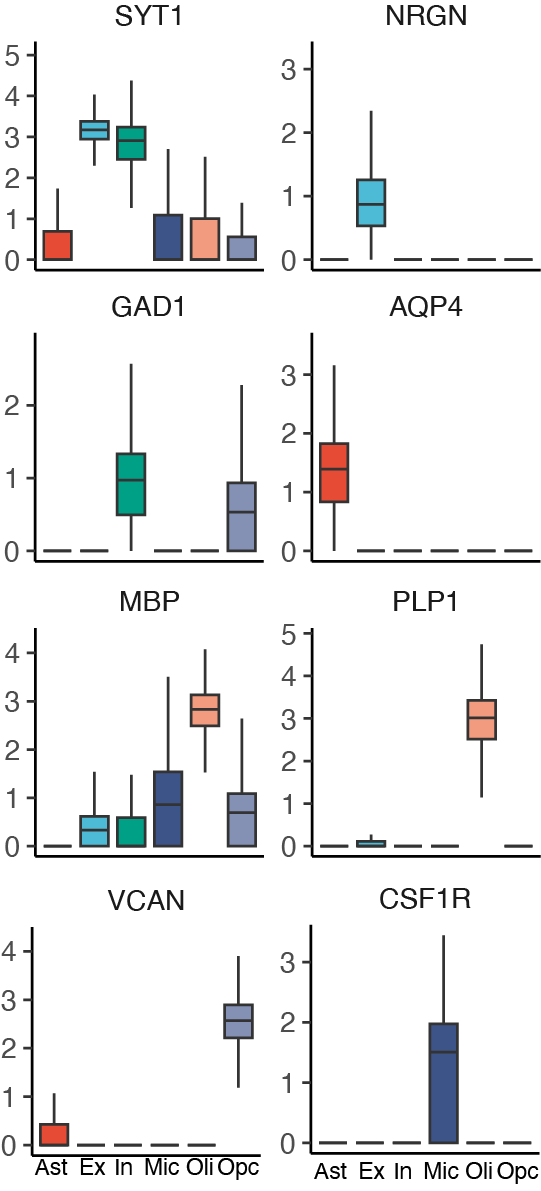
\includegraphics[width=\textwidth]{./extended_plots/marker_boxplot.png}        
    \end{subfigure}    
    \par
    \begin{subfigure}[t]{.15\textwidth}
        \caption{}
        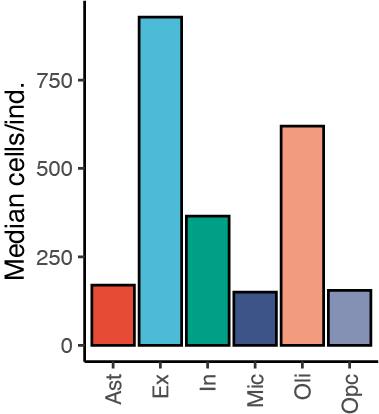
\includegraphics[width=\textwidth]{./extended_plots/median_cells.png}        
    \end{subfigure} 
    \hspace{0.5cm}   
    \begin{subfigure}[t]{.25\textwidth}
        \caption{}
        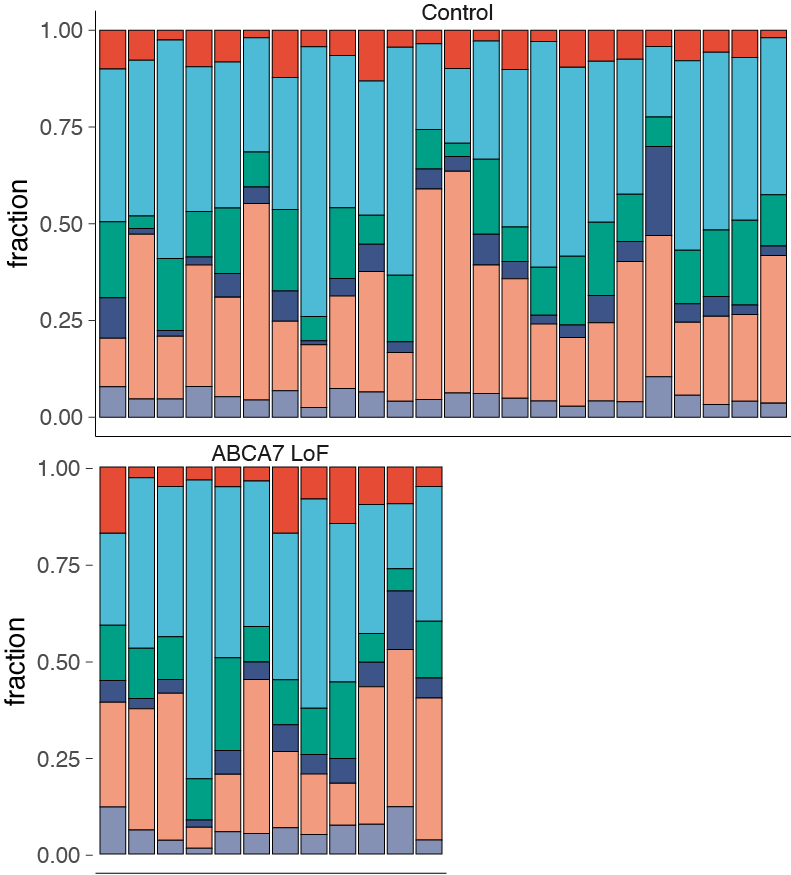
\includegraphics[width=\textwidth]{./extended_plots/individual_fractions.png}        
    \end{subfigure}  
    \hspace{0.5cm}   
    \begin{subfigure}[t]{.25\textwidth}
        \caption{}
        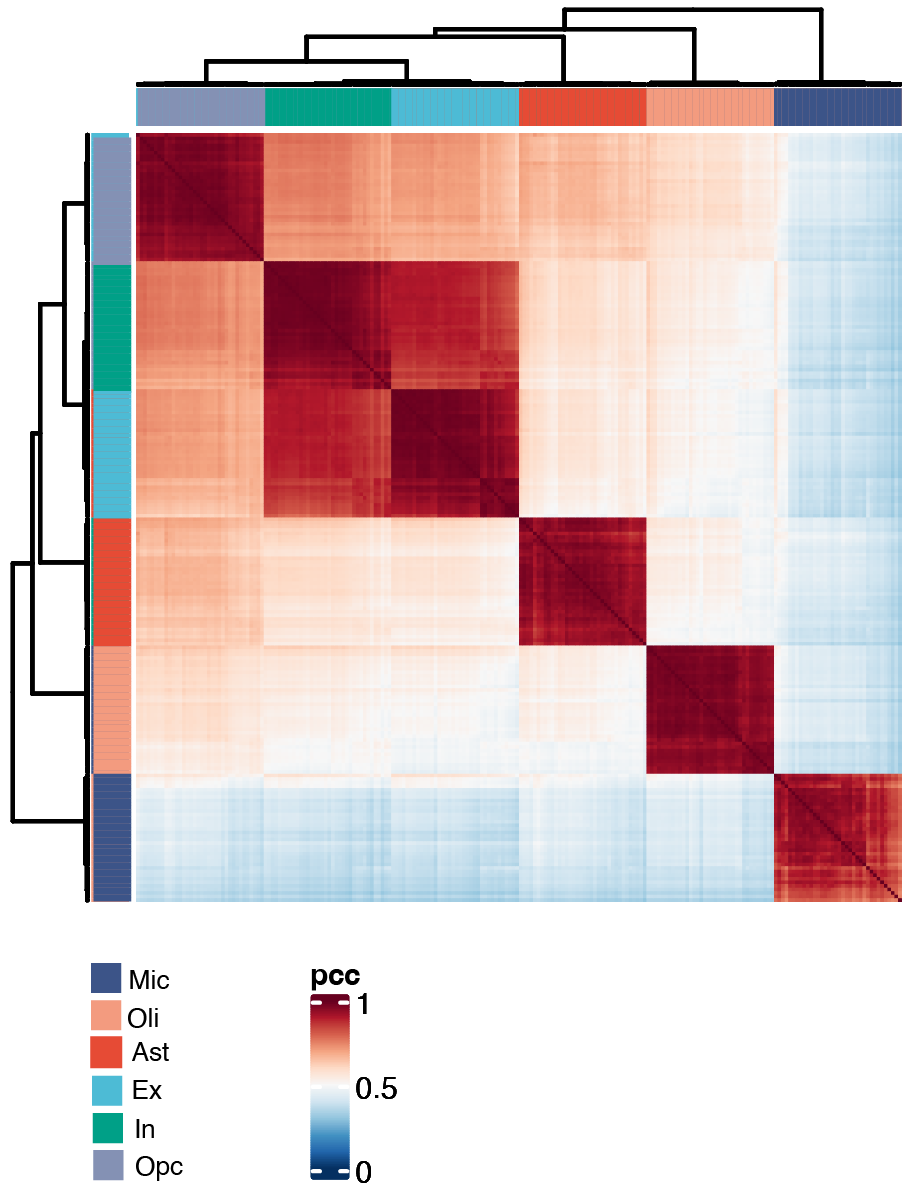
\includegraphics[width=\textwidth]{./extended_plots/celltype_heatmap.png}        
    \end{subfigure}  
    \hspace{0.5cm}
    \begin{subfigure}[t]{.15\textwidth}
        \caption{}
        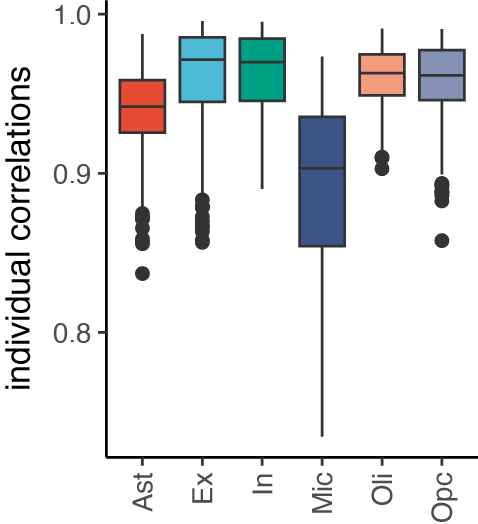
\includegraphics[width=\textwidth]{./extended_plots/individual_correlations.png}        
    \end{subfigure}       
    \caption{
        \textbf{Overview of snRNA-sequencing Cell Type Annotations.}\\
    }
    \label{fig:snRNA_quality_annotation}
\end{figure}
\begin{itemize}
    \item[\textbf{(A)}] Two-dimensional UMAP projections of individual cells from gene expression space, colored by Leiden clusters. 
    \item[\textbf{(B)}] Average marker gene expression (per-cluster mean log(fold-change)) for all marker genes for the cell type indicated along the x-axis. Log(fold-changes) are computed for the cluster of interest vs. all remaining clusters. Reference 1 (Table 2) marker genes were used. 
    \item[\textbf{(C)}] Cladogram visualizing subcluster relationships based on pairwise distances between per-cluster gene expression profiles. 
    \item[\textbf{(D)}] Average marker gene expression profiles (x-axis) per major cell type annotation (y-axis) for two marker gene references. 
    \item[\textbf{(E)}] Per-cell distribution of select marker gene expression by cell type. Y-axis indicates log counts. 
    \item[\textbf{(F)}] Median number of cells per cell type per individual. 
    \item[\textbf{(G)}] Cell type fraction by individual. 
    \item[\textbf{(H)}] Heatmap of individual-level gene expression correlations by cell type. 
    \item[\textbf{(I)}] Boxplot of individual-level gene expression correlations by cell type. 
\end{itemize}
For all panels, p-values for all continuous variables were computed by two-sided Wilcoxon rank sum test. 
P-values for all discrete variables were computed by two-sided Fisher’s exact test. 
For A, I, M boxes indicate per-condition dataset quartiles, and whiskers extend to the most extreme data points not considered outliers (i.e., within 1.5 times the interquartile range from the first or third quartile).
\clearpage
% Gene scores
\begin{figure}[H]
    \begin{subfigure}[t]{1\textwidth}
        \caption{}
        \centering
        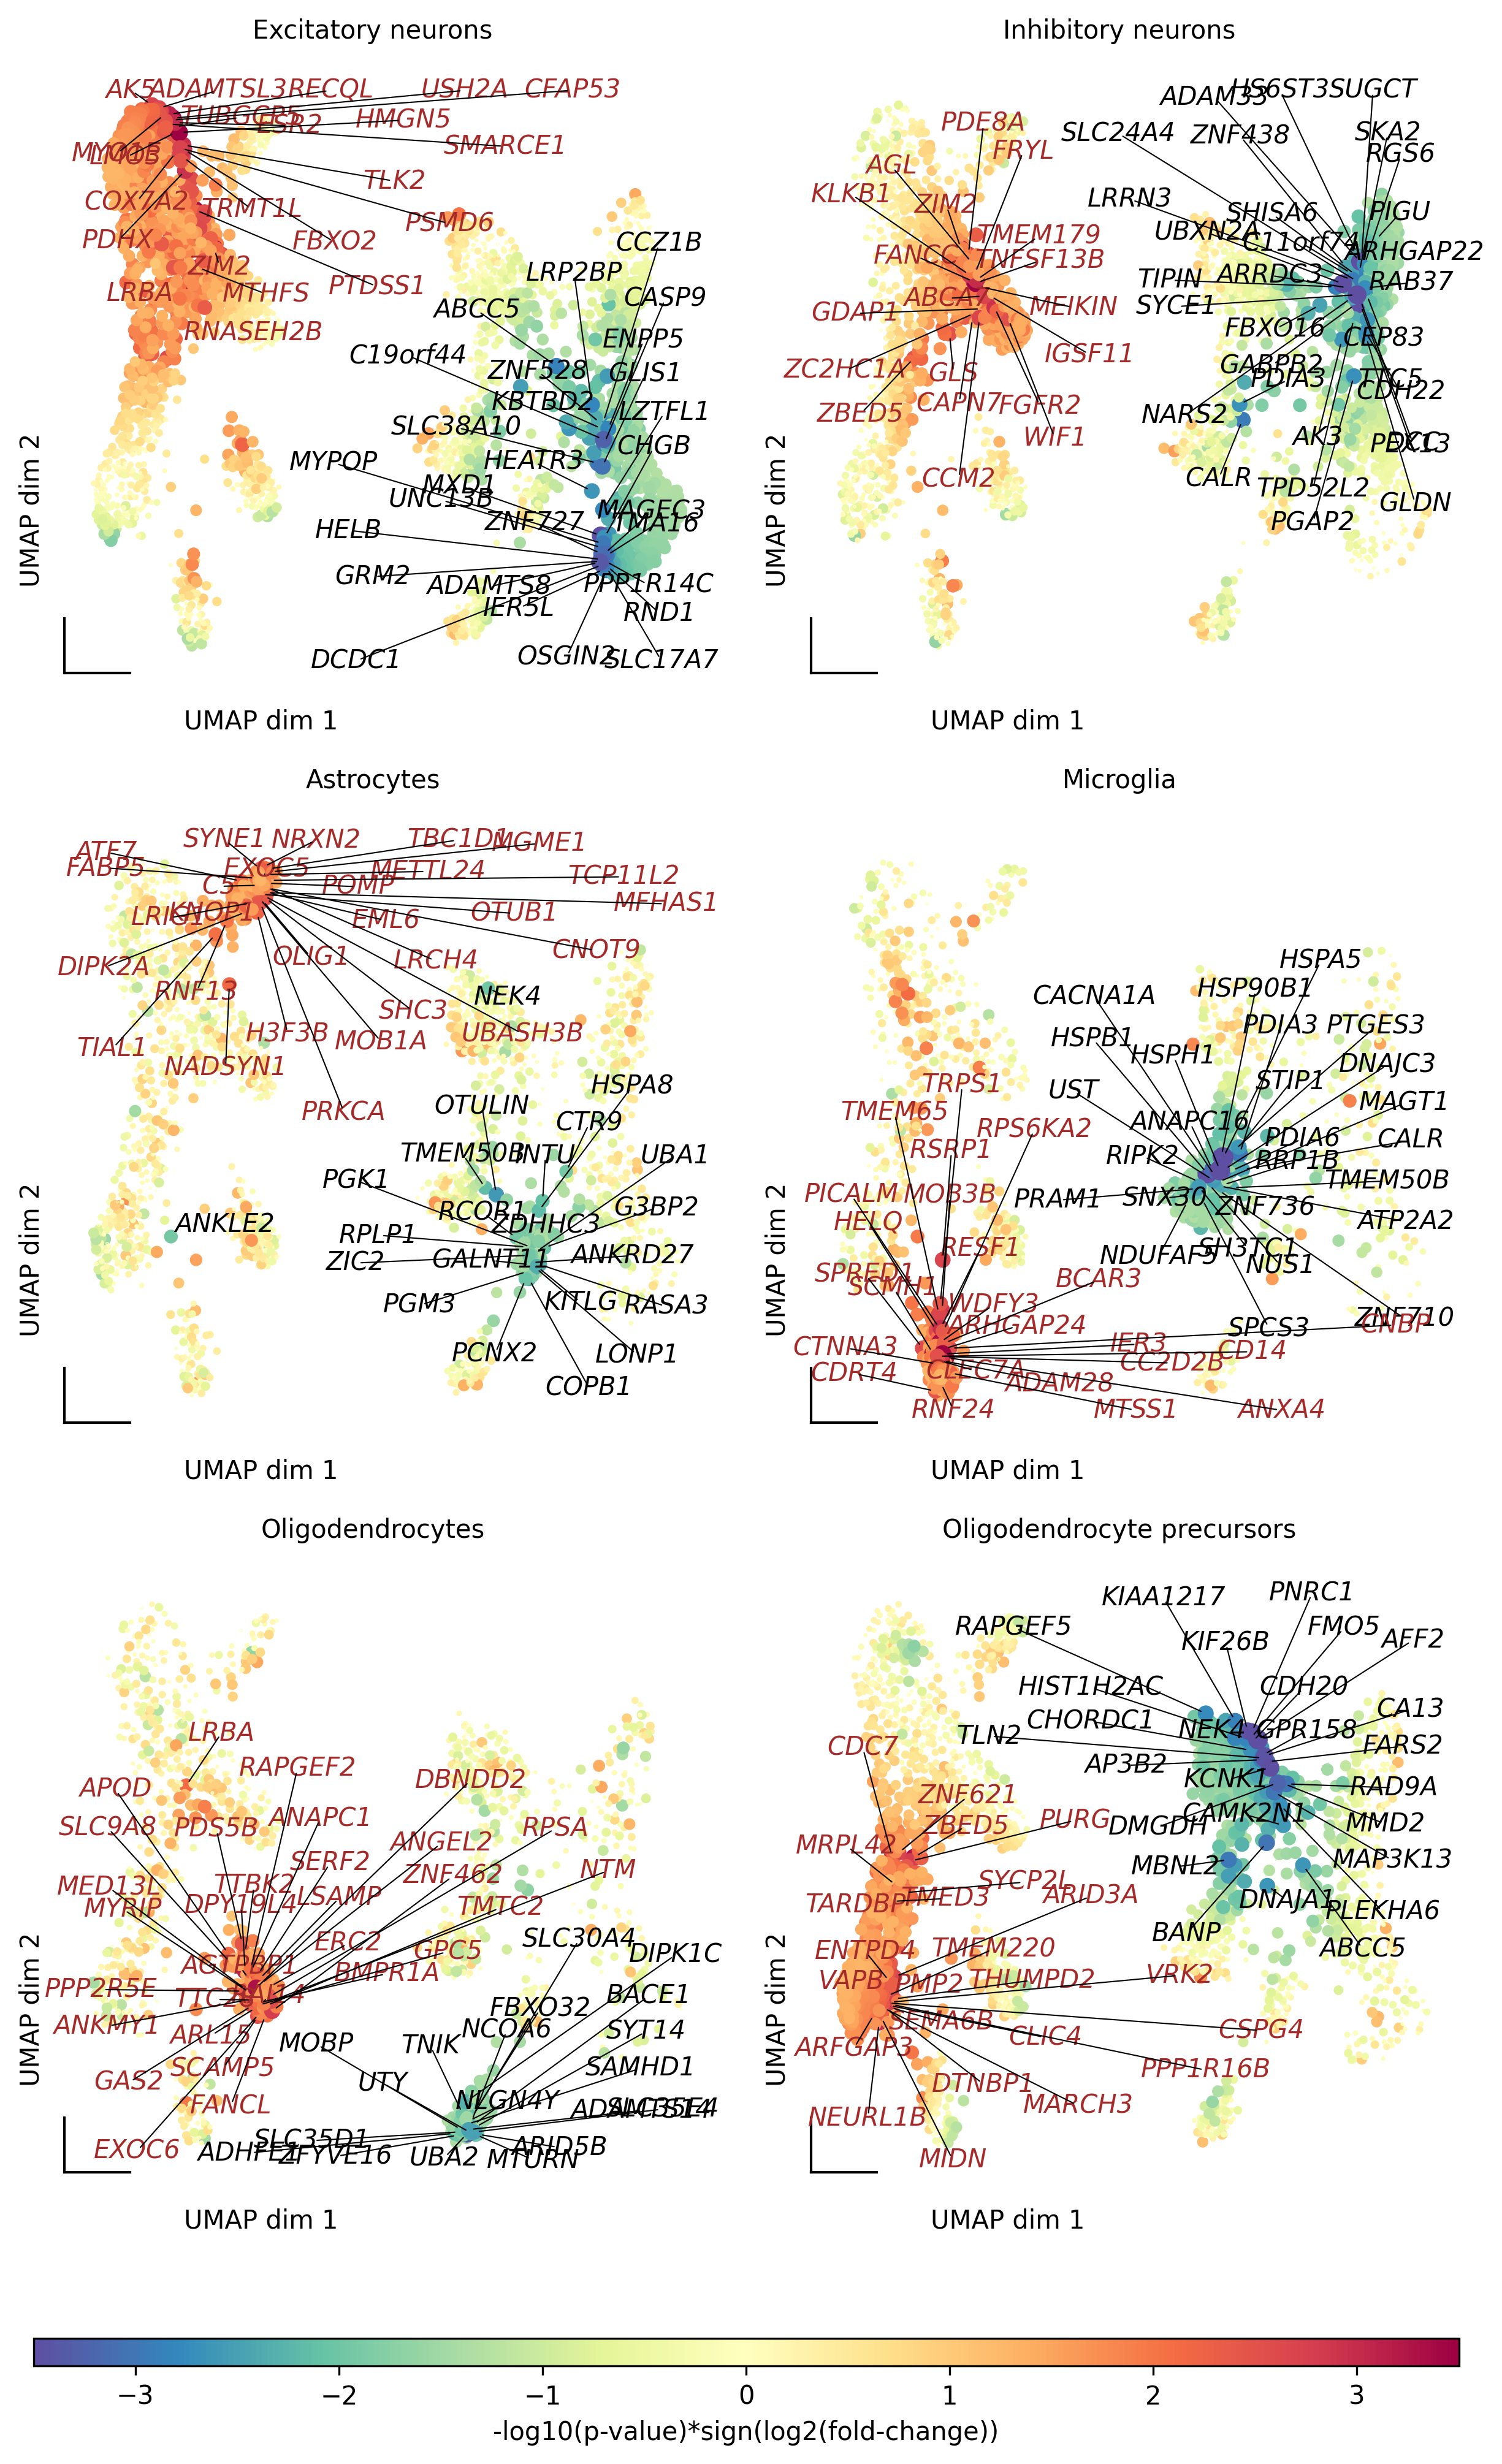
\includegraphics[width=0.7\textwidth]{./extended_plots/umap_projection_more_genes.png}        
    \end{subfigure}    
    \caption{
        \textbf{Annotated projections of gene scores.}\\
    }
    \label{fig:snRNAseq_gene_scores}
\end{figure}

\begin{itemize}
    \item[\textbf{(A)}] Enlarged view of the UMAP projection of Figure~\ref{fig:main_atlas}E, showing the top 20 genes by absolute score ($|S|$) for each cell type. 
\end{itemize}

\clearpage
% ABCA7 expression
\begin{figure}[ht]
    \begin{subfigure}[t]{.3\textwidth}
        \caption{}
        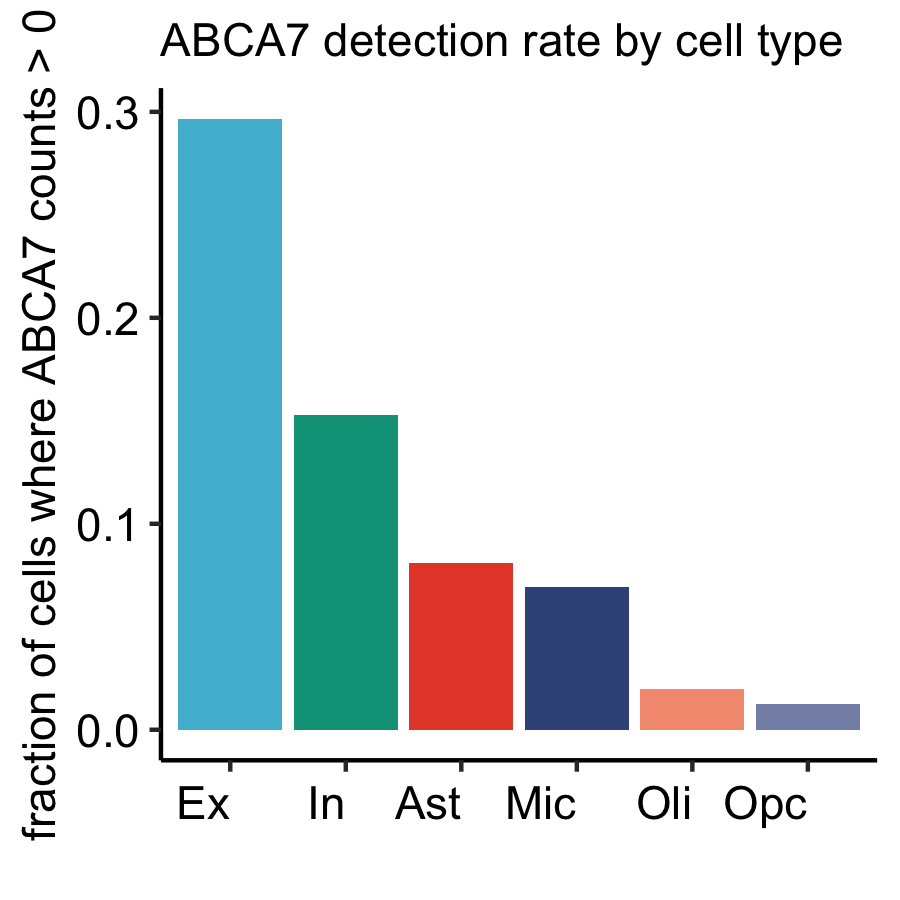
\includegraphics[width=\textwidth]{./extended_plots/abca7_detection_rate.png}        
    \end{subfigure}
    \par
    \begin{subfigure}[t]{1\textwidth}
        \caption{}
        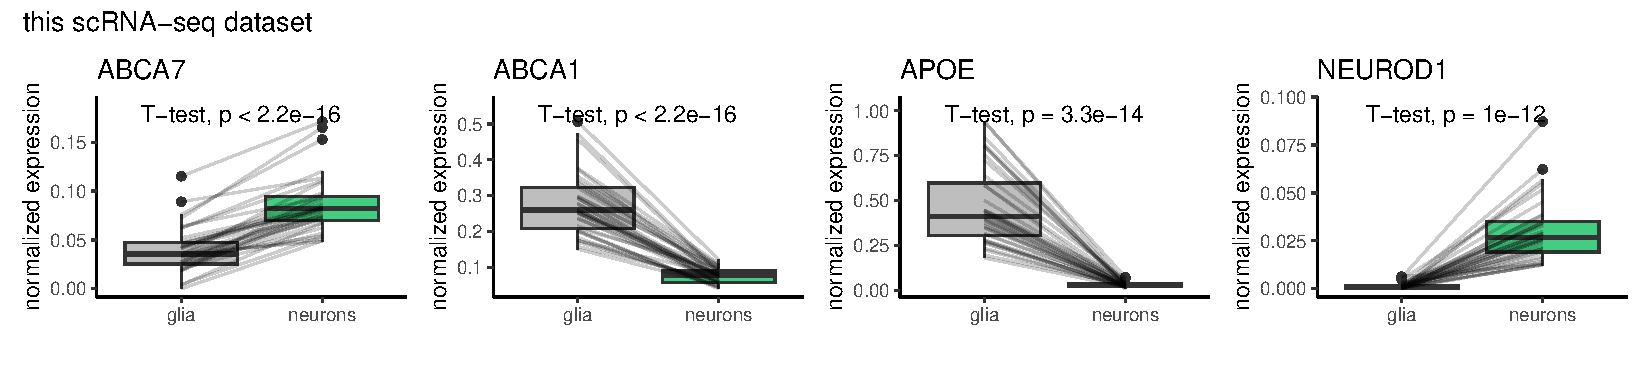
\includegraphics[width=\textwidth]{./extended_plots/scRNAseq_bulk_rna.pdf}        
    \end{subfigure}
    \begin{subfigure}[t]{1\textwidth}
        \caption{}
        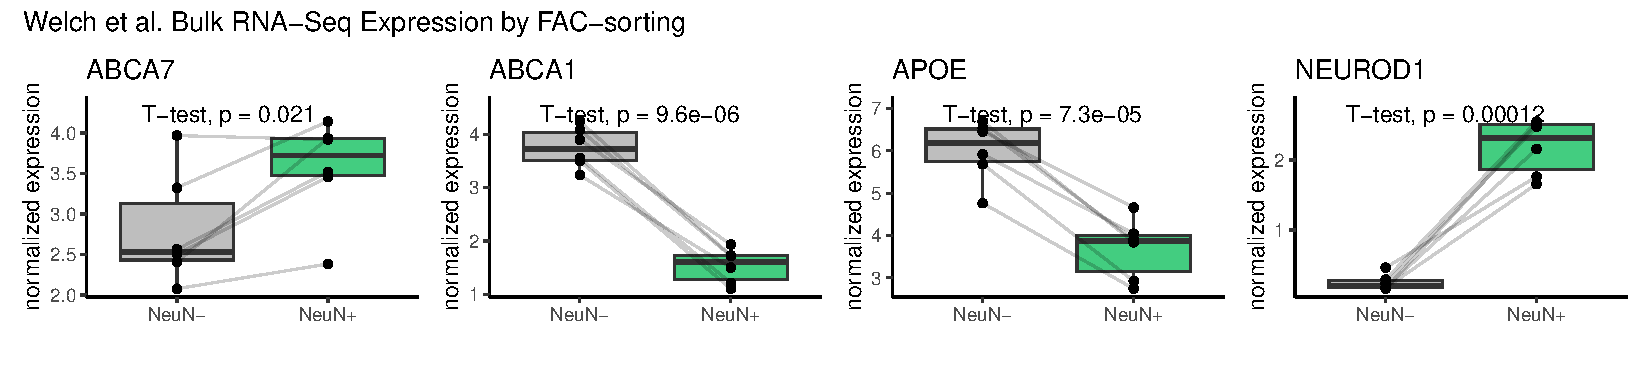
\includegraphics[width=\textwidth]{./extended_plots/welch_et_al_bulk_rna.pdf}        
    \end{subfigure}
    \caption{
        \textbf{Neuronal Expression of ABCA7 in the Post-mortem Human Brain.}\\[1ex]
        (A) Per cell type ABCA7 detection rate of major cell types in the post-mortem PFC as quantified by snRNA-seq. 
        (B) Normalized expression of indicated gene in glial cells (per-individual mean expression profiles across Oli, Opc, Ast, Mic) vs. neuronal cells (per-individual mean expression profiles across Ex and In) from post-mortem snRNA-seq data. 
        (C) Normalized expression of indicated genes in NeuN- vs. NeuN+ cells (N=6 individuals, from \cite{Welch2022-aa}; see Table 2). All p-values are computed by paired two-sided t-test. Boxes indicate per-condition dataset quartiles, and whiskers extend to the most extreme data points not considered outliers (i.e., within 1.5 times the interquartile range from the first or third quartile).
    }
    \label{fig:abca7_expression}
\end{figure}

\clearpage
% Benchmarking clustering
\begin{figure}[ht]
    \begin{subfigure}[t]{0.5\textwidth}
        \caption{}
        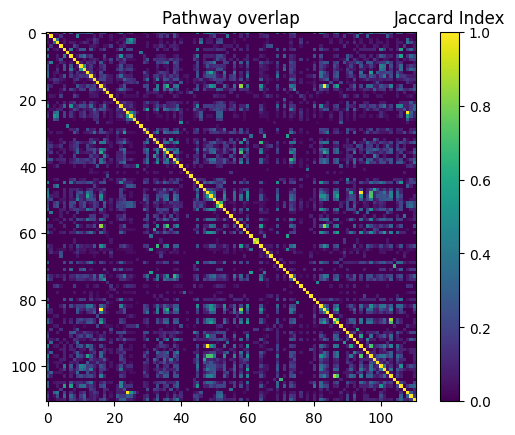
\includegraphics[width=\textwidth]{./extended_plots/jaccard_mat_sub.png}        
    \end{subfigure}
    \begin{subfigure}[t]{0.5\textwidth}
        \caption{}
        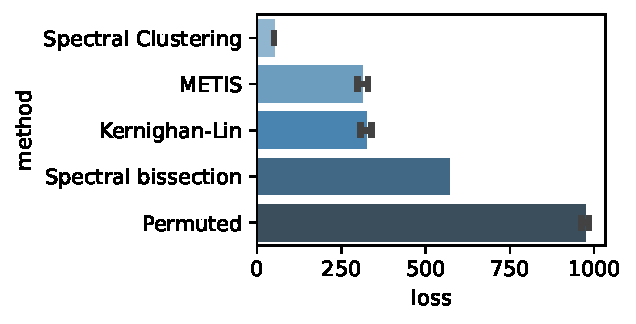
\includegraphics[width=\textwidth]{./extended_plots/partitioning_losses.pdf}        
    \end{subfigure}
    \begin{subfigure}[t]{1\textwidth}
        \caption{}
        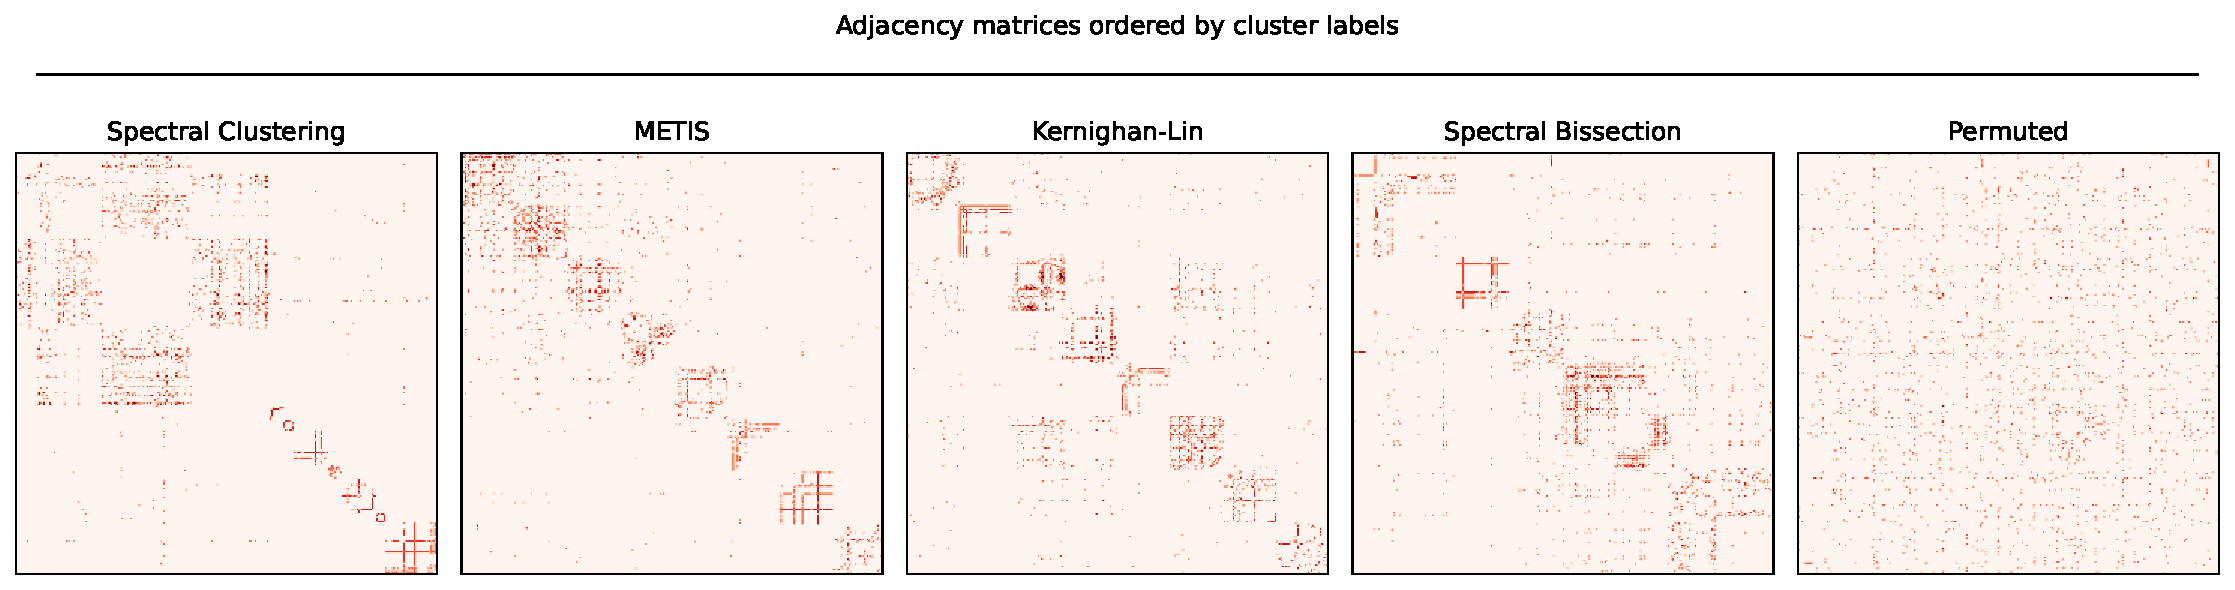
\includegraphics[width=\textwidth]{./extended_plots/adjacency_matrices_ordered_by_cluster_labels.pdf}        
    \end{subfigure}
    \begin{subfigure}[t]{0.33\textwidth}
        \caption{}
        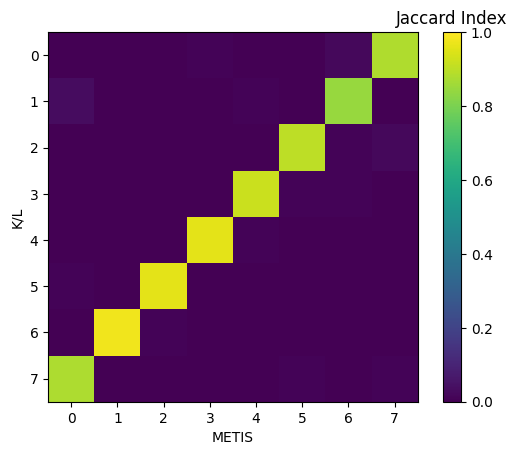
\includegraphics[width=\textwidth]{./extended_plots/argmins_jaccard.png}        
    \end{subfigure}
    \begin{subfigure}[t]{0.33\textwidth}
        \caption{}
        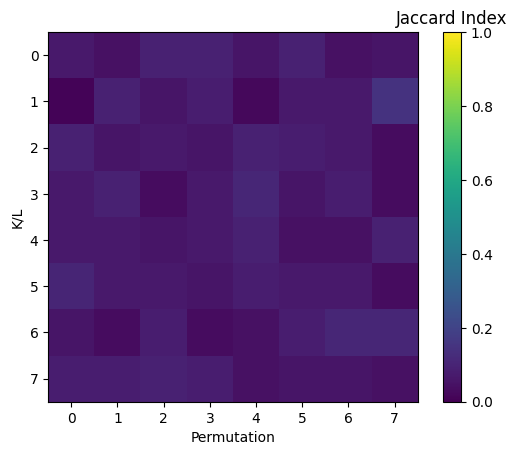
\includegraphics[width=\textwidth]{./extended_plots/random_jaccard.png}        
    \end{subfigure}
    \begin{subfigure}[t]{0.33\textwidth}
        \caption{}
        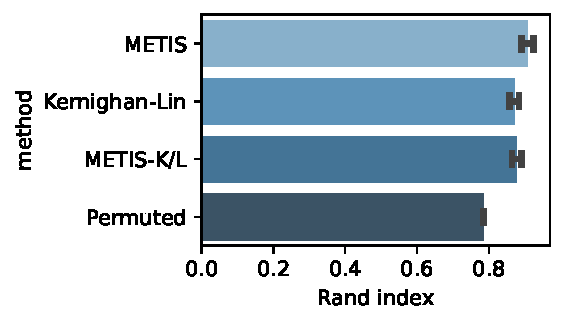
\includegraphics[width=\textwidth]{./extended_plots/rand_indices.pdf}        
    \end{subfigure}
    \caption{
        \textbf{Benchmarking Partitioning and Clustering Algorithms for Gene-Pathway Grouping.}\\[1ex]
        (A) Jaccard indices quantifying overlap of genes for all 111 pathways in Figure~\ref{fig:main_excitatory}B (see Methods; Supplementary Text). 
        (B) Average loss (total cut size; see Methods) associated with applying each algorithm (spectral clustering (SC), METIS, Kernighan-Lin (K/L), spectral bisection (SB), or random permutation) to G (with 379 vertices; see Methods) over 1000 initiations (SC, random permutation) or $5 \times 10^5$ initiations (METIS, K/L). The SB implementation is deterministic and was run only once. Error bars indicate the standard deviation. 
        (C) Unweighted adjacency matrix for G sorted by labels assigned by the indicated algorithm. Red indicates the presence of an edge between two vertices. For each algorithm, labels corresponding to the best initiation (lowest loss) over 1000 initiations (SC, random permutation) or $5 \times 10^5$ initiations (METIS, K/L) are shown. 
        (D) Pairwise labeling consistency for the best K/L initiation and the best METIS initiation. Cluster labels corresponding to each are shown on the X- and Y-axes, respectively. Each color entry indicates the fraction of shared vertices per cluster across two initiations. Consistency is quantified using the Jaccard Index (JI). $\text{JI} = \frac{|A \cap B|}{|A \cup B|}$, where A and B are two sets (i.e., cluster A from initiation \#1 and cluster B from initiation \#2). 
        (E) Same as (D), but comparing the best K/L initiation against the best random permutation initiation. 
        (F) Average Rand index (RI) for all pairwise initiations from (B). “METIS,” “Kernighan-Lin,” and “Permuted” labels on the Y-axis indicate the average RI (consistency across two sets of labels) for all combinations of initiations within the specified algorithm. “METIS-K/L” indicates the average RI for all combinations of initiations across the METIS and Kernighan-Lin algorithms. Error bars indicate standard deviations. ($\text{RI} = \frac{\text{number of agreeing vertex pairs}}{\text{number of vertex pairs}}$).
    }
    \label{fig:benchmarking_clustering}
\end{figure}
\clearpage
% MD simulations
\begin{figure}[H]
    \begin{subfigure}[t]{.4\textwidth}
        \caption{}
        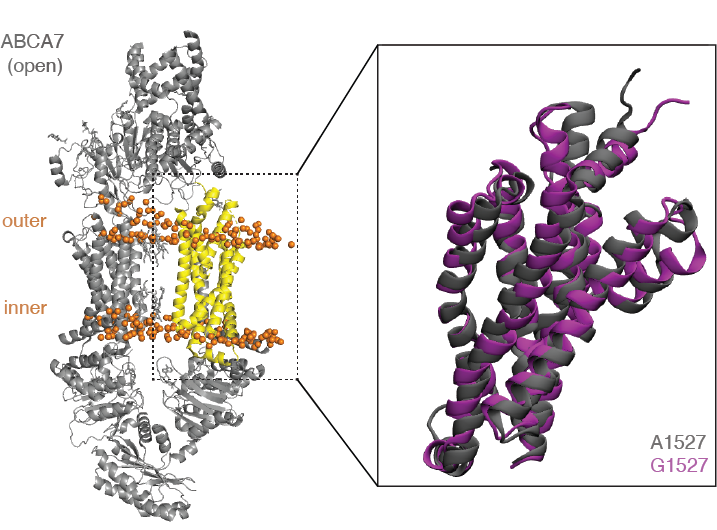
\includegraphics[width=\textwidth]{../paper/extended_plots/abca7_structure_with_inset.png}        
    \end{subfigure}
    %\hspace{1cm}
    \begin{subfigure}[t]{.25\textwidth}
        \caption{}
        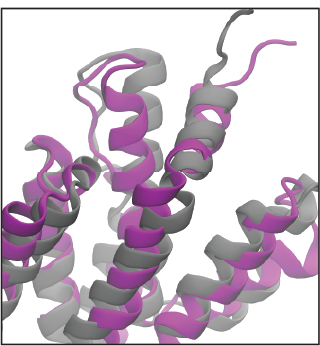
\includegraphics[width=\textwidth]{../paper/extended_plots/abca7_structure_inset_only.png}        
    \end{subfigure}
    \begin{subfigure}[t]{.33\textwidth}
        \caption{}
        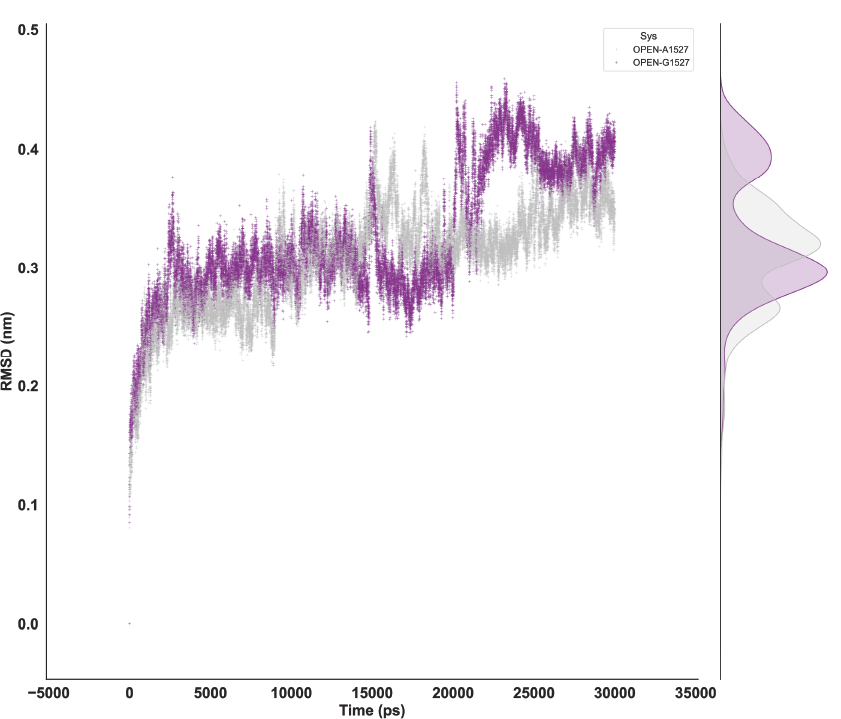
\includegraphics[width=\textwidth]{../paper/extended_plots/rmsd_time.png}        
    \end{subfigure}
    \hspace{1cm}
    \begin{subfigure}[t]{.25\textwidth}
        \caption{}
        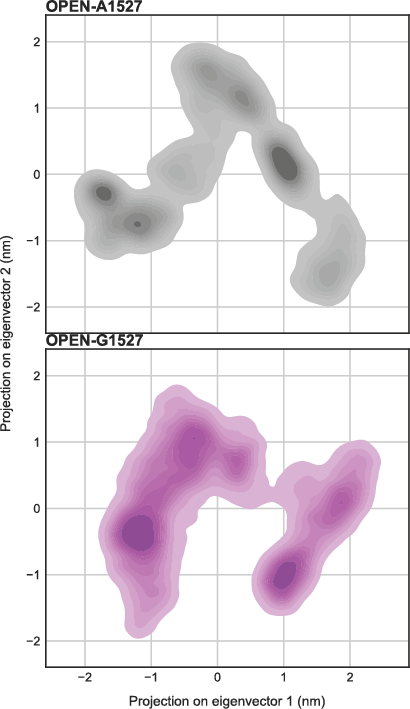
\includegraphics[width=\textwidth]{../paper/extended_plots/rmsd_projection_open.png}        
    \end{subfigure}
    \hspace{1cm}
    \begin{subfigure}[t]{.5\textwidth}
        \caption{}
        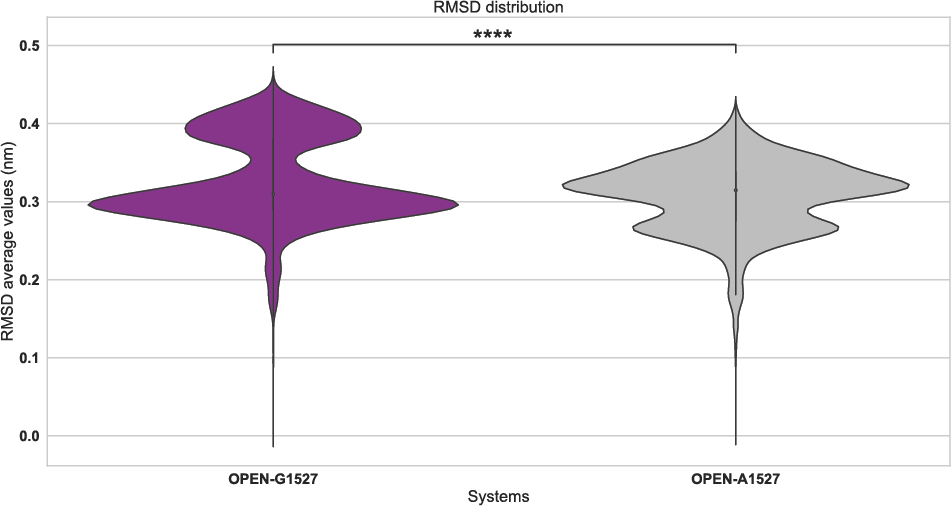
\includegraphics[width=\textwidth]{../paper/extended_plots/rmsd_volcano.png}        
    \end{subfigure}
\end{figure}
\textbf{Extended Data Fig. 6}
\clearpage
% Differentiating iPSC neurons
\begin{figure}[H]
    \begin{subfigure}[t]{0.3\textwidth}
        \begin{subfigure}[t]{\textwidth}
            \caption{}
            \includegraphics[width=\textwidth]{./extended_plots/glu50fs3_cartoon.png}        
        \end{subfigure}    
        \begin{subfigure}[t]{\textwidth}
            \caption{}
            \includegraphics[width=\textwidth]{./extended_plots/tyr622_cartoon.png}        
        \end{subfigure}  
    \end{subfigure}  
    \begin{subfigure}[t]{0.2\textwidth}
        \caption{}
        \includegraphics[width=\textwidth]{./extended_plots/karyotypes.png}        
    \end{subfigure}  
    \begin{subfigure}[t]{0.4\textwidth}
        \begin{subfigure}[t]{\textwidth}
            \caption{}
            \includegraphics[width=\textwidth]{./extended_plots/iN_induction_cartoon.png}        
        \end{subfigure}    
        \begin{subfigure}[t]{\textwidth}
            \caption{}
            \includegraphics[width=\textwidth]{./extended_plots/iN_markers.png}        
        \end{subfigure}  
    \end{subfigure}    
    \caption{
        \textbf{Differentiating and Profiling iPSC-Derived Neurons Harboring ABCA7 PTC Variants.}\\
    }
    \label{fig:differentiating_iPSC_neurons}
\end{figure}
\begin{itemize}
    \item[\textbf{(A)}] Sanger sequencing chromatogram confirming single nucleotide insertion in ABCA7 exon 3 to introduce a premature termination codon into the isogenic iPSC line ABCA7 p.Glu50fs*3 using CRISPR-Cas9 gene editing. 
    \item[\textbf{(B)}] Sanger sequencing chromatogram confirming patient single nucleotide polymorphism in ABCA7 exon 15 to introduce a premature termination codon into the isogenic iPSC line ABCA7 p.Tyr622* using CRISPR-Cas9 gene editing. 
    \item[\textbf{(C)}] Normal karyotypes were observed for control, ABCA7 p.Glu50fs*3, and ABCA7 p.Tyr622* isogenic iPSC lines. 
    \item[\textbf{(D)}] iPSCs were plated at low density for NGN2 viral transduction. Expression of NGN2 was driven by doxycycline (DOX) induction with puromycin (PURO) selection, then re-plated to match neuronal densities. Neurons were maintained for 4 weeks (DIV 28) before experimentation (Created with BioRender.com). 
    \item[\textbf{(E)}] Neuronal marker gene expression in 2 and 4-week matured iNs. 
\end{itemize}
\clearpage
% bulk RNAseq supplement
\begin{figure}[ht]
    \begin{subfigure}[t]{.3\textwidth}
        \caption{}
        \includegraphics[width=\textwidth]{./extended_plots/jaccard_pT622_pG50fs3_vs_wt.png}        
    \end{subfigure}
    \begin{subfigure}[t]{.3\textwidth}
        \caption{}
        \includegraphics[width=\textwidth]{./extended_plots/rna_correlation_miocarta_both_lines.png}        
    \end{subfigure}
    \begin{subfigure}[t]{.3\textwidth}
        \caption{}
        \includegraphics[width=\textwidth]{./extended_plots/correlation_with_other_RNAseq_batch.png}        
    \end{subfigure}
    \caption{
        \textbf{Bulk RNAseq data in iN.}\\[1ex]
        (A) Lipid synthesis and storage pathways perturbed in ABCA7 LoF excitatory neurons vs. control as measured by snRNA-seq on the post-mortem human PFC. Enrichments of biological processes were computed using FGSEA. Red = enrichment > 0, Blue = enrichment < 0. * = $p<0.05$. 
        (B) Schematic model showing anabolic processes feeding from the TCA cycle towards fatty acid (FA) and triglyceride (TG) synthesis. DG = diacylglyceride, PA = phosphatidic acid, PC = phosphatidylcholine, PE = phosphatidylethanolamine, PS = phosphatidylserine. * = differentially expressed in ABCA7 LoF vs. control excitatory neurons from post-mortem human brain at $p<0.05$ and $\log\text{FC}<0$. 
        (C) 𝛽-oxidation and TCA pathways perturbed in ABCA7 LoF excitatory neurons vs. control as measured by snRNA-seq on the post-mortem human PFC. Enrichments of biological processes were computed using FGSEA. Red = enrichment > 0, Blue = enrichment < 0. * = $p<0.05$. 
        (D) Schematic model showing catabolic processes feeding into the TCA cycle and oxidative phosphorylation with key genes from (C) highlighted in red or blue. * = $p<0.05$. For (A, C,) boxes indicate per-condition dataset quartiles, and whiskers extend to the most extreme data points not considered outliers (i.e., within 1.5 times the interquartile range from the first or third quartile). 
        (E, F) Transcript levels of ACLY (E) and SCP2 (F) assessed in post-mortem human PFC by RNAscope. Transcript counts per SLC17A7+ cell are reported in each bar chart. $N = 8$ individuals per genotype. Per-cell Wilcoxon rank-sum p-values are reported.
    }
    \label{fig:bulk_RNAseq_supplement}
\end{figure}
\clearpage
% LCMS supplement
\begin{figure}[ht]
    \begin{subfigure}[t]{0.5\textwidth}
        \caption{}
        \includegraphics[width=\textwidth]{./extended_plots/lcms_corr_heatmap.png}        
    \end{subfigure}  
    \begin{subfigure}[t]{0.5\textwidth}
        \caption{}
        \includegraphics[width=\textwidth]{./extended_plots/lcms_corr_scatterplot.png}        
    \end{subfigure}  
    \begin{subfigure}[t]{0.5\textwidth}
        \caption{}
        \includegraphics[width=\textwidth]{./extended_plots/lcms_corr_scatterplot_metab.png}        
    \end{subfigure}  
    \begin{subfigure}[t]{0.5\textwidth}
        \caption{}
        \includegraphics[width=\textwidth]{./extended_plots/beta_ox_genes_pm.png}        
    \end{subfigure}  
    \caption{
        \textbf{LCMS supplement in iN.}\\[1ex]
        (A) Lipid synthesis and storage pathways perturbed in ABCA7 LoF excitatory neurons vs. control as measured by snRNA-seq on the post-mortem human PFC. Enrichments of biological processes were computed using FGSEA. Red = enrichment > 0, Blue = enrichment < 0. * = $p<0.05$. 
        (B) Schematic model showing anabolic processes feeding from the TCA cycle towards fatty acid (FA) and triglyceride (TG) synthesis. DG = diacylglyceride, PA = phosphatidic acid, PC = phosphatidylcholine, PE = phosphatidylethanolamine, PS = phosphatidylserine. * = differentially expressed in ABCA7 LoF vs. control excitatory neurons from post-mortem human brain at $p<0.05$ and $\log\text{FC}<0$. 
        (C) 𝛽-oxidation and TCA pathways perturbed in ABCA7 LoF excitatory neurons vs. control as measured by snRNA-seq on the post-mortem human PFC. Enrichments of biological processes were computed using FGSEA. Red = enrichment > 0, Blue = enrichment < 0. * = $p<0.05$. 
        (D) Schematic model showing catabolic processes feeding into the TCA cycle and oxidative phosphorylation with key genes from (C) highlighted in red or blue. * = $p<0.05$. For (A, C,) boxes indicate per-condition dataset quartiles, and whiskers extend to the most extreme data points not considered outliers (i.e., within 1.5 times the interquartile range from the first or third quartile). 
        (E, F) Transcript levels of ACLY (E) and SCP2 (F) assessed in post-mortem human PFC by RNAscope. Transcript counts per SLC17A7+ cell are reported in each bar chart. $N = 8$ individuals per genotype. Per-cell Wilcoxon rank-sum p-values are reported.
    }
    \label{fig:lipid_mitochondrial_perturbations}
\end{figure}

\clearpage
% mitochondrial o2 consumption
\begin{figure}[H]
    \begin{subfigure}[t]{0.33\textwidth}
        \caption{}
        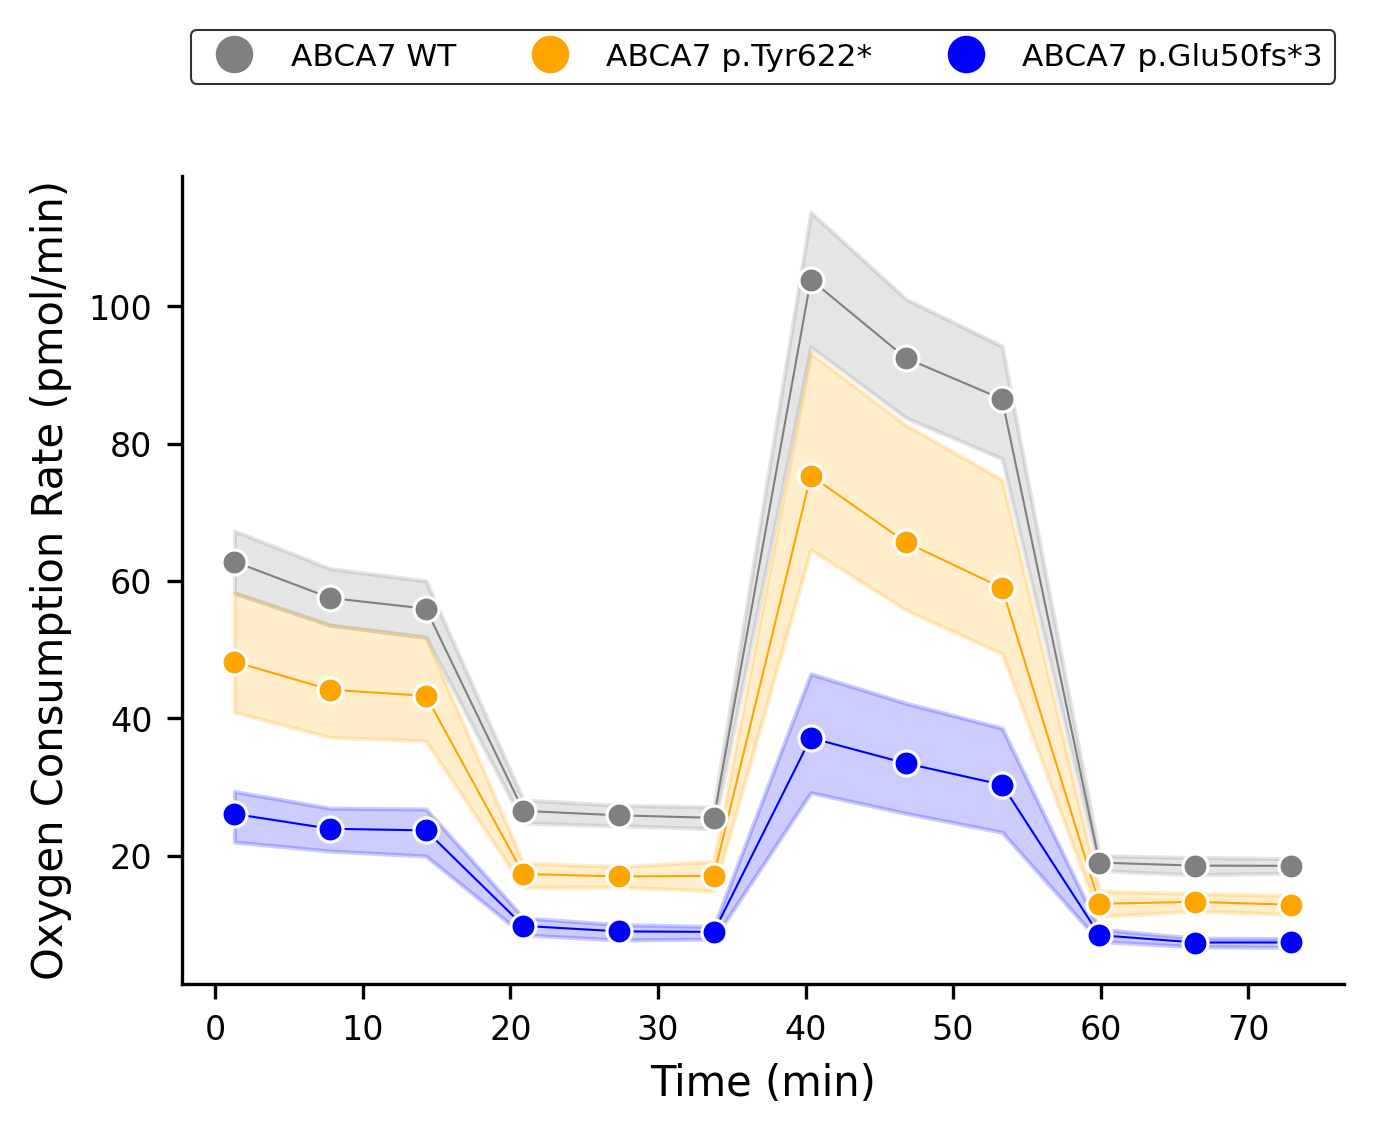
\includegraphics[width=\textwidth]{../paper/extended_plots/rep_seahorse_curves_by_line.png}        
    \end{subfigure}
    \begin{subfigure}[t]{0.33\textwidth}
        \caption{}
        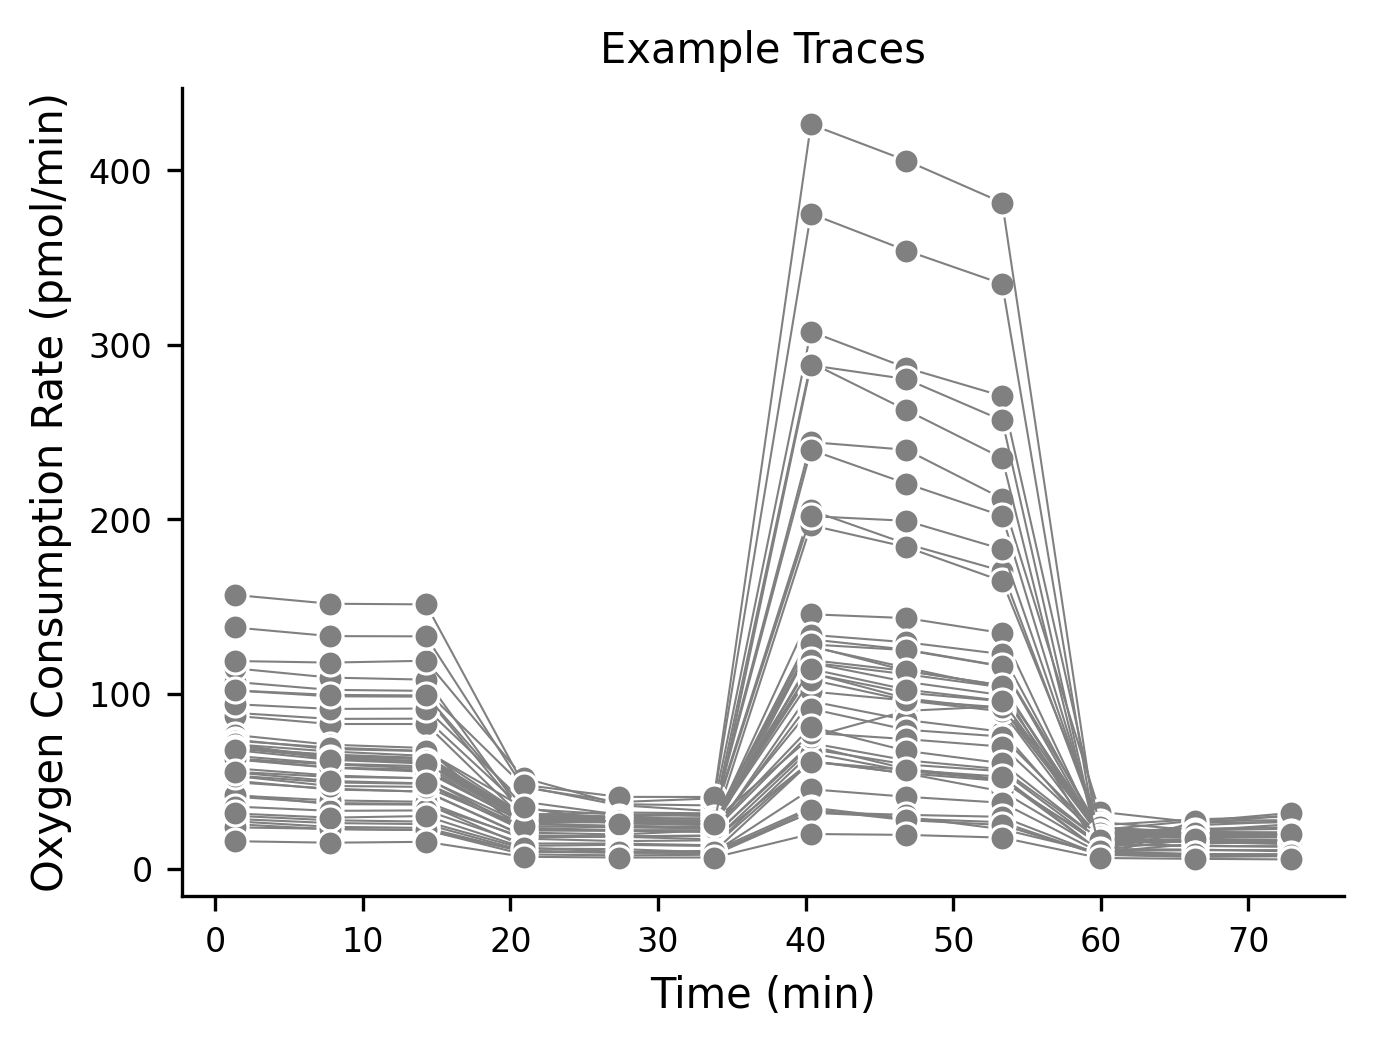
\includegraphics[width=\textwidth]{../paper/extended_plots/rep_seahorse_curves_all.png}        
    \end{subfigure}   
    \begin{subfigure}[t]{0.33\textwidth}
        \caption{}
        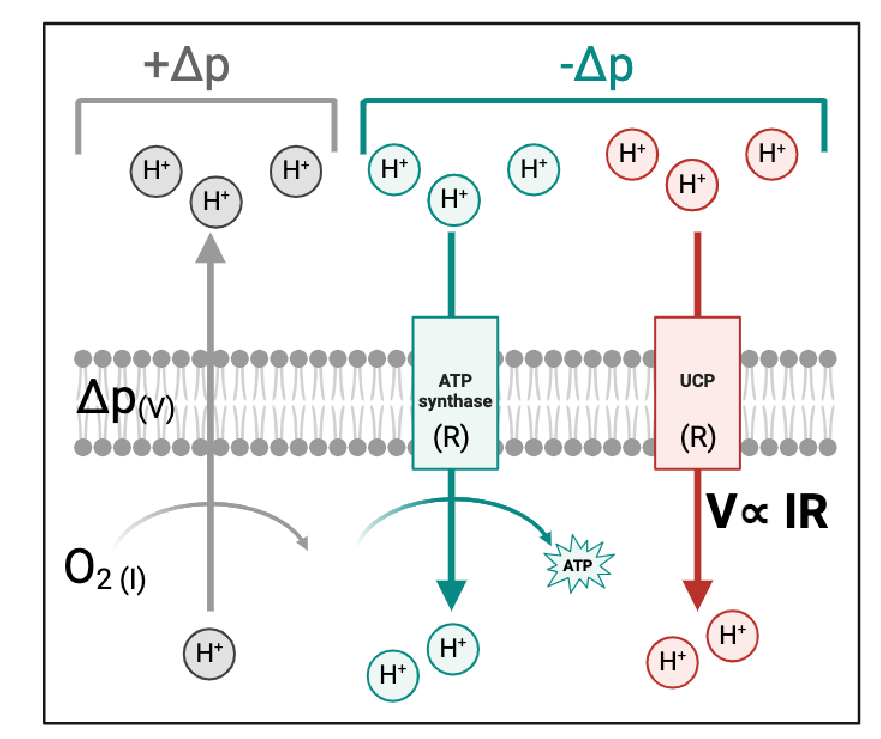
\includegraphics[width=\textwidth]{../paper/main_plots/uncoupling_cartoon.png}        
    \end{subfigure}  
    \begin{subfigure}[t]{0.33\textwidth}
        \caption{}
        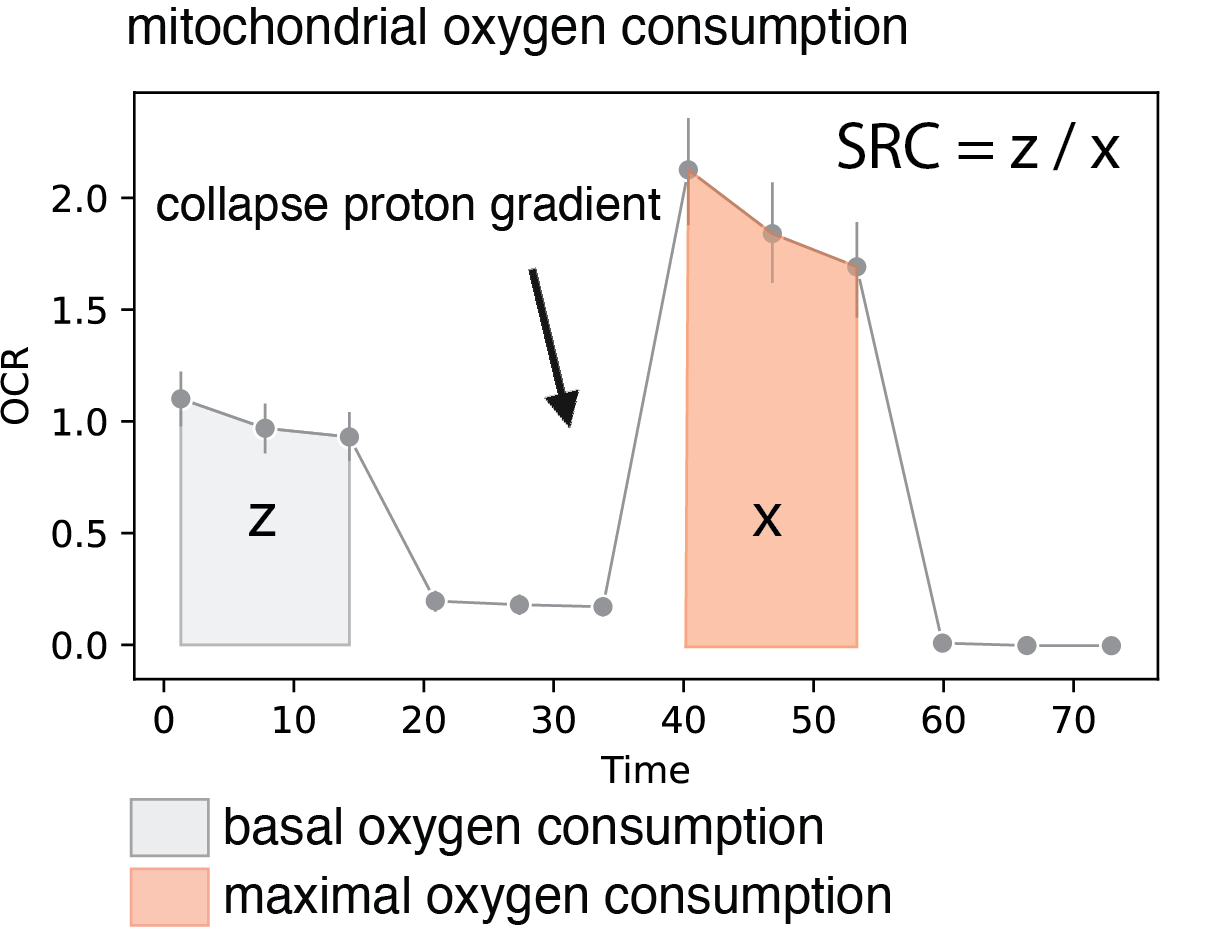
\includegraphics[width=\textwidth]{../paper/extended_plots/src_cartoon.png}        
    \end{subfigure} 
    \begin{subfigure}[t]{0.25\textwidth}
        \caption{}
        \includegraphics[width=\textwidth]{../paper/extended_plots/SRC.png}        
    \end{subfigure} 
    \begin{subfigure}[t]{0.33\textwidth}
        \caption{}
        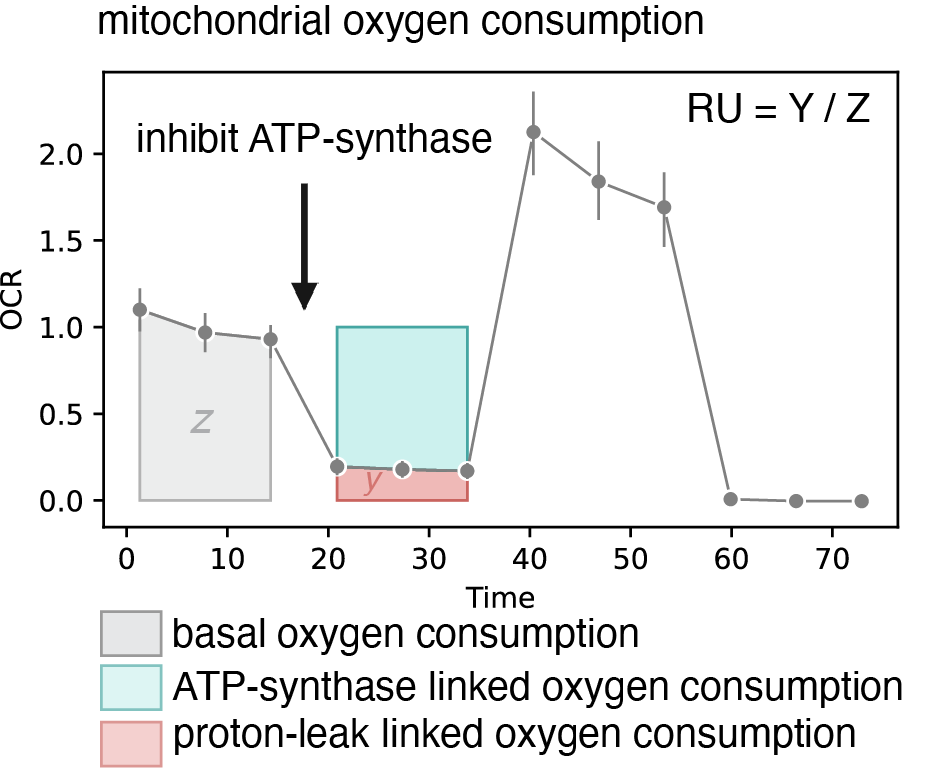
\includegraphics[width=\textwidth]{../paper/main_plots/seahorse_cartoon.png}        
    \end{subfigure}  
    \hspace{1cm}
    \begin{subfigure}[t]{0.3\textwidth}
        \caption{}
        \includegraphics[width=\textwidth]{../paper/extended_plots/UCP_levels.png}        
    \end{subfigure} 
    \par
    \centering
    \begin{subfigure}[t]{0.65\textwidth}
        \caption{}
        \includegraphics[width=\textwidth]{../paper/main_plots/tmrm_with_FCCP.png}        
    \end{subfigure} 
 \end{figure}
\textbf{Extended Data Fig. 10}
\clearpage
% mitochondrial mmp
% \begin{figure}[ht]
    \begin{subfigure}[t]{0.7\textwidth}
        \caption{}
        \includegraphics[width=\textwidth]{./extended_plots/mitohealth_dye.png}        
    \end{subfigure}
    \par
    \begin{subfigure}[t]{\textwidth}
        \caption{}
        \includegraphics[width=\textwidth]{./extended_plots/mitohealth_per_cell.png}        
    \end{subfigure}
    \caption{
         \textbf{Analysis of Oxygen Consumption Rates in ABCA7 LoF vs. Control iNs.}\\[1ex]
         (A) Example oxygen consumption rate (OCR) curves from Batch 1 of the two differentiation batches used for analysis in Figure~\ref{fig:main_mitochondrial}G. The line plot indicates the per-condition mean estimator, and the error bars indicate the 95\% confidence interval. 
         (B) Representative per-well traces from (A). 
         (C) Schematic indicating measurement of maximal and basal oxygen consumption to compute SRC, as shown in 
         (D) for WT, ABCA7 p.Glu50fs*3, and ABCA7 p.Tyr622* iNs. P-values computed by independent sample t-test. $N$ wells = 18 (WT), 17 (p.Tyr622*), 13 (p.Glu50fs*3) across two independent differentiation batches and Seahorse experiments. 
         (E) Relative uncoupling measured for two independent iN differentiation batches and separate Seahorse experiments shown combined in Figure~\ref{fig:main_mitochondrial}G. P-values computed by independent sample t-test. Batch 1 (left); $N$ wells = 10 (WT), 7 (p.Tyr622*), 7 (p.Glu50fs*3). Batch 2 (right); $N$ wells = 8 (WT), 10 (p.Tyr622*), 6 (p.Glu50fs*3) shown per differentiation batch. For (D, E) boxes indicate per-condition dataset quartiles, and whiskers extend to the most extreme data points not considered outliers (i.e., within 1.5 times the interquartile range from the first or third quartile). 
         (F) Per-batch cell-level MioHealth fluorescence intensities (related to Figure~\ref{fig:main_mitochondrial}H).
     }
     \label{fig:oxygen_consumption_rates_iPSC_neurons}
 \end{figure}
% \clearpage
% choline treatment
\begin{figure}[ht]
    %ROW 1
    \begin{subfigure}[t]{.6\textwidth}
        \caption{}
        \includegraphics[width=\textwidth]{./extended_plots/choline_media_lcms.png}        
    \end{subfigure}
    \begin{subfigure}[t]{.35\textwidth}
        \caption{}
        \includegraphics[width=\textwidth]{./extended_plots/choline_in_cells_lcms.png}        
    \end{subfigure}
    %ROW 2
    \begin{subfigure}[t]{.25\textwidth}
        \caption{}
        \includegraphics[width=\textwidth]{./extended_plots/choline_synth_genes.png}        
    \end{subfigure}
    \begin{subfigure}[t]{.35\textwidth}
        \caption{}
        \includegraphics[width=\textwidth]{./main_plots/pc_unsat_with_choline_batch1.png}        
    \end{subfigure} 
    \begin{subfigure}[t]{0.25\textwidth}
        \caption{}
        \includegraphics[width=\textwidth]{./main_plots/rna_correlation_plot.png}        
    \end{subfigure}  
    \begin{subfigure}[t]{.2\textwidth}
        \caption{}
        \includegraphics[width=\textwidth]{./extended_plots/rna_correlation_miocarta_choline.png}        
    \end{subfigure}
    \begin{subfigure}[t]{.25\textwidth}
        \caption{}
        \includegraphics[width=\textwidth]{./extended_plots/ocr_choline_curves_by_treatment.png}        
    \end{subfigure}
    \begin{subfigure}[t]{.25\textwidth}
        \caption{}
        \includegraphics[width=\textwidth]{./extended_plots/ocr_choline_rep_curves.png}        
    \end{subfigure}
    \begin{subfigure}[t]{.2\textwidth}
        \caption{}
        \includegraphics[width=\textwidth]{./extended_plots/src_choline_quantification.png}        
    \end{subfigure}
    \begin{subfigure}[t]{.2\textwidth}
        \caption{}
        \includegraphics[width=\textwidth]{./extended_plots/mitohealth_choline.png}        
    \end{subfigure}
    \caption{
         \textbf{CDP-choline treatment in iN.}\\[1ex]
         (A) Per-cell correlation of average PLIN2 and LipidSpot fluorescent intensities shown as a density plot. 
         (B) Per-batch LipidSpot fluorescence intensities (related to Figure~\ref{fig:main_choline}A) in ABCA7 p.Tyr622* iNs treated with CDP-choline or H20 vehicle control. X-axis indicates z-scaled log-fluorescence intensity. 
         (C) Example oxygen consumption rate (OCR) curves used for analysis in Figure~\ref{fig:main_choline}. The line plot indicates the per-condition mean estimator, and the error bars indicate the 95\% confidence interval. 
         (D) Representative per-well traces from (C). 
         (E) Quantification of SRC from curves in (D). P-values computed by independent sample t-test. $N$ wells = 6 (p.Tyr622* + H20), 8 (p.Tyr622* + CDP-choline). Boxes indicate per-condition dataset quartiles, and whiskers extend to the most extreme data points not considered outliers (i.e., within 1.5 times the interquartile range from the first or third quartile). 
         (F) Per-batch cell-level MioHealth fluorescence intensities (related to Figure~\ref{fig:main_choline}C) in ABCA7 p.Tyr622* iNs treated with CDP-choline or H20 vehicle control. X-axis indicates z-scaled fluorescence intensity.
     }
     \label{fig:lipid_mitochondrial_effects_CDP_choline}
 \end{figure}

 

    % \begin{subfigure}[t]{.3\textwidth}
    %     \caption{}
    %     \includegraphics[width=\textwidth]{./main_plots/volcano_all_species_choline.png}        
    % \end{subfigure}
    % \begin{subfigure}[t]{.2\textwidth}
    %     \caption{}
    %     \includegraphics[width=\textwidth]{./extended_plots/desaturase_genes.png}        
    % \end{subfigure}
    % \begin{subfigure}[t]{.2\textwidth}
    %     \caption{}
    %     \includegraphics[width=\textwidth]{./extended_plots/desaturase_genes_e3_v_y622.png}        
    % \end{subfigure}
    % \par
\clearpage
% neurospheroid figure
\begin{figure}[ht]
    \begin{subfigure}[t]{\textwidth}
        \caption{}
        \includegraphics[width=\textwidth]{./extended_plots/neurospheroid_markers.png}        
    \end{subfigure}
    \begin{subfigure}[t]{0.2\textwidth}
        \caption{}
        \includegraphics[width=\textwidth]{./extended_plots/additional_abeta_timepoints.png}        
    \end{subfigure}
    \begin{subfigure}[t]{0.2\textwidth}
        \caption{}
        \includegraphics[width=\textwidth]{./extended_plots/other_choline_conc.png}        
    \end{subfigure}
    \begin{subfigure}[t]{0.2\textwidth}
        \caption{}
        \includegraphics[width=\textwidth]{./extended_plots/ephys_additional.png}        
    \end{subfigure}
    \begin{subfigure}[t]{0.2\textwidth}
        \caption{}
        \includegraphics[width=\textwidth]{./extended_plots/calcium_imaging.png}        
    \end{subfigure}
    \caption{
        \textbf{CDP-choline treatment in neurospheroids}\\[1ex]
        (A) Per cell type ABCA7 detection rate of major cell types in the post-mortem PFC as quantified by snRNA-seq. 
        (B) Normalized expression of indicated gene in glial cells (per-individual mean expression profiles across Oli, Opc, Ast, Mic) vs. neuronal cells (per-individual mean expression profiles across Ex and In) from post-mortem snRNA-seq data. 
        (C) Normalized expression of indicated genes in NeuN- vs. NeuN+ cells (N=6 individuals, from \cite{Welch2022-aa}; see Table 2). All p-values are computed by paired two-sided t-test. Boxes indicate per-condition dataset quartiles, and whiskers extend to the most extreme data points not considered outliers (i.e., within 1.5 times the interquartile range from the first or third quartile).
    }
    \label{fig:neurospheroid_figure}
\end{figure}

\clearpage
% updated model
\begin{figure}[ht]
    %\centerline{\includegraphics[width=\textwidth]{./extended_plots/lipid_mitochondrial_perturbations.pdf}}
    \caption{
        \textbf{Model of ABCA7 LoF dysfunction in neurons.}\\[1ex]
        (A) Lipid synthesis and storage pathways perturbed in ABCA7 LoF excitatory neurons vs. control as measured by snRNA-seq on the post-mortem human PFC. Enrichments of biological processes were computed using FGSEA. Red = enrichment > 0, Blue = enrichment < 0. * = $p<0.05$. 
        (B) Schematic model showing anabolic processes feeding from the TCA cycle towards fatty acid (FA) and triglyceride (TG) synthesis. DG = diacylglyceride, PA = phosphatidic acid, PC = phosphatidylcholine, PE = phosphatidylethanolamine, PS = phosphatidylserine. * = differentially expressed in ABCA7 LoF vs. control excitatory neurons from post-mortem human brain at $p<0.05$ and $\log\text{FC}<0$. 
        (C) 𝛽-oxidation and TCA pathways perturbed in ABCA7 LoF excitatory neurons vs. control as measured by snRNA-seq on the post-mortem human PFC. Enrichments of biological processes were computed using FGSEA. Red = enrichment > 0, Blue = enrichment < 0. * = $p<0.05$. 
        (D) Schematic model showing catabolic processes feeding into the TCA cycle and oxidative phosphorylation with key genes from (C) highlighted in red or blue. * = $p<0.05$. For (A, C,) boxes indicate per-condition dataset quartiles, and whiskers extend to the most extreme data points not considered outliers (i.e., within 1.5 times the interquartile range from the first or third quartile). 
        (E, F) Transcript levels of ACLY (E) and SCP2 (F) assessed in post-mortem human PFC by RNAscope. Transcript counts per SLC17A7+ cell are reported in each bar chart. $N = 8$ individuals per genotype. Per-cell Wilcoxon rank-sum p-values are reported.
    }
    \label{fig:lipid_mitochondrial_perturbations}
\end{figure}
\clearpage




% \begin{figure}[ht]
%    % \centerline{\includegraphics[width=\textwidth]{./extended_plots/quantification_Abeta42_iPSC_neurons.pdf}}
%     \caption{
%         \textbf{Quantification of Aβ42 in iPSC-Derived Neurons Harboring ABCA7 PTC Variants.}\\[1ex]
%         (A) Quantification of neuronal Aβ42 fluorescence intensity. P-values were computed by a linear mixed-effects model on per-NeuN+ volume averages, including well-of-origin as a random effect. $N = 16$ (WT; 2261 cells), $N=8$ (p.Tyr622*; 1466 cells), $N=6$ wells (p.Glu50fs*3; 999 cells) from 4-week-old iNs. Boxes indicate per-condition dataset quartiles, and whiskers extend to the most extreme data points not considered outliers (i.e., within 1.5 times the interquartile range from the first or third quartile). Individual data points represent per-well averages of cell-level intensities. 
%         (B) Representative images per condition showing mean-intensity projections of the entire image (NeuN+) and projections within NeuN+ volumes considered for quantification (Aβ42). Representative images for the Aβ42 channel were processed with condition-wide percentile-based background subtraction and thresholding. Representative images of cell soma underwent per-image percentile-based background subtraction and thresholding, reflecting the segmentation methodology.
%     }
%     \label{fig:quantification_Abeta42_iPSC_neurons}
% \end{figure}



  \clearpage
  \subsubsection*{Supplementary Notes}
\phantomsection
\addcontentsline{toc}{subsubsection}{Supplementary Notes}

\paragraph*{Supplementary Note 1.}
\phantomsection
\addcontentsline{toc}{paragraph}{Supplementary Note 1.}
Description of variables according to the Rush Alzheimer’s Disease Center Codebook.
\begin{enumerate}
    \item \textbf{study}: Indicates the cohort participants were recruited through: Religious Orders Study (ROS) or Memory and Aging Project (MAP)\supercite{Bennett2018-tn}.
    
    \item \textbf{pmi}: Postmortem interval, defined as the number of hours from the participant’s time of death until autopsy and tissue preservation.
    
    \item \textbf{age\_death}: Participant's age at the time of death.
    
    \item \textbf{msex}: Participant's self-reported sex, coded as “1” for male and “0” for female.
    
    \item \textbf{amyloid}: Mean amyloid-beta load, quantified as the percent cortical area occupied by amyloid-beta deposits via immunohistochemistry, averaged across 8 brain regions (at least 4 required): hippocampus, entorhinal cortex, midfrontal cortex, inferior temporal gyrus, angular gyrus, calcarine cortex, anterior cingulate cortex, and superior frontal cortex.
    
    \item \textbf{ceradsc}: CERAD neuropathological score providing a semiquantitative measure of neuritic plaque density, categorized into definite AD (1), probable AD (2), possible AD (3), or no AD (4), determined independently of age or clinical data.
    
    \item \textbf{nft}: Summary measure of neurofibrillary tangle burden, derived by microscopic assessment of silver-stained slides from five brain regions (midfrontal cortex, midtemporal cortex, inferior parietal cortex, entorhinal cortex, hippocampus), standardized regionally, and averaged into a single value.
    
    \item \textbf{braaksc}: Semi-quantitative Braak stage score for severity and distribution of neurofibrillary tangles (NFTs), assessed with Bielschowsky silver stain in the frontal, temporal, parietal, entorhinal cortex, and hippocampus: stages I-II indicate tangles primarily in entorhinal regions; stages III-IV signify limbic involvement such as hippocampus; and stages V-VI show moderate to severe neocortical involvement.
    
    \item \textbf{cogdx}: Final clinical consensus diagnosis regarding cognitive status at the time of death, derived by expert neurologists reviewing all available clinical data without knowledge of postmortem findings. Categories include: no cognitive impairment (1), mild cognitive impairment without other causes (2), mild cognitive impairment with another cause (3), Alzheimer's disease without another cause (probable AD) (4), Alzheimer's disease with another cause (possible AD) (5), and other primary dementia (6).
    
    \item \textbf{niareagansc}: The NIA-Reagan neuropathological scoring system classifies Alzheimer's disease likelihood into four levels (1: high, 2: intermediate, 3: low, 4: no AD) based on combined assessment of neurofibrillary tangles (Braak) and neuritic plaques (CERAD), evaluated postmortem without knowledge of clinical dementia status.
    
    \item \textbf{ad\_reagan}: Dichotomized version of the NIA-Reagan neuropathological score, categorizing participants into Alzheimer's-positive (1: high/intermediate) or Alzheimer's-negative (0: low/no AD).
    
    \item \textbf{apoe\_genotype}: APOE genotype identified by DNA extraction from peripheral blood mononuclear cells or brain tissue, using high-throughput sequencing to genotype codon 112 and codon 158 in exon 4 of the APOE gene on chromosome 19.
\end{enumerate}
  \clearpage
  \subsubsection*{Supplementary Note 2}
\addcontentsline{toc}{subsubsection}{Supplementary Note 2: Choosing a partitioning heuristic for gene-pathway grouping}
\textbf{Choosing a partitioning heuristic for gene-pathway grouping}
\paragraph{Methods.}
The heatmap in Supplementary Figure 3a highlights how frequently pathways within a pathway database, such as WikiPathways, share gene members. On average, every pathway shown in Supplementary Figure 3a shares at least one gene with approximately 40\% of the other pathways, highlighting that there is redundancy in this matrix that could be summarized in simpler terms.

To summarize redundant gene-pathway information into a limited number of non-redundant gene-pathway groups, we reformulated the gene-pathway association problem as a bipartite graph $G$ constructed from all the genes in the Leading Edge subset (LE) and their associated pathways. LE was defined as the set of 268 genes driving the enrichment signal for pathways that passed a significance threshold of $p < 0.05$ (fGSEA) in Con vs. ABCA7 LoF excitatory neurons. $G$ was constructed from an $n \times m$ unweighted adjacency matrix, where $n$ represented the number of LE genes and $m$ the number of pathways associated with four or more LE genes, as specified in the WikiPathways database.

Graph partitioning involves segmenting the vertices of a graph into equal-sized partitions, optimizing for the minimal number of interconnecting edges (i.e., “total cut size”). We tested three prominent graph partitioning techniques, as outlined by Elsner (1997) \supercite{Elsner1997GraphPartitioning}, to approximate optimal partitioning. These methods include:

\begin{enumerate}
    \item \textbf{Recursive Spectral Bisection}: Implemented in Python using the numpy linear algebra package, this method was executed for $\log_2(N)$ iterations, yielding $N = 8$ partitions. A detailed description of the algorithm can be found in Elsner (1997)\supercite{Elsner1997GraphPartitioning}.
    \item \textbf{Multilevel Graph Partitioning}: Leveraging the METIS software package \supercite{Karypis1997METIS} in Python using the following parameters: `nparts=8`, `tpwgts=None`, `ubvec=None`, `recursive=False`.
    \item \textbf{Kernighan-Lin (K/L) Algorithm}: Based on its original paper\supercite{Kernighan1970-zl}, this algorithm was implemented in Python and run with parameters set as $C=0$, `KL\_modified=True`, `random\_labels=True`, `unweighted=True`, and $K=50$.
\end{enumerate}

Additionally, the Spectral Clustering algorithm, a commonly used clustering method, was applied using the `SpectralClustering()` function from the `sklearn` Python package with default parameters, apart from `n\_clusters=8` and `assign\_labels='kmeans'`. We stipulated eight clusters for each algorithm, as qualitatively, this resolution seemed to strike a good balance to summarize main biological effects.

For benchmarking purposes, the three graph partitioning techniques and the spectral clustering algorithm were evaluated by segmenting graph $G$ into eight gene-pathway clusters using the respective algorithms. Spectral clustering was run over 1,000 initiations, while K/L and METIS were run over 50,000 iterations because their solutions were slightly more variable across runs. The deterministic bisection method was run only once. A randomized graph partitioning benchmark was also computed by permuting the eight cluster labels of approximately equivalent size for 1,000 initiations. Average losses were computed per algorithm on all initiations. The benchmarking process and source code are available at: GitHub Repository.

\paragraph{Results.}
Spectral clustering performed significantly better than all other algorithms based on the loss (Supplementary Figure 3b). This was expected, as spectral clustering does not place a constraint on cluster size. Spectral clustering results were characterized by a single large cluster and many small clusters (Supplementary Figure 3c), indicating that this clustering algorithm was highly susceptible to outliers and suggesting that graph partitioning, which imposes the constraint of equal partitioning, was a better approach to the problem of grouping genes and pathways into biologically informative groups. Indeed, all three graph partitioning algorithms divided the graph into more uniformly-sized groups (Supplementary Figure 3c). Among the partitioning algorithms, K/L and METIS produced the most uniformly sized groups (Supplementary Figure 3c) and also had significantly lower losses compared to the spectral bisection algorithm (Supplementary Figure 3b). K/L and METIS solutions were very similar, with their respective best solutions (lowest loss) having an average Jaccard similarity index of 0.91 on the diagonal (Supplementary Figure 3d,e). K/L and METIS solutions were also consistent across pairwise random initiations, both when comparing within K/L or METIS solutions (Rand Index=0.87 and 0.91, respectively) and when comparing all pairwise K/L and METIS solutions (Rand Index=0.88) (Supplementary Figure 3f).

Overall, these results indicate the importance of non-redundant gene-pathway groupings to interpret biological effects. They also indicate that for some gene-pathway graphs, such as the one in this study, graph partitioning is a better approach than clustering.

  \clearpage
  \subsubsection{Molecular Dynamics Simulations Results} 
\paragraph{RMSD analysis of Ala1527 vs Gly1527 in open and closed states.}
To evaluate conformational stability, we conducted root mean square deviation (RMSD) analyses on ABCA7 under different states and mutations (Figure~\ref{fig:main_neurons}G,H; Figure~\ref{fig:md_simulations}A,B; Table~\ref{tab:abca7_structures}). RMSD values for the $C_\alpha$ atoms were calculated over the course of a 300 ns simulation period, comparing closed and open conformations, each harboring either the G1527 or A1527 mutation.

For the open ABCA7 conformation, both the G1527 and A1527 mutants exhibited relatively minor RMSD fluctuations (Figure~\ref{fig:md_simulations}A-D), with RMSD values for the A1527 mutant significantly lower compared to those of the G1527 mutant (Figure~\ref{fig:md_simulations}E). Overall, both mutants showed narrow RMSD distributions in the open state (Figure~\ref{fig:md_simulations}C, D), indicating generally stable conformational behavior. 

Differences in RMSD distributions between the two variants became more pronounced in the closed state: The RMSD profile of the closed conformation with the G1527 mutation exhibited substantial fluctuations throughout the simulation (Figure~\ref{fig:main_neurons}I), suggesting that the G1527 mutation significantly increases local structural flexibility. In contrast, the closed conformation harboring the A1527 mutation showed only minor RMSD fluctuations (Figure~\ref{fig:main_neurons}I), suggesting that the A1527 mutation confers greater structural stability and reduced flexibility in the closed ABCA7 conformation. Principal component analysis (PCA) further highlighted these differences visually; For the closed conformation, PCA projections of G1527 conformations over time were broad, indicating significant exploration of the conformational space (Figure~\ref{fig:main_neurons}J). Conversely, the PCA plot for the closed A1527 mutant displayed a tightly clustered distribution (Figure~\ref{fig:main_neurons}J), indicating limited conformational sampling over time and suggesting decreased conformational flexibility induced by the A1527 mutation.

\paragraph{Dihedral angle analysis of Ala1527 vs Gly1527 in open and closed states.}
\newcommand{\quoteM}{\textcolor{blue}{To further explore the local structural variations induced by a p.Ala1527Gly mutation, we analyzed backbone dihedral angles (phi/psi; $\phi/\psi$) for residues 1517-1537. In the open conformation, Gly1527 consistently occupied the $\alpha$-helical region of the Ramachandran plot throughout the simulation. In contrast, Ala1527 showed two distinct populations within the $\alpha$-helical region (Figure~\ref{fig:md_simulations_2}A), suggesting subtle local conformational differences, yet overall preservation of the $\alpha$-helical structure. These findings align closely with the RMSD analysis, and suggest similar conformational behaviors between the variants in the open state. \label{quoteM-label}}}

\quoteM

\newcommand{\quoteN}{\textcolor{blue}{However, significant structural differences emerged in the closed conformation: Ala1527 displayed two preferred conformations—one within the $\alpha$-helical region and another shifted toward the $\beta$-structure region—while Gly1527 explored a broader range of dihedral angles, indicative of greater structural flexibility (Figure~\ref{fig:md_simulations_2}A,B). This observation is in line with the RMSD analysis, indicating structural differences specifically in the closed state, with Gly1527 exhibiting significantly greater conformational flexibility compared to Ala1527.}}

\quoteN

\paragraph{Secondary structure analysis of Ala1527 vs Gly1527 in open and closed states.}
\newcommand{\quoteO}{\textcolor{blue}{To complement backbone angle analysis, we also evaluated secondary structure stability throughout the simulation. In the open state, secondary structure content was comparable between variants, maintaining similar $\alpha$-helical character (Figure~\ref{fig:md_simulations_2}C). Upon transitioning to the closed state, both variants experienced a substantial loss of $\alpha$-helical content across residues 1517-1537. This loss, however, was more pronounced in the Gly1527 variant compared to the Ala1527 variant, as residues 1520-1525 retained partial $\alpha$-helical structure more robustly in the Ala1527 variant compared to Gly1527 (Figure~\ref{fig:md_simulations_2}C).}}

\quoteO

Finally, structural alignment of the closed-state Gly1527 ABCA7 structure (PDB 8EOP) with the closed-state structures of ABCA1 (PDB 7TBW) and ABCA4 (PDB 7LKZ) revealed that residues corresponding to Gly1527 in ABCA7 (V1646 in ABCA1; I1671 in ABCA4) adopt stable $\alpha$-helical structures (Figure~\ref{fig:md_simulations_2}E,F). In contrast, the Gly1527 residue in ABCA7 exhibits significant flexibility and lacks defined $\alpha$-helical structure. Interestingly, our simulations indicate that the Ala1527 variant partially restores this local $\alpha$-helical conformation in ABCA7 (Figure~\ref{fig:md_simulations_2}C,D). These data suggest that the Gly1527 variant induces local structural changes that differentiate ABCA7 from its close homologs ABCA1 and ABCA4.

  \clearpage
  \captionsetup{justification=raggedright,singlelinecheck=false}

\clearpage
\begin{longtable}{p{3cm} p{3cm} p{3cm} p{2cm} p{2.5cm} p{0.5cm}}
    \caption{Annotation of ABCA7 loss of function variants used in this study.}
    \hline
    \textbf{rsID}          & \textbf{HGVS.c}           & \textbf{HGVS.p}    & \textbf{Annotation}                                                           & \textbf{AD association}                                                                   & \textbf{N in cohort} \\
    \hline
    \hline
    rs113809142            & c.4416+2T>G               & NA                 & splice donor variant \cite{Allen2017-ch}                                      & Steinberg et al (2015), Nature Genetics, Table 1 \cite{Steinberg2015-wy}                   & 1 \\
    \hline
    rs200538373            & c.5570+5G>C               & NA                 & splice region variant \cite{Allen2017-ch,Steinberg2015-wy}                    & Steinberg et al (2015), Nature Genetics, Table 1 \cite{Steinberg2015-wy}                   & 4 \\
    \hline
    rs538591288            & c.4208delT                & p.Leu1403fs        & frameshift variant \cite{Allen2017-ch}                                        & Steinberg et al (2015), Nature Genetics, Table 1 \cite{Steinberg2015-wy}                   & 1 \\
    \hline
    rs547447016            & c.2126\_2132delAGCAGGG    & p.Glu709fs         & frameshift variant \cite{Allen2017-ch}                                        & Steinberg et al (2015), Nature Genetics, Table 1 \cite{Steinberg2015-wy}                   & 4 \\
    \hline
    rs201060968            & c.3641G>A                & p.Trp1214*         & stop gained                                                                   & NA                                                                                        & 1 \\
    \hline
    19\_1053362\_G\_A       & c.3255G>A                & p.Trp1085*         & stop gained                                                                   & NA                                                                                        & 1 \\
    \hline
    \label{tab:annotation_abca7}
\end{longtable}

\clearpage
\begin{longtable}{p{6cm} p{9cm}}
    \caption{PCR/Sanger sequencing (SS) primers.}
    \hline
    \textbf{Primer} & \textbf{Sequence} \\
    \hline
    \hline
    rs547447016\_FOR              & 5’-ACGCTGGCCTGGATCTACTC-3’ \\
    \hline
    rs547447016\_REV              & 5’-TGCATGCGTGTGCCAAGAAG-3’ \\
    \hline
    chr19.1053362G>A\_rs201060968\_FOR   & 5’-CTGAAGCACCCCTTTGTCCAC-3’ \\
    \hline
    chr19.1053362G>A\_rs201060968\_REV   & 5’-GAAAGCGCTTGAGAAGCAGGG-3’ \\
    \hline
    chr19.1053362G>A\_REV\_SS      & 5’-GCTGCTCATAAACACGCTATTCATCCTTC-3’ \\
    \hline
    rs201060968\_FOR\_SS          & 5’-CATTGCTGGCCTAGACGTAA-3’ \\
    \hline
    ABCA7\_p.Glu50fs*3\_FOR       & 5’-GTGACGAAAGCGTTAAGCCC-3’ \\
    \hline
    ABCA7\_p.Glu50fs*3\_REV       & 5’-GCAGTGGCTTGTTTGGGAAG-3’ \\
    \hline
    ABCA7\_p.Tyr622*\_FOR         & 5’-CTGGTTCTGGTGCTCAAG-3’ \\
    \hline
    ABCA7\_p.Tyr622*\_REV         & 5’-CCTACGGCAGACGTCTTCAG-3’ \\
    \label{tab:pcr_primers}
\end{longtable}

\clearpage
\begin{longtable}{p{5cm} p{5cm} p{5cm}}
    \caption{Experimentally-determined 3D ABCA7 structures used in molecular dynamics simulations.}
    \hline
    \textbf{System}    & \textbf{PDB ID} & \textbf{State} \\
    \hline
    \hline
    CLOSE-G1527        & 8EOP           & HOLO         \\
    \hline
    CLOSE-A1527        & 8EOP           & HOLO         \\
    \hline
    OPEN-G1527         & 8EE6           & APO          \\
    \hline
    OPEN-A1527         & 8EE6           & APO          \\
    \hline
    \label{tab:abca7_structures}
\end{longtable}

% \begin{table}[ht]
%     \centering
    %\resizebox{\textwidth}{!}{
\clearpage
\begin{longtable}{p{1.5cm} p{4cm} p{5cm} p{1.5cm} p{1.5cm} p{1.5cm}}
    \caption{Cluster 2 genes for p.Tyr622* vs WT bulk RNA-seq}
    \hline
    \textbf{Gene} & \textbf{Name} & \textbf{Function} & \textbf{logFC} & \textbf{P.Value} & \textbf{adj.P.Val} \\
    \hline
    \hline
    MVD    & Mevalonate Diphosphate Decarboxylase      & Catalyzes a key decarboxylation step in the mevalonate pathway for cholesterol and isoprenoid synthesis. & -0.806566 & $6.153354\times10^{-7}$ & 0.000101 \\
    \hline
    SQLE   & Squalene Epoxidase                       & Converts squalene to oxidosqualene in cholesterol biosynthesis.  & -0.658307 & $2.820266\times10^{-6}$ & 0.000311 \\
    \hline
    MSMO1  & Methylsterol Monooxygenase 1             & Involved in cholesterol biosynthesis; catalyzes conversion of methylsterols. & -0.559031 & $2.906982\times10^{-5}$ & 0.001650 \\
    \hline
    LSS    & Lanosterol Synthase                      & Catalyzes conversion of oxidosqualene to lanosterol in cholesterol synthesis.  & -0.931772 & $3.693352\times10^{-5}$ & 0.001908 \\
    \hline
    SC5D   & Sterol-C5-Desaturase                     & Catalyzes a desaturation step in the cholesterol biosynthetic pathway. & -0.478859 & $4.171666\times10^{-5}$ & 0.002105 \\
    \hline
    LDLR   & Low-Density Lipoprotein Receptor         & Mediates the uptake of cholesterol-rich LDL particles.  & -0.844660 & $4.693678\times10^{-5}$ & 0.002272 \\
    \hline
    IDI1   & Isopentenyl-Diphosphate Delta Isomerase 1 & Catalyzes the isomerization in the isoprenoid biosynthesis pathway.  & -0.446118 & $8.553648\times10^{-5}$ & 0.003343 \\
    \hline
    FABP3  & Fatty Acid Binding Protein 3             & Binds and transports long-chain fatty acids in muscle tissue.  & -1.098855 & $1.068285\times10^{-4}$ & 0.003844 \\
    \hline
    MVK    & Mevalonate Kinase                        & Phosphorylates mevalonate in the cholesterol biosynthesis pathway.  & -0.665975 & $1.202561\times10^{-4}$ & 0.004201 \\
    \hline
    HMGCR  & 3-Hydroxy-3-Methylglutaryl-CoA Reductase  & The rate-limiting enzyme in cholesterol synthesis.  & -0.698146 & $1.667677\times10^{-4}$ & 0.005242 \\
    \hline
    NR3C1  & Nuclear Receptor Subfamily 3 Group C Member 1 & Glucocorticoid receptor involved in metabolism and stress response.  & -0.717633 & $2.626547\times10^{-4}$ & 0.006891 \\
    \hline
    RXRG   & Retinoid X Receptor Gamma                 & Nuclear receptor participating in retinoid signaling.  & -0.651401 & $2.731321\times10^{-4}$ & 0.007053 \\
    \hline
    SCD    & Stearoyl-CoA Desaturase                   & Introduces double bonds into saturated fatty acids.  & -0.666539 & $2.888673\times10^{-4}$ & 0.007302 \\
    \hline
    PPARD  & Peroxisome Proliferator-Activated Receptor Delta & Regulates fatty acid oxidation and energy homeostasis.  & -0.975431 & $3.589912\times10^{-4}$ & 0.008538 \\
    \hline
    HMGCS1 & 3-Hydroxy-3-Methylglutaryl-CoA Synthase 1 & Catalyzes the formation of HMG-CoA, a precursor in cholesterol synthesis.  & -0.508775 & $6.915444\times10^{-4}$ & 0.013011 \\
    \hline
    SEC23B & SEC23 Homolog B                         & Component of COPII vesicle coat involved in ER-to-Golgi protein transport.  & -0.423668 & $1.117650\times10^{-3}$ & 0.017498 \\
    \hline
    MED15  & Mediator Complex Subunit 15              & Part of the mediator complex that regulates transcription.  & -0.446544 & $1.664102\times10^{-3}$ & 0.022250 \\
    \hline
    SCARB1 & Scavenger Receptor Class B Member 1       & Mediates the selective uptake of HDL cholesterol.  & -0.480191 & $1.681501\times10^{-3}$ & 0.022369 \\
    \hline
    PDIA2  & Protein Disulfide Isomerase Family A Member 2 & Facilitates protein folding in the endoplasmic reticulum.  & -0.607056 & $1.705803\times10^{-3}$ & 0.022509 \\
    \hline
    NR1H2  & Nuclear Receptor Subfamily 1 Group H Member 2 & (LXR$\beta$) Regulates cholesterol and fatty acid metabolism.  & -0.401447 & $2.479408\times10^{-3}$ & 0.028861 \\
    \hline
    LPIN1  & Lipin 1                                  & Enzyme involved in lipid metabolism and acts as a transcriptional co-regulator.  & -0.377781 & $4.185350\times10^{-3}$ & 0.038889 \\
    \hline
    PCK2   & Phosphoenolpyruvate Carboxykinase 2        & Mitochondrial enzyme involved in gluconeogenesis.  & -0.814855 & $4.974208\times10^{-3}$ & 0.042986 \\
    \hline
    SEC24D & SEC24 Homolog D                         & Component of the COPII vesicle coat important for cargo selection.  & -0.740107 & $5.675430\times10^{-3}$ & 0.046082 \\
    \hline
    SREBF1 & Sterol Regulatory Element Binding Transcription Factor 1 & Regulates genes involved in lipid synthesis.  & -0.631129 & $7.524154\times10^{-3}$ & 0.054031 \\
    \hline
    FDFT1  & Farnesyl-Diphosphate Farnesyltransferase 1 & Also known as squalene synthase; catalyzes the first committed step in cholesterol synthesis.  & -0.258286 & $7.811542\times10^{-3}$ & 0.055271 \\
    \hline
    FDPS   & Farnesyl Diphosphate Synthase             & Synthesizes farnesyl diphosphate for isoprenoid biosynthesis.  & -0.304220 & $8.438325\times10^{-3}$ & 0.057433 \\
    \hline
    INSIG2 & Insulin Induced Gene 2                    & Regulates cholesterol synthesis by retaining SREBPs in the ER.  & -0.327084 & $8.490017\times10^{-3}$ & 0.057576 \\
    \hline
    CPT2   & Carnitine Palmitoyltransferase 2           & Converts acyl-carnitine to acyl-CoA in fatty acid oxidation.  & -0.408324 & $1.141812\times10^{-2}$ & 0.068793 \\
    \hline
    PLTP   & Phospholipid Transfer Protein             & Transfers phospholipids among lipoproteins and modulates HDL metabolism.  & -0.412457 & $1.214504\times10^{-2}$ & 0.071001 \\
    \hline
    LPL    & Lipoprotein Lipase                        & Hydrolyzes triglycerides in lipoproteins, releasing fatty acids.  & -0.539894 & $2.524848\times10^{-2}$ & 0.110399 \\
    \hline
    ACAA1  & Acetyl-CoA Acyltransferase 1              & Involved in peroxisomal $\beta$-oxidation of fatty acids.  & -0.226781 & $2.587491\times10^{-2}$ & 0.112059 \\
    \hline
    DDIT3  & DNA Damage Inducible Transcript 3         & Stress-induced transcription factor that promotes apoptosis.  & 0.180208  & $9.264319\times10^{-2}$ & 0.241510 \\
    \hline
    NR1H3  & Nuclear Receptor Subfamily 1 Group H Member 3 & (LXR$\alpha$) Regulates cholesterol and fatty acid metabolism.  & 0.226723  & $1.909281\times10^{-1}$ & 0.376065 \\
    \hline
    \label{tab:cluster2_genes_y622}
\end{longtable}

\clearpage
\begin{longtable}{p{1.5cm} p{4cm} p{5cm} p{1.5cm} p{1.5cm} p{1.5cm}}
    \caption{Cluster 0 genes for p.Tyr622* vs WT bulk RNA-seq}
    \hline
    \textbf{Gene} & \textbf{Full Gene Name} & \textbf{Description} & \textbf{logFC} & \textbf{P.Value} & \textbf{adj.P.Val} \\
    \hline
    \hline
    ATP6AP2 & ATPase H$^+$ Transporting Accessory Protein 2 & Functions as a prorenin receptor and is involved in vacuolar ATPase activity and cellular signaling. & 0.500397 & 0.000014 & 0.000907 \\
    \hline
    NDUFA1 & NADH:Ubiquinone Oxidoreductase Subunit A1 & A component of mitochondrial Complex I, contributing to electron transport. & 0.549808 & 0.001044 & 0.016825 \\
    \hline
    NDUFS4 & NADH:Ubiquinone Oxidoreductase Fe-S Protein 4 & An accessory subunit of Complex I; mutations can cause mitochondrial disorders. & 0.413792 & 0.001775 & 0.023121 \\
    \hline
    NDUFA4 & NADH:Ubiquinone Oxidoreductase Subunit A4 & Part of Complex I, playing a role in mitochondrial electron transport. & 0.536592 & 0.003587 & 0.035867 \\
    \hline
    NDUFAF2 & NADH:Ubiquinone Oxidoreductase Complex Assembly Factor 2 & Involved in the assembly and stabilization of mitochondrial Complex I. & 0.430684 & 0.005764 & 0.046552 \\
    \hline
    NDUFC2 & NADH:Ubiquinone Oxidoreductase Subunit C2 & A structural component of Complex I required for proper electron transport. & 0.383357 & 0.007852 & 0.055362 \\
    \hline
    NDUFA12 & NADH:Ubiquinone Oxidoreductase Subunit A12 & Contributes to the assembly and function of mitochondrial Complex I. & 0.417669 & 0.011581 & 0.069300 \\
    \hline
    TMEM126B & Transmembrane Protein 126B & Plays a role in the assembly of mitochondrial Complex I. & 0.285170 & 0.012550 & 0.072104 \\
    \hline
    NDUFB3 & NADH:Ubiquinone Oxidoreductase Subunit B3 & A peripheral subunit of Complex I, involved in electron transport. & 0.432966 & 0.014125 & 0.077284 \\
    \hline
    NDUFAF6 & NADH:Ubiquinone Oxidoreductase Complex Assembly Factor 6 & Contributes to the assembly of Complex I in mitochondria. & 0.216284 & 0.025872 & 0.112059 \\
    \hline
    NDUFS5 & NADH:Ubiquinone Oxidoreductase Subunit S5 & A component of Complex I involved in electron transfer. & 0.424571 & 0.028080 & 0.117541 \\
    \hline
    NDUFB11 & NADH:Ubiquinone Oxidoreductase Subunit B11 & Essential for the stability and function of Complex I. & 0.365850 & 0.038461 & 0.141634 \\
    \hline
    TMEM70 & Transmembrane Protein 70 & Involved in the assembly of mitochondrial ATP synthase. & 0.209582 & 0.041929 & 0.148586 \\
    \hline
    NDUFA5 & NADH:Ubiquinone Oxidoreductase Subunit A5 & A component of Complex I contributing to the electron transport chain. & 0.199476 & 0.044831 & 0.155062 \\
    \hline
    NDUFAB1 & NADH:Ubiquinone Oxidoreductase Subunit AB1 & Also known as mitochondrial acyl carrier protein; part of Complex I and involved in fatty acid metabolism. & 0.316403 & 0.048178 & 0.162527 \\
    \label{tab:cluster0_genes_y622}
\end{longtable}

\clearpage
\begin{longtable}{p{4cm} p{2cm} p{1.5cm} p{1.5cm} p{6cm}}
    \caption{mito genes for p.Tyr622* vs WT bulk RNA-seq} \\
    \hline
    \textbf{Term} & \textbf{score} & \textbf{P-value} & \textbf{FDR} & \textbf{Genes} \\
    \hline
    \hline
    Apoptosis & 1.900274 & 0.012581 & 0.415774 & BID; CASP3; CYCS; BCL2L1; BIK \\
    \hline
    OXPHOS & 1.894438 & 0.012752 & 0.415774 & NDUFA4; TMEM126A; ATP5MG; SDHAF2; NDUFA1; COX6A1; COX14; CYCS; COA4; NDUFS4; ATP5PB; ATP5MC3; NDUFAF2; MT-ND2 \\
    \hline
    Protein import and sorting & 1.755279 & 0.017568 & 0.415774 & TIMM8A; TIMM10; DNAJC19; SAMM50; TIMM23; TOMM22 \\
    \hline
    OXPHOS subunits & 1.552584 & 0.028017 & 0.477391 & NDUFA4; ATP5MG; NDUFA1; COX6A1; CYCS; NDUFS4; ATP5PB; ATP5MC3; MT-ND2 \\
    \hline
    Mitochondrial dynamics and surveillance & 1.473414 & 0.033619 & 0.477391 & BID; ATP5MG; SAMM50; CASP3; CYCS; BCL2L1; FUNDC1; BIK; FUNDC2 \\
    \hline
    Amino acid metabolism & -1.374004 & 0.042267 & 0.263353 & DLST; COMT; SLC25A44; MAOA; ABAT; SFXN3; GCAT; ALDH5A1; MCCC2; AADAT \\
    \hline
    Detoxification & -1.395286 & 0.040245 & 0.263353 & EPHX2; DHRS2; CYB5B; CAT; TXNRD2; MAOA; CYB5R3 \\
    \hline
    EF hand proteins & -1.441227 & 0.036205 & 0.263353 & RHOT2; SLC25A23; SLC25A25 \\
    \hline
    Lipid metabolism & -1.441792 & 0.036158 & 0.263353 & EPHX2; SLC25A1; ACADVL; GPAT2; CPT1C; ACADL; IDI1; ACP6; CROT; CYB5R3; CYP27A1; ACAD10 \\
    \hline
    Amidoxime reducing complex & -1.576863 & 0.026493 & 0.238440 & CYB5R3; CYB5B \\
    \hline
    Vitamin metabolism & -1.639877 & 0.022915 & 0.232016 & MMAB; DHRS4; PLPBP; PNPO; RFK; PC; SFXN3 \\
    \hline
    Gluconeogenesis & -1.844185 & 0.014316 & 0.165654 & PCK2; PC; SLC25A1 \\
    \hline
    Catechol metabolism & -1.857772 & 0.013875 & 0.165654 & COMT; MAOA \\
    \hline
    TCA-associated & -1.887037 & 0.012971 & 0.165654 & ACLY; PCK2; PC; SLC25A1 \\
    \hline
    ABC transporters & -2.026052 & 0.009418 & 0.165654 & ABCB6; ABCD2; ABCB8 \\
    \hline
    Xenobiotic metabolism & -2.103329 & 0.007883 & 0.165654 & EPHX2; DHRS2; CYB5B; MAOA; CYB5R3 \\
    \hline
    Vitamin B6 metabolism & -2.314663 & 0.004845 & 0.165654 & PNPO; PLPBP \\
    \hline
    Metabolism & -4.519649 & 0.000030 & 0.002448 & NMNAT3; DHRS4; CAT; GPAT2; DLAT; FECH; PNPO; SLC25A25; MCCC2; MMAB; COQ9; SLC25A1; PLPBP; ACLY; TXNRD2; ABAT; RFK; TK2; PC; IDI1; PCK2; EPHX2; DHRS2; ACADVL; IDH2; CPT1C; CROT; ALDH5A1; AADAT; ACAD10; TSTD1; CYB5B; DLST; SLC25A44; ABCB6; GATM; SLC25A23; MAOA; ACADL; SFXN3; ACP6; GCAT; COMT; CYP27A1; CYB5R3 \\
    \label{tab:y622_mito_genes}
\end{longtable}
\clearpage

\begin{longtable}{p{4cm} p{2cm} p{1.5cm} p{1.5cm} p{6cm}}
    \caption{choline genes for p.Tyr622* vs WT bulk RNA-seq} \\
    \hline
    \textbf{Term} & \textbf{score} & \textbf{P-value} & \textbf{FDR} & \textbf{Genes} \\
    \hline
    \hline
    EF hand proteins & 4.457699 & 0.000035 & 0.003451 & SLC25A12; SLC25A23; SLC25A25; EFHD1; MICU2; SLC25A13; MICU3; SLC25A24 \\
    \hline
    Small molecule transport & 3.256577 & 0.000554 & 0.027418 & ABCB10; SLC25A25; MPV17L; ABCD3; ABCD1; SLC25A12; SLC25A1; SLC25A13; MICU3; SFXN1; SLC25A29; SLC25A39; SLC25A43; MICU2; SFXN5; STARD7; SLC25A24; ABCD2; SLC25A15; SLC25A22; SLC25A23; VDAC1; MPV17 \\
    \hline
    Calcium homeostasis & 3.079591 & 0.000833 & 0.027474 & SLC25A12; SLC25A23; SLC25A25; EFHD1; VDAC1; LETM1; SLC25A13; MICU2; MICU3; SLC25A24 \\
    \hline
    Metabolism & 2.846777 & 0.001423 & 0.033450 & ABCB10; NT5DC2; ACSL6; ME3; CS; SLC25A12; PDSS2; HSD17B4; ACLY; TK2; ALDH3A2; IDI1; NADK2; ACADS; CPT2; STARD7; AADAT; ACAD10; AK3; NNT; SOD2; CHCHD7; SLC25A23; OGDH; NMNAT3; MT-CO1; GLS; GPAT2; SLC25A25; OAT; D2HGDH; SLC25A1; ABAT; RFK; SFXN1; ALDH1B1; OXCT1; TST; HIBCH; FHIT; FH; GLYCTK; LACTB; PNPO; SERAC1; ME2; GSR; AGPAT5; PCK2; SLC25A29; EPHX2; GLDC; SFXN5; PDK3; ALDH5A1; SPHK2; SLC25A24; TSTD1; MTFMT; ACP6; NT5M; ALDH9A1; GCAT; KMO; ECI1; CAT; DLAT; COQ2; PPM1K; PRXL2A; MCCC2; CISD3; SPTLC2; SLC25A13; SLC25A15; FASN; ALDH7A1; DLST; GATM; AK4; ACADSB \\
    \hline
    Signaling & 2.772263 & 0.001689 & 0.033450 & NLRX1; SLC25A12; PPTC7; SLC25A23; SLC25A25; EFHD1; VDAC1; LETM1; MACROD1; SLC25A13; MICU2; PDE2A; MICU3; SLC25A24; DELE1 \\
    \hline
    TCA-associated & 2.563737 & 0.002731 & 0.045055 & SLC25A1; ACLY; ME2; SFXN5; ME3; D2HGDH; PCK2 \\
    \hline
    Fusion & 2.466941 & 0.003412 & 0.048261 & OPA1; MIGA2; MFN2; MIGA1; MFN1 \\
    \hline
    Carbohydrate metabolism & 1.960909 & 0.010942 & 0.123756 & OXCT1; CS; SLC25A12; SLC25A1; FH; DLAT; ACLY; ME2; GLYCTK; DLST; OGDH; SLC25A13; ME3; SFXN5; PDK3; D2HGDH; PCK2 \\
    \hline
    Organelle contact sites & 1.856642 & 0.013911 & 0.123756 & FKBP8; SPIRE1; MIGA2; MFN2; MFN1; VDAC1 \\
    \hline
    ABC transporters & 1.852052 & 0.014059 & 0.123756 & ABCB10; ABCD1; ABCD2; ABCD3 \\
    \hline
    Phospholipid metabolism & 1.850381 & 0.014113 & 0.123756 & GPAT2; SERAC1; SPTLC2; LACTB; ACP6; STARD7; AGPAT5; SPHK2 \\
    \hline
    Amino acid metabolism & 1.823889 & 0.015001 & 0.123756 & GLS; OAT; PPM1K; MCCC2; SLC25A12; ABAT; SLC25A13; SFXN1; SLC25A29; GLDC; ALDH5A1; AADAT; HIBCH; ALDH9A1; SLC25A15; ALDH7A1; DLST; GCAT; ACADSB; KMO \\
    \hline
    Nucleotide metabolism & 1.357357 & 0.043918 & 0.334453 & AK3; NT5DC2; SLC25A23; SLC25A25; GATM; AK4; TK2; NT5M; SLC25A24; FHIT \\
    \hline
    OXPHOS assembly factors & -1.423365 & 0.037725 & 0.363536 & FOXRED1; TIMMDC1; COA3; COA6; COX7A2L; SDHAF3; FMC1; COX16; RAB5IF; NDUFAF6; SDHAF2; SURF1; TIMM21; BCS1L; COA7; NDUFAF1; COX14; LYRM2; TMEM70 \\
    \hline
    Protein import and sorting & -1.445375 & 0.035861 & 0.363536 & MTX2; TIMM8A; TIMM23; TIMM17B; TIMM10; UQCRC1; DNAJC19; PMPCA; TIMM8B; MTX1; TIMM21; TIMM22; TOMM5; GRPEL1 \\
    \hline
    CIII subunits & -1.603039 & 0.024944 & 0.293782 & UQCR10; CYC1; UQCRH; UQCRC1; UQCRFS1 \\
    \hline
    mtRNA granules & -1.605563 & 0.024799 & 0.293782 & MRPL47; ERAL1; MTPAP; ALKBH1; PTCD2; MRPS7; TFB1M; TRUB2; RMND1; TRMT10C \\
    \hline
    CII subunits & -1.645356 & 0.022628 & 0.293782 & SDHD; SDHC; SDHB \\
    \hline
    Complex II & -2.114075 & 0.007690 & 0.135856 & SDHAF2; SDHAF3; SDHC; SDHB; SDHD \\
    \hline
    OXPHOS subunits & -2.580372 & 0.002628 & 0.055714 & UQCR10; ATP5MG; SDHB; ATP5PB; UQCRH; NDUFA10; COX5B; COX7A2L; NDUFB3; NDUFA4; CYC1; SDHD; MT-ND4L; UQCRFS1; ATP5IF1; NDUFA1; NDUFV1; COX6A1; NDUFB8; ATP5F1A; SDHC; NDUFB6; NDUFA6; NDUFS4; COX7A2; UQCRC1; NDUFS2; ATP5F1C \\
    \hline
    Mitochondrial central dogma & -2.864986 & 0.001365 & 0.036163 & MRPL4; MRPL18; COA3; MTRES1; MRPL46; MTIF3; MRPS23; MRPL37; MRPL45; MRPL36; TRUB2; MRPS10; MRPL24; PTCD2; MRPL40; MRPS18C; UNG; TFB1M; METTL5; MRPS12; MRPL14; GATC; MRPL34; MRPL32; MRPL16; TSFM; MTPAP; MRPL47; APEX1; MRPS21; ALKBH1; TEFM; MRPL55; MRPL39; MRPS7; MRPS26; MRPL22; TIMM21; MRPL15; MTERF2; NGRN; MRPS18A; TRMT10C; MTERF1; ERAL1; MRM3; COX14; MRPS31; MRPL13; PTCD3; MRPS14; DAP3; MTERF3; MRPL27; MRPS28; RARS2; MRPS18B; RMND1; MRPS15 \\
    \hline
    OXPHOS & -3.420637 & 0.000380 & 0.013414 & UQCR10; FOXRED1; TIMMDC1; ATP5MG; COA3; SDHB; ATP5PB; UQCRH; NDUFA10; COX5B; COA6; COX7A2L; NDUFB3; NDUFA4; CYC1; SDHAF3; FMC1; SDHD; MT-ND4L; UQCRFS1; ATP5IF1; RAB5IF; COX16; NDUFAF6; SDHAF2; SURF1; NDUFV1; NDUFA1; COX6A1; TIMM21; NDUFB8; BCS1L; COA7; NDUFA12; NDUFAF1; ATP5F1A; COX14; SDHC; NDUFA6; NDUFB6; LYRM2; NDUFS4; COX7A2; UQCRC1; TMEM70; NDUFS2; ATP5F1C \\
    \hline
    Translation & -4.653989 & 0.000022 & 0.001176 & MRPL4; MRPL18; COA3; MTRES1; MRPL46; MTIF3; MRPS23; MRPL37; MRPL45; MRPL36; MRPS10; MRPL24; MRPL40; MRPS18C; TFB1M; MRPS12; MRPL14; GATC; MRPL34; MRPL32; MRPL16; TSFM; MRPL47; MRPS21; MRPL55; MRPL39; MRPS7; MRPS26; MRPL22; TIMM21; MRPL15; NGRN; MRPS18A; ERAL1; MRM3; COX14; MRPS31; MRPL13; PTCD3; DAP3; MRPS14; MTERF3; MRPL27; MRPS18B; RARS2; MRPS28; RMND1; MRPS15 \\
    \hline
    Mitochondrial ribosome & -6.408523 & 0.000000 & 0.000041 & MRPL4; MRPL18; MRPL46; MRPS23; MRPL37; MRPL45; MRPL36; MRPS10; MRPL24; MRPL40; MRPS18C; MRPS12; MRPL14; MRPL34; MRPL32; MRPL16; MRPL47; MRPS21; MRPL55; MRPL39; MRPS7; MRPS26; MRPL22; MRPL15; MRPS18A; MRPS31; MRPL13; PTCD3; DAP3; MRPS14; MRPL27; MRPS18B; MRPS28; MRPS15 \\
    \hline
    \label{tab:choline_mito_genes}
\end{longtable}

\clearpage
\begin{longtable}{p{6cm} p{6cm} p{3cm}}
    \caption{External datasets used.}
    \hline
    \textbf{Description} & \textbf{Access} & \textbf{Reference} \\ 
    \hline
    \hline
    Post-mortem human PFC proteomic data & \url{https://www.synapse.org/\#!Synapse:syn21449368} & \cite{Johnson2020-ub} \\
    \hline
    Reference 1: Cell type specific marker genes for human brain & \url{https://osf.io/vn7w2/} & \cite{Wang2018-eq} \\
    \hline
    Reference 2: Cell type specific marker genes for human brain & \url{https://osf.io/vn7w2/} & \cite{Franzen2019-we} \\
    \hline
    Gene Ontology Biological Process 2023 & \url{https://maayanlab.cloud/Enrichr/\#libraries} & NA \\
    \hline
    NeuN+/- bulk RNA-sequencing from post-mortem human brain & \url{https://osf.io/vn7w2/} & \cite{Welch2022-aa} \\
    \hline
    WikiPathways 2019 Human & \url{https://maayanlab.cloud/Enrichr/\#libraries} & NA \\
    \hline
    snRNAseq from postmortem human PFC from p.Ala1527Gly variant-carriers and controls & \url{https://www.synapse.org/\#!Synapse:syn52293417} & \cite{Mathys2023-kg} \\ 
    \hline
    Human MioCarta3.0 & \url{https://www.broadinstitute.org/mitocarta/mitocarta30-inventory-mammalian-mitochondrial-proteins-and-pathways} & NA \\
    \hline
    \label{tab:external_datasets}
\end{longtable}

\clearpage
\begin{longtable}{p{5cm} p{5cm} p{5cm}}
    \caption{Antibodies used.}
    \hline
    \textbf{Antibody name}                & \textbf{Company}      & \textbf{Catalog No.} \\
    \hline
    \hline
    NeuN                                  & Synaptic Systems      & 266004               \\
    \hline
    Tuj1                                  & BioLegend             & MMS-435P             \\
    \hline
    SM312 (pan-axonal marker)             & Biolegend             & 837904               \\
    \hline
    MAP2                                  & Biolegend             & 822501               \\
    \hline
    \label{tab:antibodies_used}
\end{longtable}

    
    
  \clearpage
  \subsubsection{Supplementary references}
  \printbibliography[heading=none, keyword=SI]
\endgroup

\end{document}